% mn2esample.tex
%
% v2.1 released 22nd May 2002 (G. Hutton)
%
% The mnsample.tex file has been amended to highlight
% the proper use of LaTeX2e code with the class file
% and using natbib cross-referencing. These changes
% do not reflect the original paper by A. V. Raveendran.
%
% Previous versions of this sample document were
% compatible with the LaTeX 2.09 style file mn.sty
% v1.2 released 5th September 1994 (M. Reed)
% v1.1 released 18th July 1994
% v1.0 released 28th January 1994

\documentclass[useAMS,usenatbib]{mn2e}

% If your system does not have the AMS fonts version 2.0 installed, then
% remove the useAMS option.
%
% useAMS allows you to obtain upright Greek characters.
% e.g. \umu, \upi etc.  See the section on "Upright Greek characters" in
% this guide for further information.
%
% If you are using AMS 2.0 fonts, bold math letters/symbols are available
% at a larger range of sizes for NFSS release 1 and 2 (using \boldmath or
% preferably \bmath).
%
% The usenatbib command allows the use of Patrick Daly's natbib.sty for
% cross-referencing.
%
% If you wish to typeset the paper in Times font (if you do not have the
% PostScript Type 1 Computer Modern fonts you will need to do this to get
% smoother fonts in a PDF file) then uncomment the next line
% \usepackage{Times}
 \usepackage{times}

%%%%% AUTHORS - PLACE YOUR OWN MACROS HERE %%%%%

\usepackage{graphicx}
\usepackage{supertabular}
\usepackage{subfig}
\usepackage{rotating}
\usepackage{lscape}
\usepackage{epsfig}
%\usepackage{natbib}
\usepackage{amssymb}
%\usepackage{myaasmacros}
\usepackage{amsmath}
\usepackage{multicol}
%\usepackage{makecell}
%\usepackage{slashbox}
\usepackage{color}
\usepackage{tikz}

\bibliographystyle{astron}

\def\squig{$\sim\!\!$}
\def\lesssim{\mathrel{\hbox{\rlap{\hbox{\lower4pt\hbox{$\sim$}}}\hbox{$<$}}}}
\def\gtrsim{\mathrel{\hbox{\rlap{\hbox{\lower4pt\hbox{$\sim$}}}\hbox{$>$}}}}
\def\subsun{\mbox{$_{\normalsize\odot}$}}
\def\arcsec{\hbox{$^{\prime\prime}$}}
\def\arcmin{$^{\prime}$}
\def\deg{\hbox{$^\circ$}}
\def\mic{ $\mu $m\,}
%\def\power{WHz$^{-1}$sr$^{-1}$}
%\def\flux{erg s$^{-1}$ cm$^{-2}$}
%\def\lum{erg s$^{-1}$}
%\def\14{\rm 1.4\,GHz}
%\def\27{\rm 2.7\,GHz}
%\def\whz1{$\,\rm W\,Hz^{-1}$}
%\def\kms1{$\,\rm km\,s^{-1}$}

\def\aas{A\&A Sup} 
\def\apj{ApJ} 
\def\apjs{ApJSup} 
\def\mnras{MNRAS} 
\def\aaps{AAPS}
\def\pasp{PASP} 
 

%%%%%%%%%%%%%%%%%%%%%%%%%%%%%%%%%%%%%%%%%%%%%%%%



\title[The \textit{Herschel}-ATLAS Data Release 2]{The \textit{Herschel}-ATLAS 
Data Release 2 - Paper 2: Catalogues
of far-infrared and submillimetre sources in the 
fields at the south and north Galactic Poles}
\author[S.J. Maddox]{S.J. Maddox$^{1}$\thanks{E-mail:
maddoxs@cardiff.ac.uk}, E. Valiante$^1$, P. Cigan$^1$, E. Ibar$^3$, M.W.L. Smith$^1$,
\newauthor
L. Dunne$^{1,2}$, S. Eales$^1$, S. Dye$^4$, C. Furlanetto$^{4,5}$, J. Millard$^1$
\newauthor 
N. Bourne$^2$,
H. Gomez$^1$ and R.J. Ivison$^6$\\
$^{1}$School of Physics and Astronomy, Cardiff University, The Parade, Cardiff CF24 3AA, UK\\
$^2$Institute for Astronomy, The University of Edinburgh, Royal Observatory, Blackford Hill,
Edinburgh, EH9 3HJ, UK\\
$^3$ §Instituto de F\'isica y Astronom\'ia, Universidad de Valpara\'iso, Avda. Gran Breta\~na 1111, Valpara\'iso, Chile.\\
$^4$ School of Physics and Astronomy, University of Nottingham, University Park, Nottingham,
NG7 2RD, UK\\
$^5$ Departamento de Fisica, Universidade Federale do Rio Grande do Sul., Av. Bento Goncalves,\\
9500, 91501-970, Porto Algres, RS Brazil\\
$^6$ European Southern Observatory, Karl-Schwarzschild-Strasse 2, 85748, Garching, Germany}

\begin{document}

\date{}

\pagerange{\pageref{firstpage}--\pageref{lastpage}}\pubyear{2016}

\maketitle

\label{firstpage}

\begin{abstract}

The {\it Herschel} Astrophysical Terahertz Large Area Survey
(H-ATLAS) is a survey of 660 deg$^2$ with the PACS and SPIRE cameras
in five photometric bands - 100, 160, 250, 350 and 500\micron.
This is the second of three papers describing the data release
for the large fields at the south and north Galactic poles.
In this paper
we describe the catalogues of far-infrared and submillimetre
sources for the SGP and NGP, which cover 285 deg$^2$ and 170 deg$^2$,
respectively.
The catalogues contain
118,986 sources for the NGP field and 183,784 sources for the
SGP field detected at
more than 4$\sigma$ significance in any of the 250\mic, 350\mic or
500\mic bands band. We present photometry in all five bands for
each source, including aperture photometry for sources known to
be extended. 
The rms positional accuracy for the faintest
sources is about 2.4 arc seconds in right ascension and
declination.
We describe a statistical analysis of the catalogues
and discuss all the practical issues - completeness, reliability,
flux boosting, accuracy of positions, accuracy of flux measurements - necessary to
use the catalogues for astronomical projects.


\end{abstract}

\begin{keywords}

methods: data analysis - catalogues - surveys - galaxies: statistics - cosmology:
observations - submillimetre: galaxies

\end{keywords}

\section{Introduction}

This is the second of three papers describing the second major data release of the
{\it Herschel} Astrophysical Terahertz Large Area Survey (the {\it Herschel}
ATLAS or H-ATLAS), the largest single key project carried out
in open time with the {\it Herschel Space Observatory} (Pilbratt et al.
2010).
The H-ATLAS is a survey of approximately 660 deg$^2$ of sky
in five photometric bands: 100, 160, 250, 350 and 500\micron\ (Eales et al.
2010).
Although the original goal of the survey was to study dust, and the newly formed
stars hidden by dust,
in galaxies in the nearby ($z<0.4$) universe (Dunne et al. 2011,
Eales et al. 2017), in practice the
exceptional sensitivity of {\it Herschel}, aided by
the large negative {\it k}-correction at submillimetre wavelengths
(Blain et al. 1993), has meant that the median 
redshift of the sources detected in the survey is $\simeq$1 (Pearson et
al. 2013), and our source catalogues
include sources up to a redshift of at least 6.03 (Fudamoto et al. 2017;
Zavala et al. 2017).

The five H-ATLAS fields were selected to be areas with relatively little emission
from dust in the Milky Way, as judged from the IRAS 100\micron\ images (Neugebauer
1984), and with a large
amount of data in other wavebands. In 2010 for the 
Scieance Demonstration Phase (SDP) of {\it Herschel}, we released the data
products
for one
16 deg$^2$ field in the GAMA 9 hour 
field (Ibar et al. 2010; Pascale et al. 2011; Rigby et al. 2011; Smith et
al. 2011).
In our first large data release (DR1), we released
the data products for 
three fields
on the celestial equator centred at 
approximately 9, 12 and 15 hours (Valiante et al. 2016; Bourne et al.
2016), covering
a total area of 161 deg$^2$.
These data products included the {\it Herschel} images in all five bands,
a catalogue of the 120,230 
sources detected on these images and of the 44,835 optical counterparts to
these sources.

Our second data release is for the two larger fields at the north and south Galactic
poles (NGP and SGP). The NGP field is centred 
approximately at a right ascension of 13$^{h}$ 18$^{m}$ and
a declination of +29$^{\circ}$\ 13$^{\prime}$ (J2000) and has
an area of 180.1 deg$^2$. 
The NGP field is a roughly square region
(Fig. 1) and, among many other interesting known
extragalactic objects, includes the Coma Cluster.
The SGP field is centred approximately at a right ascension of 0$^{h}$ 6$^{m}$ and a declination of -32$^{\circ}$ 44$^{\prime}$ (J2000)
and has an area of 317.6 deg$^2$. The SGP field is elongated
in right ascension (Fig. 2).
Smith et al. (2017; S17) provide a comprehensive list
of the multi-wavelength data that exists for these fields.

Our data release for these fields is
described in three papers. In the first paper (Smith et al. 2017, S17), we describe
the images of these fields, including a description of how these
images can be used by the astronomical community for a variety of scientific
projects.
In this paper, we describe the production and
properties of the catalogues of 
far-infared and submillimetre sources detected on these images. A third paper
(Furlanetto et al. 2017; F17) describes a search for the optical/near-infrared counterparts
to the {\it Herschel} sources in the NGP field and the resulting multi-wavelength catalogue.

The arrangement of this paper as follows. Section 2 
describes the
detection of the sources. Section 3 describes the 
photometry of the sources. Section 4 describes the catalogues
and their properties.
Section 5 gives a summary of the paper.

The catalogues described in this paper can be obtained from the 
H-ATLAS website (h-atlas.org).
Note that since we only search for sources where the images
are made out of more than one individual {\it Herschel} observation,
the area covered by the catalogues (170 deg$^2$ and 285 deg$^2$ for the
NGP and SGP, respectively) is slightly smaller than the
sizes of the images (180.1 deg$^2$ and 317.6 deg$^2$, respectively - S17).

\begin{figure} %1 
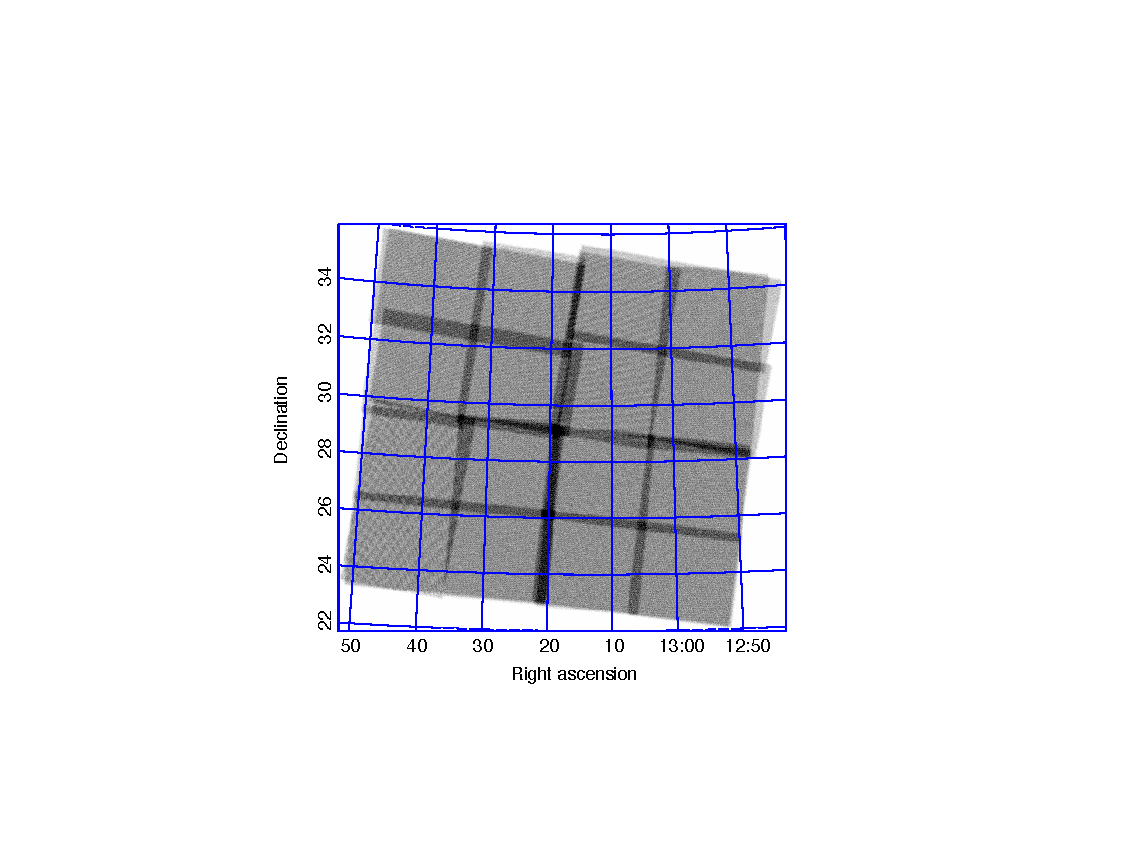
\includegraphics[scale=0.7]{ngpcoverage.pdf}
\caption{\protect\label{skymapn} The coverage map for 250\mic\ observations
of the NGP field.
The map shows the number of samples from the bolometer timelines contributing
to each map pixel, which ranges from 1 to 43, with the median value being 10.
The range of the grayscale is from 0 samples (white) to 27 samples
(black).}

\end{figure}

\begin{figure*} %2 
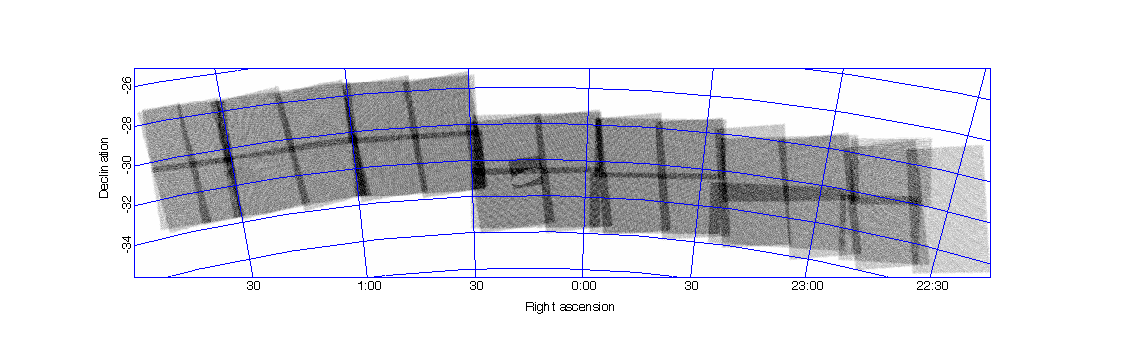
\includegraphics[scale=1.]{sgpcoverage.pdf}
\caption{ \protect\label{skymaps} 
The coverage map for 250\mic\ observations
of the SGP field.
The map shows the number of samples from the bolometer timelines contributing
to each map pixel, which ranges from 1 to 36, with the median value being 9.
The range of the grayscale is from 0 samples (white) to 21 samples
(black).}
\end{figure*}

\section{Source detection} 

\subsection{The maps and background subtraction} 

A detailed description of the processing necessary
to produce maps from the
Herschel raw data is presented in S17. The resulting maps maps have
pixel sizes 3, 4, 6, 8 and 12 arc seconds for 100, 160, 250, 350 and
500 $\mu$m respectively. The maps made with the PACS camera
(100 and 160\mic,\ Poglitsch et al. 2010) have units
of Jy per pixel. The maps made with the SPIRE camera
(250, 350 and 500\mic,\ Griffin et al. 2010) have units of Jy per beam.
The beam
areas at 250, 350 and 500\mic\ are 469, 831 and 1804 square arc seconds,
respectively.
The noise on the images is a combination of instrumental noise and the
confusion noise from sources that are too faint to be detected individually.
S17 describes a detailed analysis of the noise properties of the images.

Before attempting to detect sources in the maps, we first subtracted a
smoothly varying 'sky' level to remove the 
foreground emission from dust in our galaxy, so-called `cirrus emission',
and also the emission from
clustered extragalactic sources fainter
than
our detection limit. We
used the {\tt nebuliser} function, a programme produced
by the Cambridge Astronomy Survey Unit to estimate and
subtract the sky level on astronomical images (see
http://casu.ast.cam.ac.uk/surveys-projects/software-release/background-filtering). 

The
choice of the filter scale
used in {\tt nebuliser} is quite critical, since
it  must be small enough for {\tt nebuliser} to remove
small-scale patches of cirrus emission
but not so small that the flux from large galaxies is reduced.
In practice, 
for the SPIRE maps we found that a median filter scale of 30 pixels (3
arc minutes in the 250 \mic band) followed by a linear filter scale of
15 pixels was an acceptable combination. 

We tested 
whether this filtering scale reduced the flux density of extended extragalactic
sources
by creating
simulated maps, placing artificial extended sources on these maps, and then
measuring the flux densities of these sources
after the application of
{\tt nebuliser}. 
Since the nearby galaxies detected by {\it Herschel} are mostly
spiral galaxies,
we used exponential profiles for the artificial sources, convolving
these with the
SPIRE point-spread function.
The surface-brightness limit on photographic plates
is typically
$\rm \mu_B \simeq 25\ mag\ arcsec^{-2}$, giving rise
to the widely used D25 optical diameters for galaxies.
Since these diameters are roughly equivalent to a distance of five scale
lengths from the centre of a galaxy, we truncated the profiles
of our artificial submillimetre sources at five scale lengths,
which gave us diameters, roughly equivalent to D25 diameters in the optical
waveband, that ranged from
24 to 192 arcsec.
The simulations showed that significant flux is lost only for
sources that have diameters larger than $~3$ arc minutes, and even for
sources above this size,
the flux loss is $\lesssim 10\%$.

We note that the application of {\tt nebuliser} will change
the clustering statistics of extragalactic sources.
Apart from the foreground cirrus emission, {\tt nebuliser} removes
the background produced by the sources that are too faint to be detected
individually. This background varies because of the clustering of these
faint sources.
A source catalogue made
without any background subtraction will include more sources where the
this background is high as a result of clusters of these faint sources, and so
the clustering of the sources in this catalogue will be stronger than in
a catalogue produced from an image in which this background emission has been
removed. An investigation of the clustering in the H-ATLAS catalogues,
which includes an analysis of the effect of the subtraction of this
background, will be presented by Amvrosiadis et al. (in preparation).

For the PACS maps, the $1/f$-noise from the instrument is much larger than
for SPIRE, making the foreground cirrus emission and the background
emission from faint galaxies difficult to detect. Since we could not
clearly detect the foreground/background emission on smaller
scales, we used a {\tt nebuliser} scale of 5 arcminutes.

As the result
of the application of {\tt nebuliser}, the maps have a modal pixel value which is close to
zero. For the SPIRE bands, the instrumental noise is low enough that
the flux distribution of detected sources skews the pixel distribution to
positive values so the mean is slightly positive (1.0, 1.0 and 0.6
mJy/beam at 250, 350 and 500 \mic).
The PACS detector is less sensitive and less stable than SPIRE, and so the
instrumental noise dominates over the confusion noise and the pixel
distribution is close to Gaussian; the mean of the {\tt nebulised} PACS
maps are very close to zero (0.016 and 0.016
MJy/sr, respectively, for the 100 and 160\mic maps). 

\subsection{Source Detection} 


\begin{figure} %3 
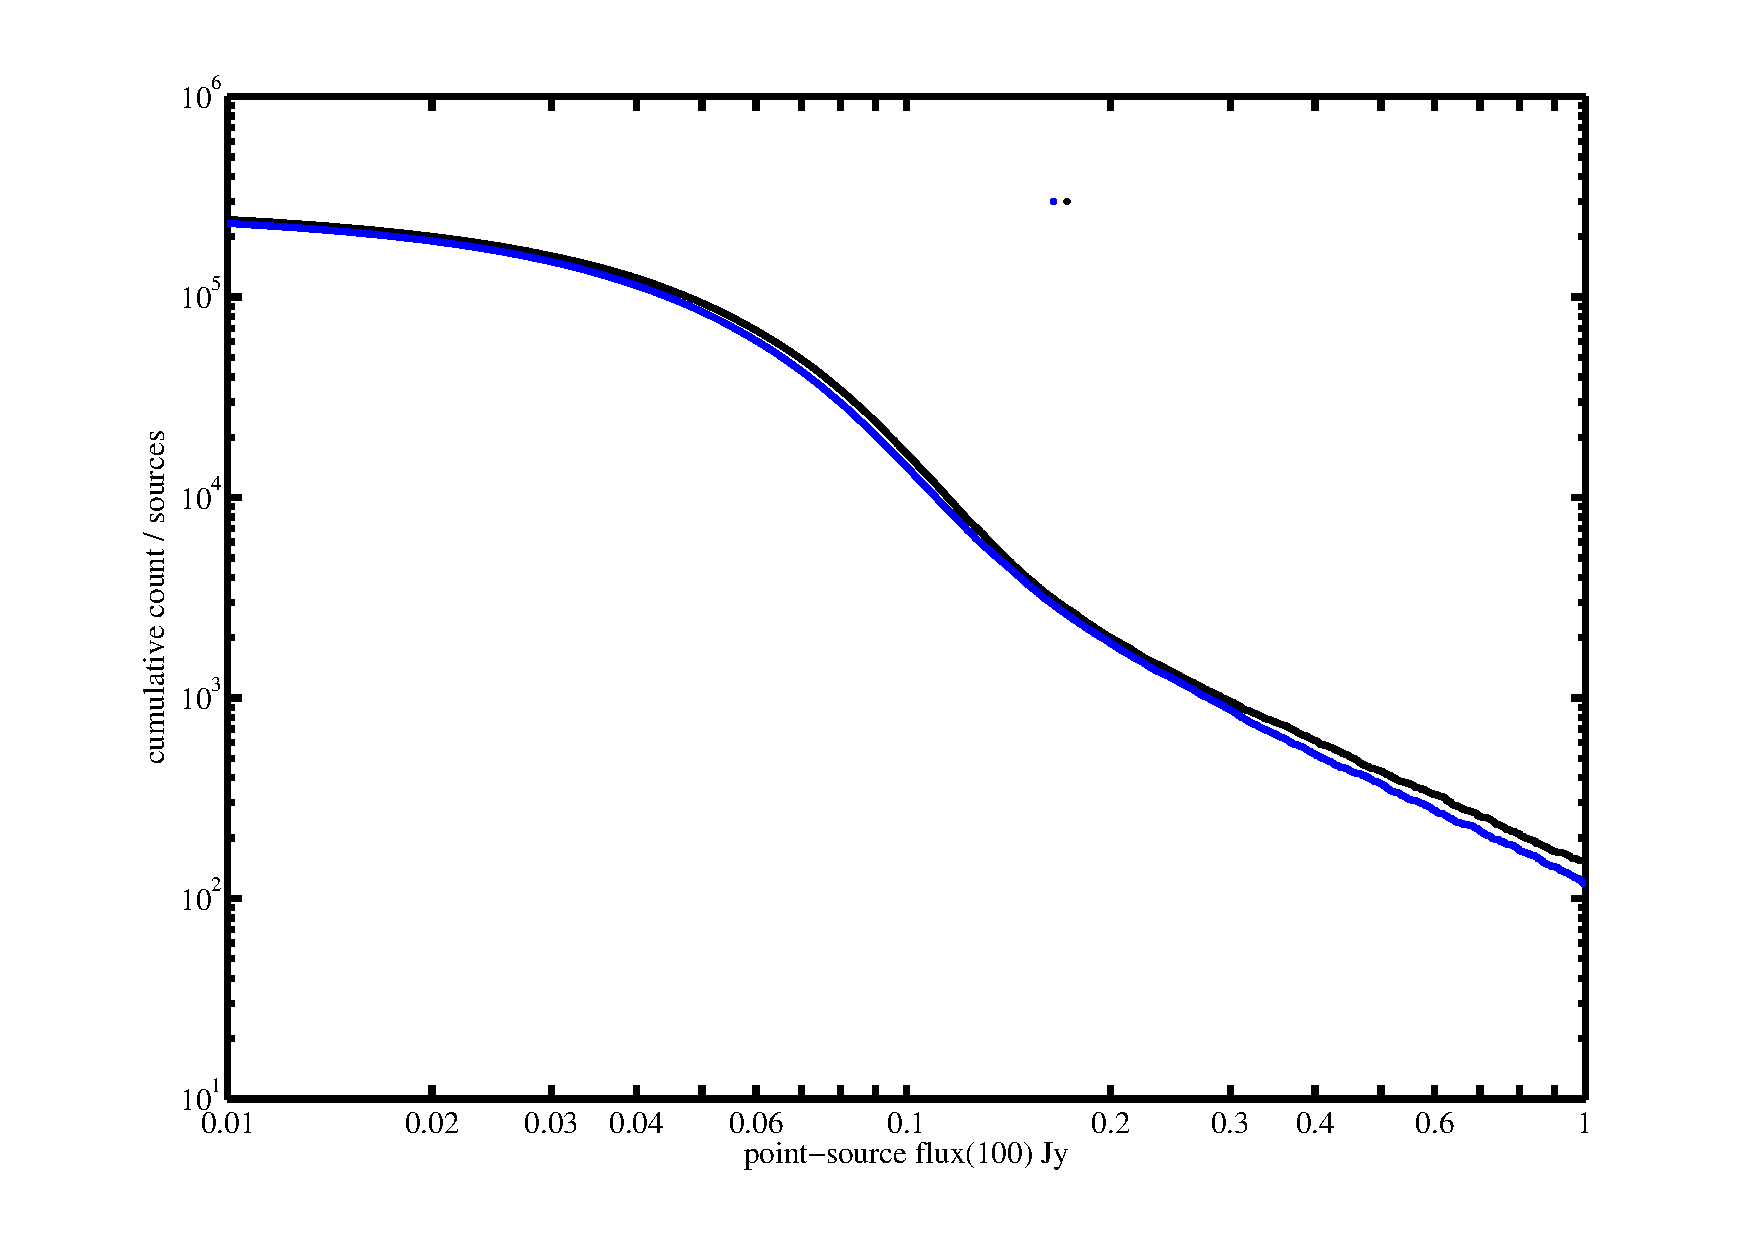
\includegraphics[width=0.42\textwidth,clip,trim={0 9mm 0mm 16mm}]{cum_counts_100.pdf}
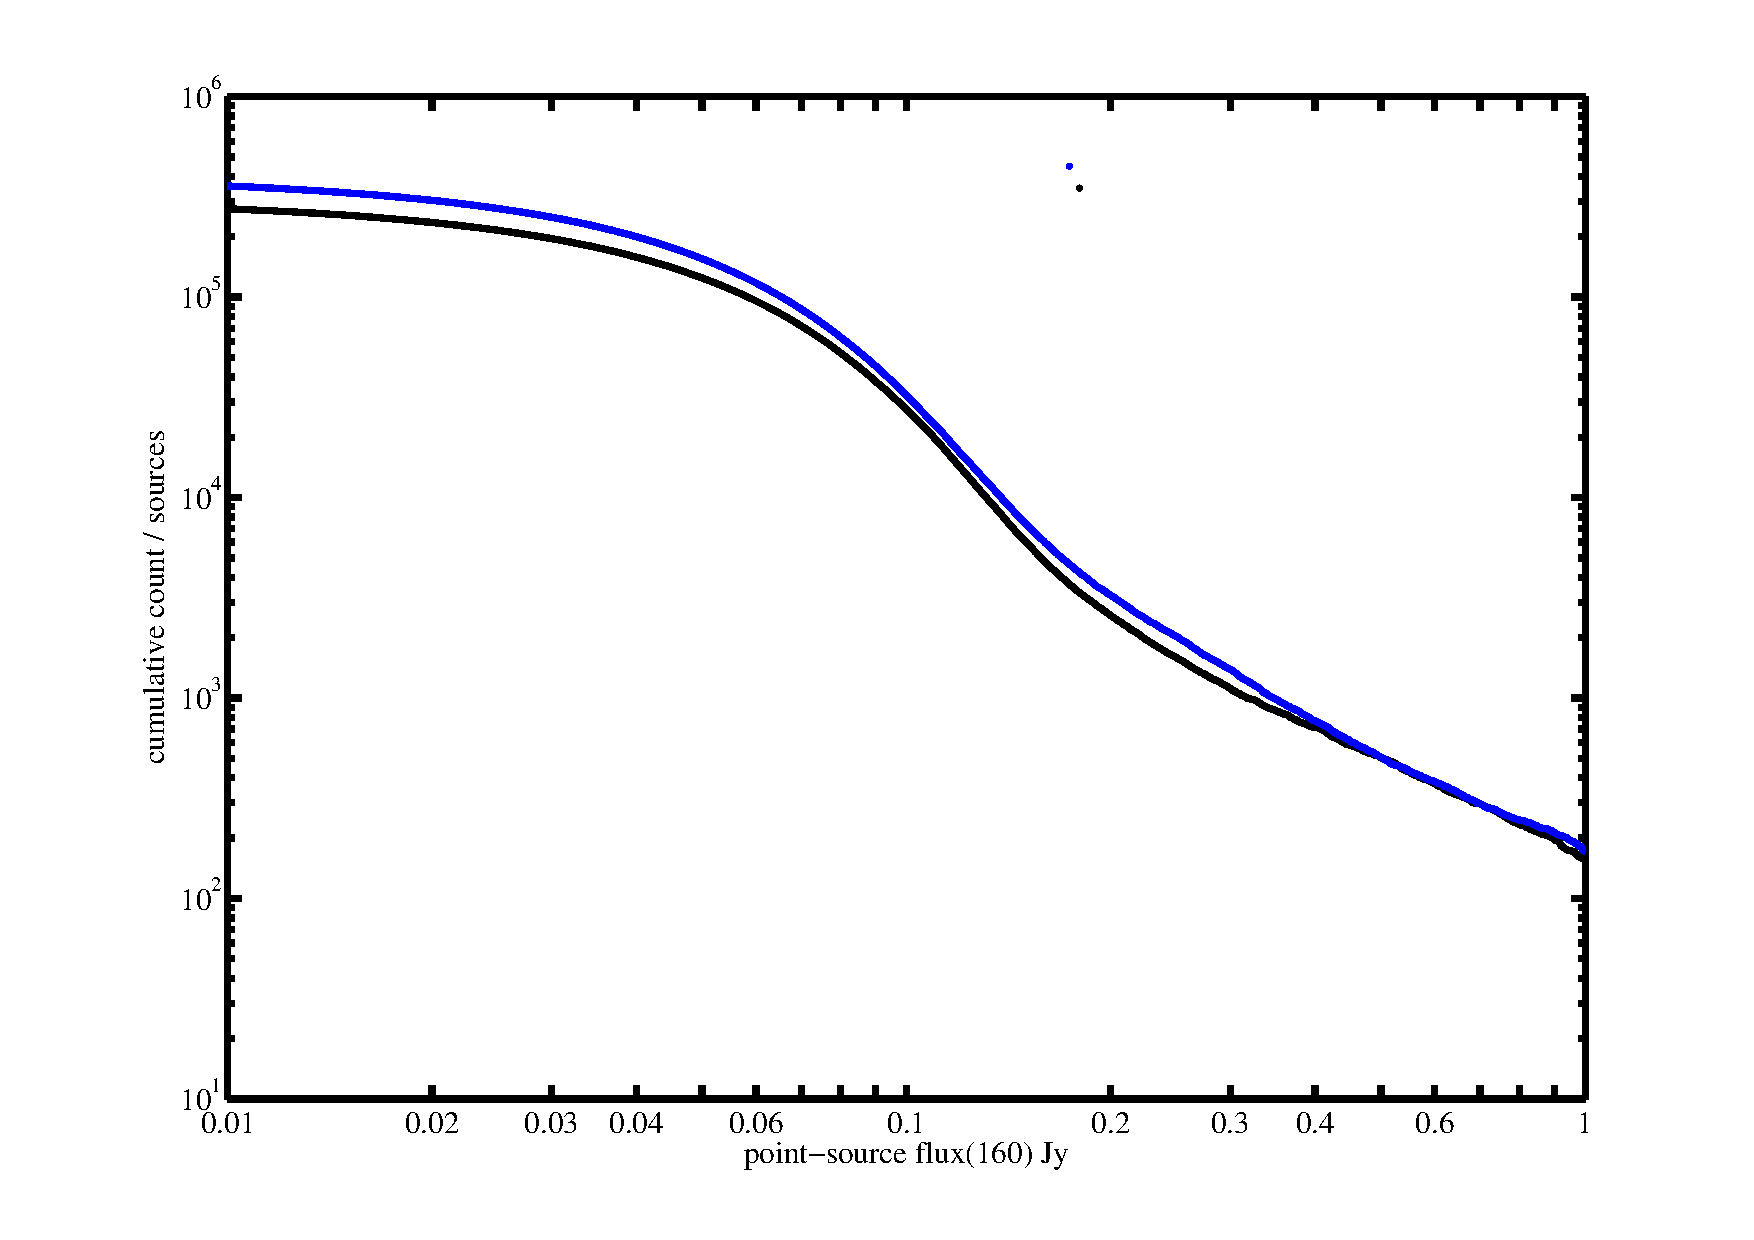
\includegraphics[width=0.42\textwidth,clip,trim={0 9mm 0mm 16mm}]{cum_counts_160.pdf}
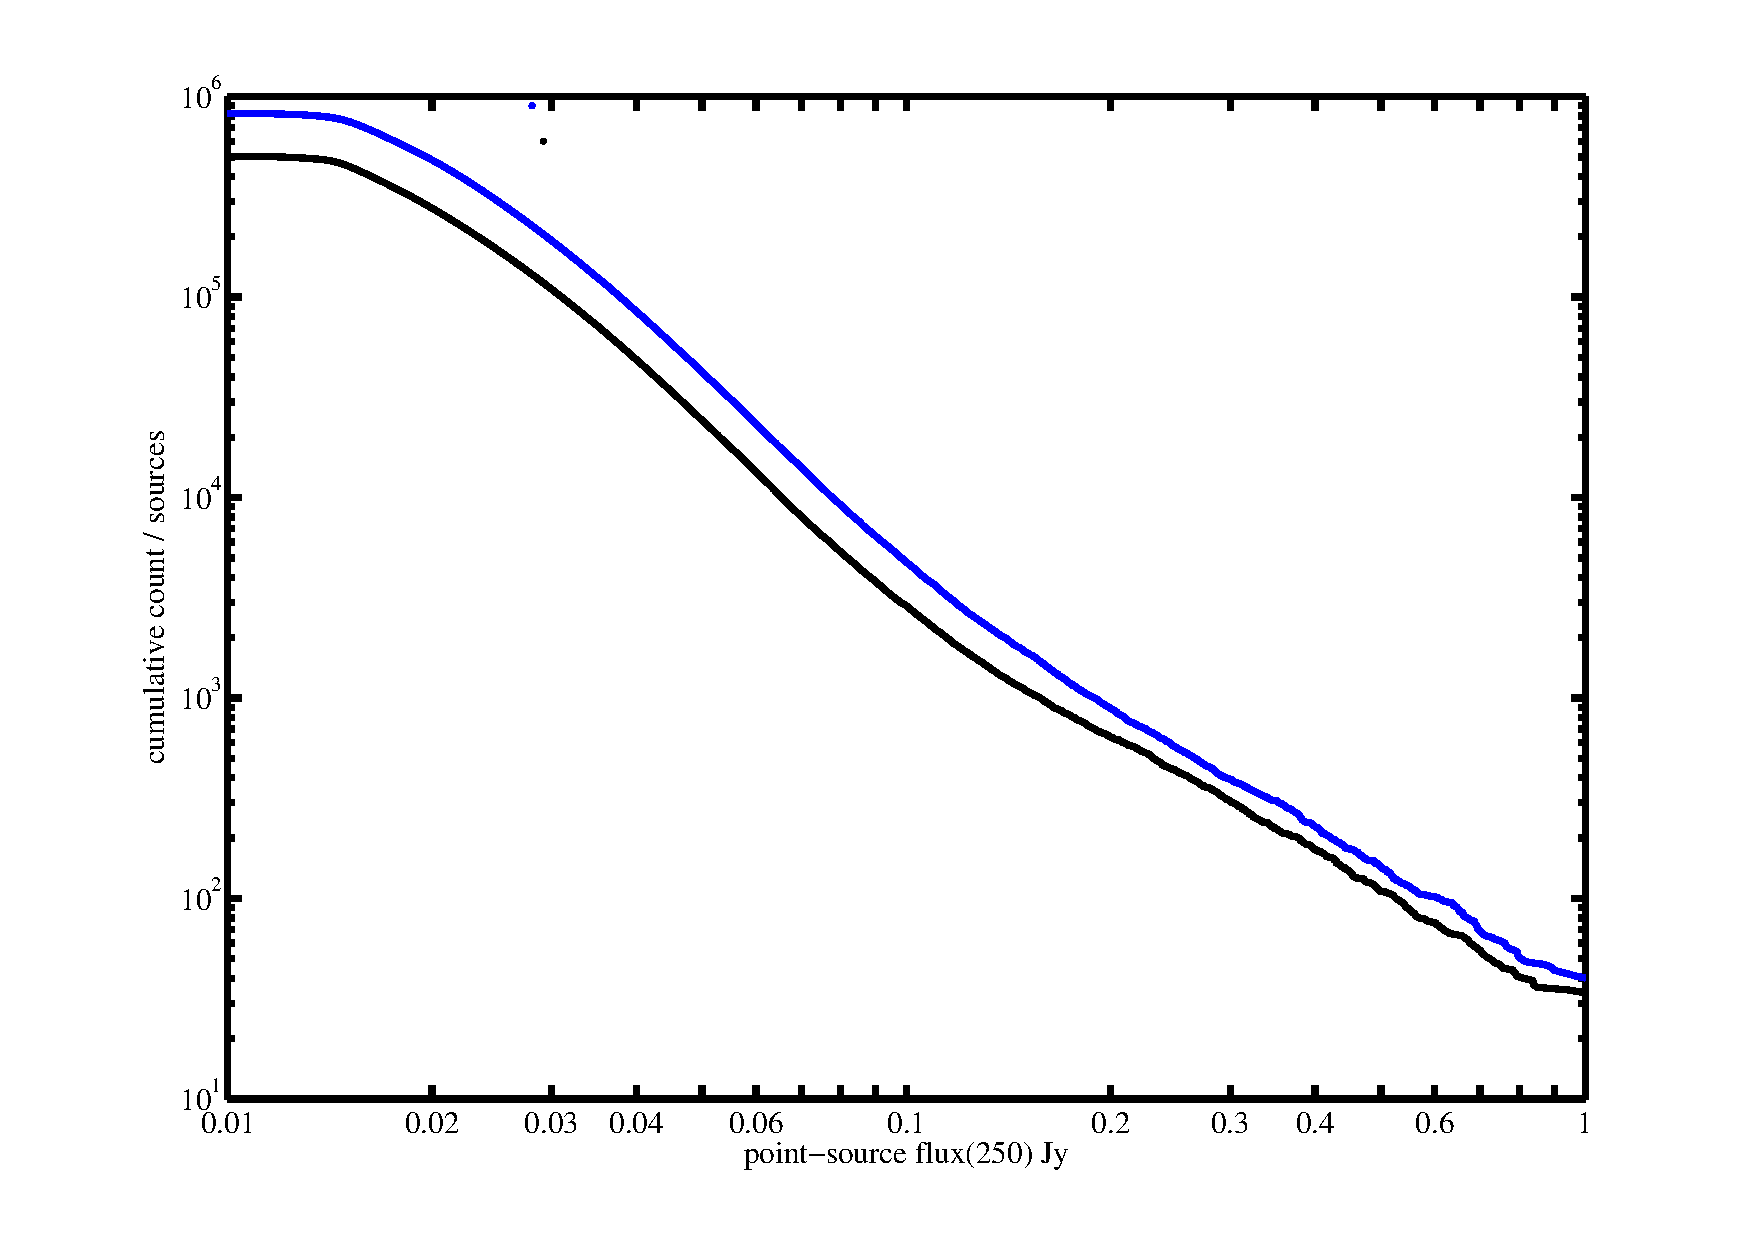
\includegraphics[width=0.42\textwidth,clip,trim={0 9mm 0mm 16mm}]{cum_counts_250.pdf}
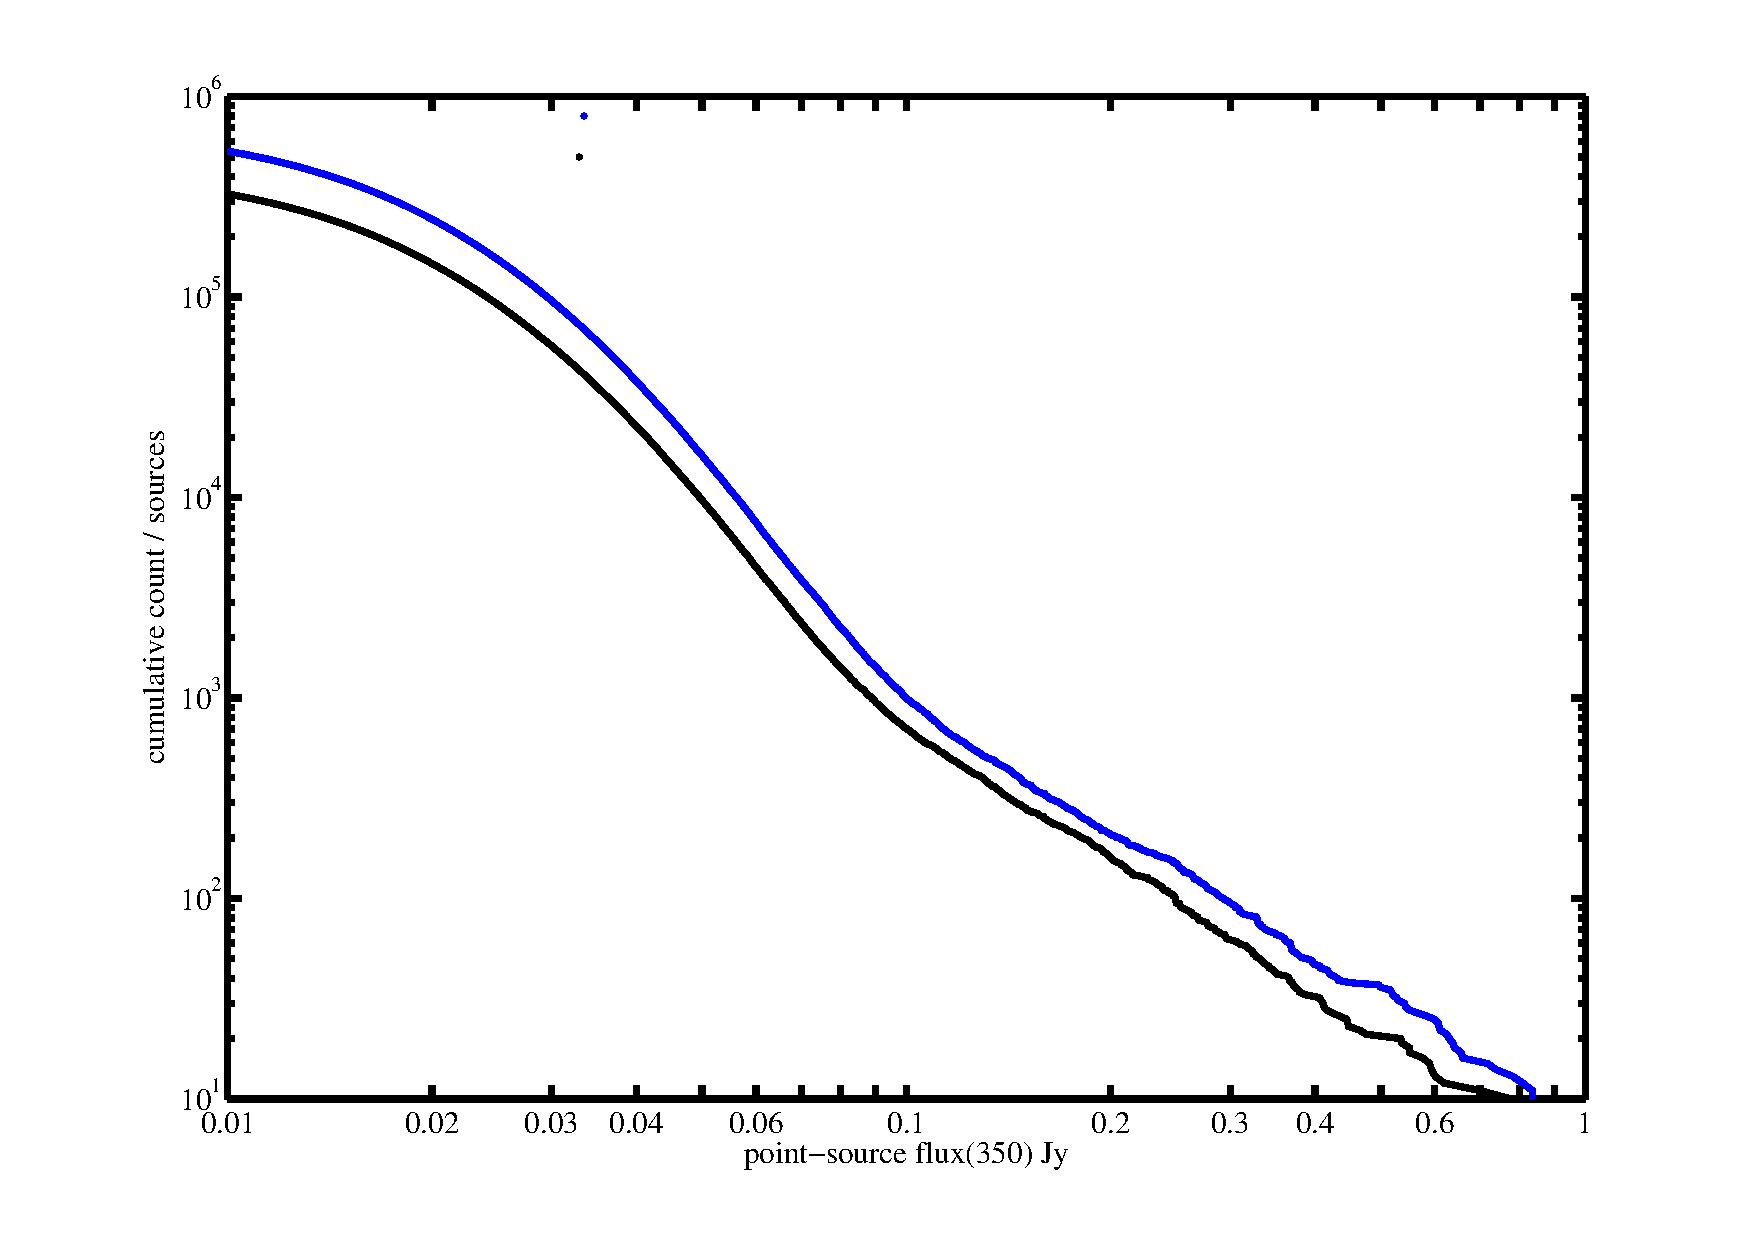
\includegraphics[width=0.42\textwidth,clip,trim={0 9mm 0mm 16mm}]{cum_counts_350.pdf}
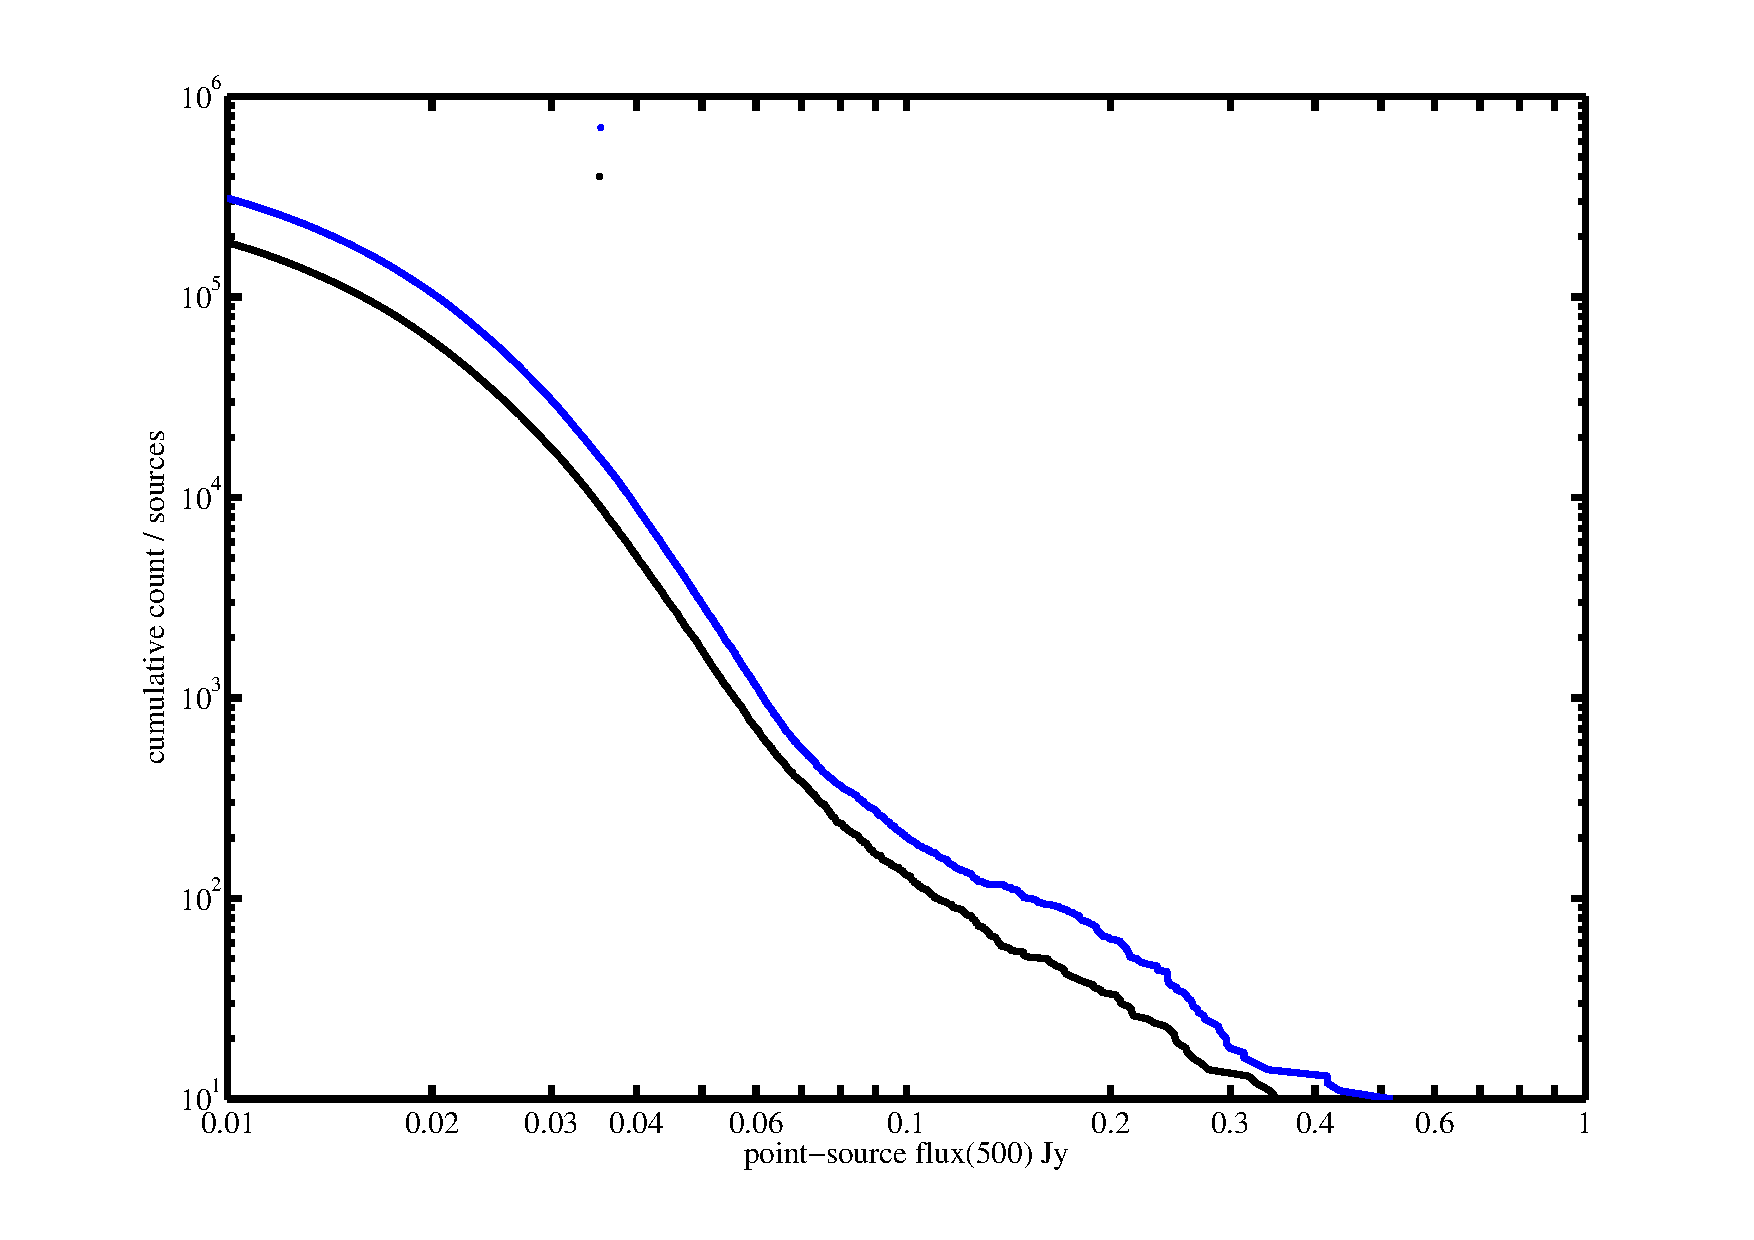
\includegraphics[width=0.42\textwidth,clip,trim={0 9mm 0mm 16mm}]{cum_counts_500.pdf}
\caption{\protect\label{fig_cum_flux} The cumulative number of sources as a
  function of flux at 100\mic, 160\mic, 250\mic, 350\mic and 500\mic. The NGP field is
shown in black; the SGP in blue. 
}
\end{figure}

In this section we describe the method used to find the
sources on the images. Additional details are given in V16.
Sources were detected using the MADX algorithm (Maddox et al in prep)
applied to the SPIRE maps.  MADX creates maps of the signal-to-noise
ratio and identifies sources by finding peaks in the signal to noise. The
detection and measurement of fluxes is optimised by using a matched
filter that is applied to both the signal map and the noise map. 

The SPIRE instrumental noise maps are created from the number of
detector passes and the estimated instrumental noise per pass,
$\sigma_{\mathrm inst} /\sqrt{N_ {\mathrm sample}}$, as described in S17 and V16.

%% the 2.5sig cut is instrumental only the 4 sigma includes both inst
%% and confusion
%% flux in other bands measured at optimal position, as defined from
%% the 250micron maps; there is a clean process for each band
%% individually
 
Since the noise consists of both instumental noise and
confusion noise from the background of undetected sources, we follow
the approach of Chapin et al (2011) to calculate the optimal matched
filter in each of the three SPIRE bands. Details of estimation and
form of the matched filter are discussed in V16.  The resulting
matched filters are slightly more compact than the corresponding PSFs,
and have slightly negative regions outside the FWHM.  

In the first step of the source detection, peak pixels which have
values $>2.5\sigma$ in the filtered 250\mic map are considered as
potential sources. 
We use the 250-$\mu$m map since most sources
have the highest signal-to-noise in this map.
The source 
position is determined by
fitting a Gaussian to the flux densities in the pixels surrouding
the pixel containing the peak emission.
As an initial estimate of the flux density of the
source in each SPIRE band, MADX takes the flux density in the
pixel closest to the 250-$\mu$m position.

The high source density on the SPIRE maps means that these flux estimates
often contain contributions from neighbouring sources.
To mitigate this effect, MADX uses the following procedure.
In each band, MADX sorts the sources in order of decreasing flux
density.
The
flux density of the brightest source is then
more precisely estimated from a bicubic interpolation
in the filtered map at the
250-$\mu$m position from the flux densities in the
$3 \times 3$ pixels around the position. 
Using this flux estimate, a point source profile is then subtracted
from the map at this position. The program then moves to the
next brightest source and follows the same set of steps.
One consequence of these steps
is that some sources will now have 250-$\mu$m flux densities
less than the
original $2.5\sigma$ cut. 
Since most sources are brighter at 250 $\mu$m than at the two
longer wavelengths, the estimates of the flux densities in the
350\mic and 500\mic bands are sometimes negative.

\section{Photometry}

\subsection{For point sources}

\subsubsection{SPIRE}

V16 carried out extensive simulations to determine the
errors on the flux density estimates for point sources.
They followed the simple procedure of injecting artificial
sources of known flux density on to the real maps and then
using MADX to estimate their flux densities
(Section 2.2).  
They found that at 250 $\mu$m, the detection
wavelength, the confusion noise varies as a function
of source flux and gave a simple formula to approximate this:
\smallskip
\begin{equation}
\sigma_{con250}^2 = \min(0.0049,f_{250}/5.6)^2 + 0.00253^2
\end{equation}
\smallskip
\noindent They found that
at 350\mic and 500\mic band the confusion noise 
is roughly constant, with $\sigma_{con350} = 0.00659$ and
$\sigma_{con500} = 0.00662$.

We calculated the errors in the flux density estimates for
each individual source, using these formulae to estimate
the confusion noise and the maps of the instrumental
noise (Section 2.2) to estimate the instrumental noise,
then adding the confusion and instrumental noise in
quadrature.

\subsubsection{PACS}

As in V16, we used aperture photometry to estimate the
flux densities in the two PACS bands. We did this for
two reasons. First, the
PACS PSF for our observing mode
(fast-parallel scan mode)
is not well determined near its peak (see V16 for an
extensive discussion). Second, if we estimated the 100 and
160-$\mu$m flux densities at the 250-$\mu$m position, as we
did for the 350 and 500-$\mu$m bands, we would be likely
to significantly underestimate the flux density because of
the higher resolution of the PACS maps.

V16 describe an extensive investigation of the optimum
aperture size, and we follow them in using an aperture
with a radius equal to the FWHM, which is
11.4 arc seconds for 100\mic and 13.7 arc seconds for
160\mic. Since the `sky' level has already been subtracted
with {\tt nebuliser}, we made no correction for any
residual sky level.
To reduce any pixelisation
effects, we divided each pixel into 16, assigning
one sixteenth of the flux density in each sub-pixel, and  
added up the flux density in each sub-pixel within the
aperture. 
Since only $\simeq$10\% of the
SPIRE sources were clearly detected on the PACS images,
we centered the aperture on the 250-$\mu$m position.

We corrected the aperture flux densities to
total flux densities using the 
table of the Encircled Energy Fraction (EEF)
described in V16 and available at {\tt
http://www.h-atlas.org/}.  
We made a further correction
to allow for the effect of the errors on the 250-$\mu$m positions,
since any error in the position will lead to the small PACS apertures
missing flux. V16 describe simulations of this effect, and we
follow them in compensating for this effect by multiplying the
flux densities by 1.1 and 1.05 at 100 and 160 $\mu$m, respectively.

We describe how we estimated the errors on these flux estimates in the
following section.

\subsection{Extended sources} 

The approach in the previous section
gives optimal flux density estimates for point sources, but will
seriously underestimate the flux density of extended sources. 
As in V16, we used the optical sizes of optical counterparts
to the {\it Herschel} sources to indicate which sources are
likely to require aperture photometry rather than the methods
described in the last section.
We followed different methods for the NGP and the SGP because
of the lack of a comprehensive identification analysis for the
SGP.

\subsubsection{The NGP}

In the NGP, F17 carried out a search for optical counterparts
to the {\it Herschel} sources on the r-band images
of the Sloan Digital Sky Survey (SDSS) which was almost exactly the
same as that carried out by Bourne et al. (2016) for the
H-ATLAS GAMA fields.
Our initial list of NGP sources that might require aperture
photometry were the sources with 
optical identifications
with reliability $R>0.8$ from F17.  

In our previous data release (V16) we calculated the sizes of
our apertures from 
the SDSS parameter
$\mathtt{isoA\_r}$, which was available in
SDSS DR7. However, this parameter was not available in SDSS
DR10, on which F17 based their analysis.
After an investigation of the various size measurements available
in DR10, we found that the parameter $\mathtt{petroR90\_r}$,
the 90\% Petrosian radius, met our needs since there
is a simple scaling betwen it and $\mathtt{isoA\_r}$,
with
$\mathtt{isoA\_r} \approx
1.156 \ \mathtt{petroR90\_r}$.

We considered that for H-ATLAS sources
with optical counterparts with $\mathtt{petroR90\_r}$ less than 8.6 arcsec (equivalent
to the value of $\mathtt{isoA\_r}$ of 10 arcsec used in V16)
the source
is still unlikely to be extended in the SPIRE bands, and for these H-ATLAS
sources we preferred the flux
densities in the SPIRE bands produced by MADX (Section 3.1.1).
However, if the H-ATLAS source had an optical counterpart
with $\mathtt{petroR90\_r}$ greater than 8.6 arcsec, and for
all PACS photometry, we measured aperture photometry.
We calculated the radius of the aperture using the 
same formula as V16 (with 
$\mathtt{isoA\_r}$ replaced by $\mathtt{petroR90\_r}$):
\smallskip
\begin{equation} 
r_\mathrm{ap} = \sqrt{ \mathtt{FWHM}^2 + {(1.156
    \ \mathtt{petroR90\_r})}^2}\ , 
\end{equation}
\smallskip
where $\mathtt{FWHM}$ is the Full-Width Half-Maximum of the point-spread
function for the passband being measured. As discussed above
(Section 3.1.2), we also use aperture photometry
in the PACS bands for sources without reliable optical counterparts,
using an aperture with a radius equal to the FWHM.

After calculating the aperture using
equation 2, we visually compared it with
the 250-$\mu$m emission from the
source, since in some case the aperture is not well-matched
to the 250-$\mu$m emission, either being too small, too large,
with the wrong shape or including the flux from a neighbouring
galaxy (see V16 for examples). 
In these cases, we chose
a more appropriate aperture for the galaxy. 
We also visually inspected the 3000 sources with the brightest
250-$\mu$m flux densities from MADX in order to check whether
there were any obvious additional extended sources. 
For these sources too, we chose appropriate apertures
to include all of the emission.
In total, for the NGP there are 74 of these `customised apertures'.
The details
of these customised apertures are given as part of the
data release.

We calculated errors in the aperture flux densities from the
results of the Monte-Carlo simulation of S17. S17
placed apertures randomly on the SGP and NGP
maps in areas which are made from two individual observations
($N_{scan}=2$), varying the aperture radii from approximately
the beam size up to 100$''$ in 2$''$ intervals and using 3000
random positions for each aperture radius.
They found that the error, $\sigma_{ap}$, depends on the radius
the aperture as a double power-law:

\begin{equation}
  \sigma_{\mathrm{ap}}(\mathrm{mJy}) =
  \begin{cases}
      Ar^\alpha &   \mathrm{if\ } r\le 50'' \\
      B(r-50)^\beta + A 50^\alpha & \mathrm{for\ } r>50''
    \end{cases}
\end{equation}

The constants $A$, $B$, $\alpha$, and $\beta$  are given in Table~3 of S17.
We used this equation for the sources on parts of the images made from two
observations. In parts of the images made from more than two observations
the instrumental noise is less; for sources in these more sensitive parts of
the images we used the extension of equation 3 derived by S17: equation
4 in S17 for SPIRE and equation 6 in S17 for PACS.

Finally, we only used the aperture flux density if
it is significantly larger than the point-source estimate, if
\begin{equation}
F_\mathrm{ap}- F_\mathrm{ps}>\sqrt{\sigma_\mathrm{ap}^2-\sigma_\mathrm{ps}^2}
\ .
\end{equation}

In summary, of the 118,986 sources in the NGP, we measured aperture
flux densities at 250 $\mu$m for 889 sources. 

\subsubsection{The SGP}

For the SGP area no SDSS data exists
and we have not carried out the comprehensive identification analysis
that we have carried out for the other four fields. Instead, we have
carried out a rudimentary identification analysis using the
2MASS survey. We first found a 2MASS galaxy parameter that provides
a useful estimate of the size of the galaxy. We found that
the 2MASS parameter $\mathtt{sup\_r\_3sig}$
(super-coadd 3-sigma isophotal semi-major
axis) has a simple scaling with the
$\mathtt {isoA\_r}$:
$\mathtt{isoA\_r} \approx 1.96 \ \mathtt{sup\_r\_3sig}$.
We found all 2MASS galaxies in the SGP region with $\mathtt{sup\_r\_3sig}>5.1$ arcsec,
equivalent to $\mathtt{isoA\_r}=10\ arcsec$. There are 6249 of these
galaxies. We then found all H-ATLAS sources in the SGP within 5 arcsec
of a 2MASS galaxy. There are 3444 of these sources, and a simple
probability analysis shows that only 23 (0.7\%) of these matches
should not be physical associations of the
H-ATLAS source and the 2MASS galaxy.

For these sources, we calculated the radius of the aperture
to use for photometry using the relationship:
\smallskip
\begin{equation} 
r_\mathrm{ap} = \sqrt{ \mathtt{FWHM}^2 + {(1.96
    \ \mathtt{sup\_r\_3sig})}^2}\ .
\end{equation}
\smallskip
\noindent This is the same as equation 2, except for the change
in the parameter used to estimate the size of the galaxy.

As for the NGP, we then visually compared the apertures
with the 250-$\mu$m emission from the source, modifying the aperture
when necessary (see above). 
We also visually inspected the 5000 sources with the brightest
250-$\mu$m flux densities from MADX in order to check whether
there were any obvious additional extended sources. 
For these sources too, we chose appropriate apertures
to include all of the emission.
In total, for the SGP there are XXX customised apertures, for which the
details are given as part
of the
data release.

In the case of the SGP, 
we centered the apertures on the
250-$\mu$m positions rather than on the optical positions.
Since the `sky' level on both the PACS and SPIRE images
 has already been subtracted
with {\tt nebuliser}, we made no correction for any
residual sky level.
To reduce any pixelisation
effects, we divided each pixel into 16, assigning
one sixteenth of the flux density in each sub-pixel, and
added up the flux density in each sub-pixel within the
aperture.
We corrected the PACS flux densities to
total flux densities using the
table EEF
described in V16 and available at {\tt
http://www.h-atlas.org/}.
We corrected all the 
SPIRE aperture flux densities for the fraction of the PSF outside the aperture
using a table of 
corrections determined from the best estimate of the SPIRE PSF (Griffin et al. 2013),
which is provided as part of the data release (see V16 for more details).

We followed the same procedure for estimating the errors in the
flux densities and for deciding whether to use the aperture flux
density rather than the flux density from MADX as for the NGP.
In summary, of the XXX sources in the SGP, we measured aperture
flux densities at 250 $\mu$m for XXX sources. 

\begin{figure}
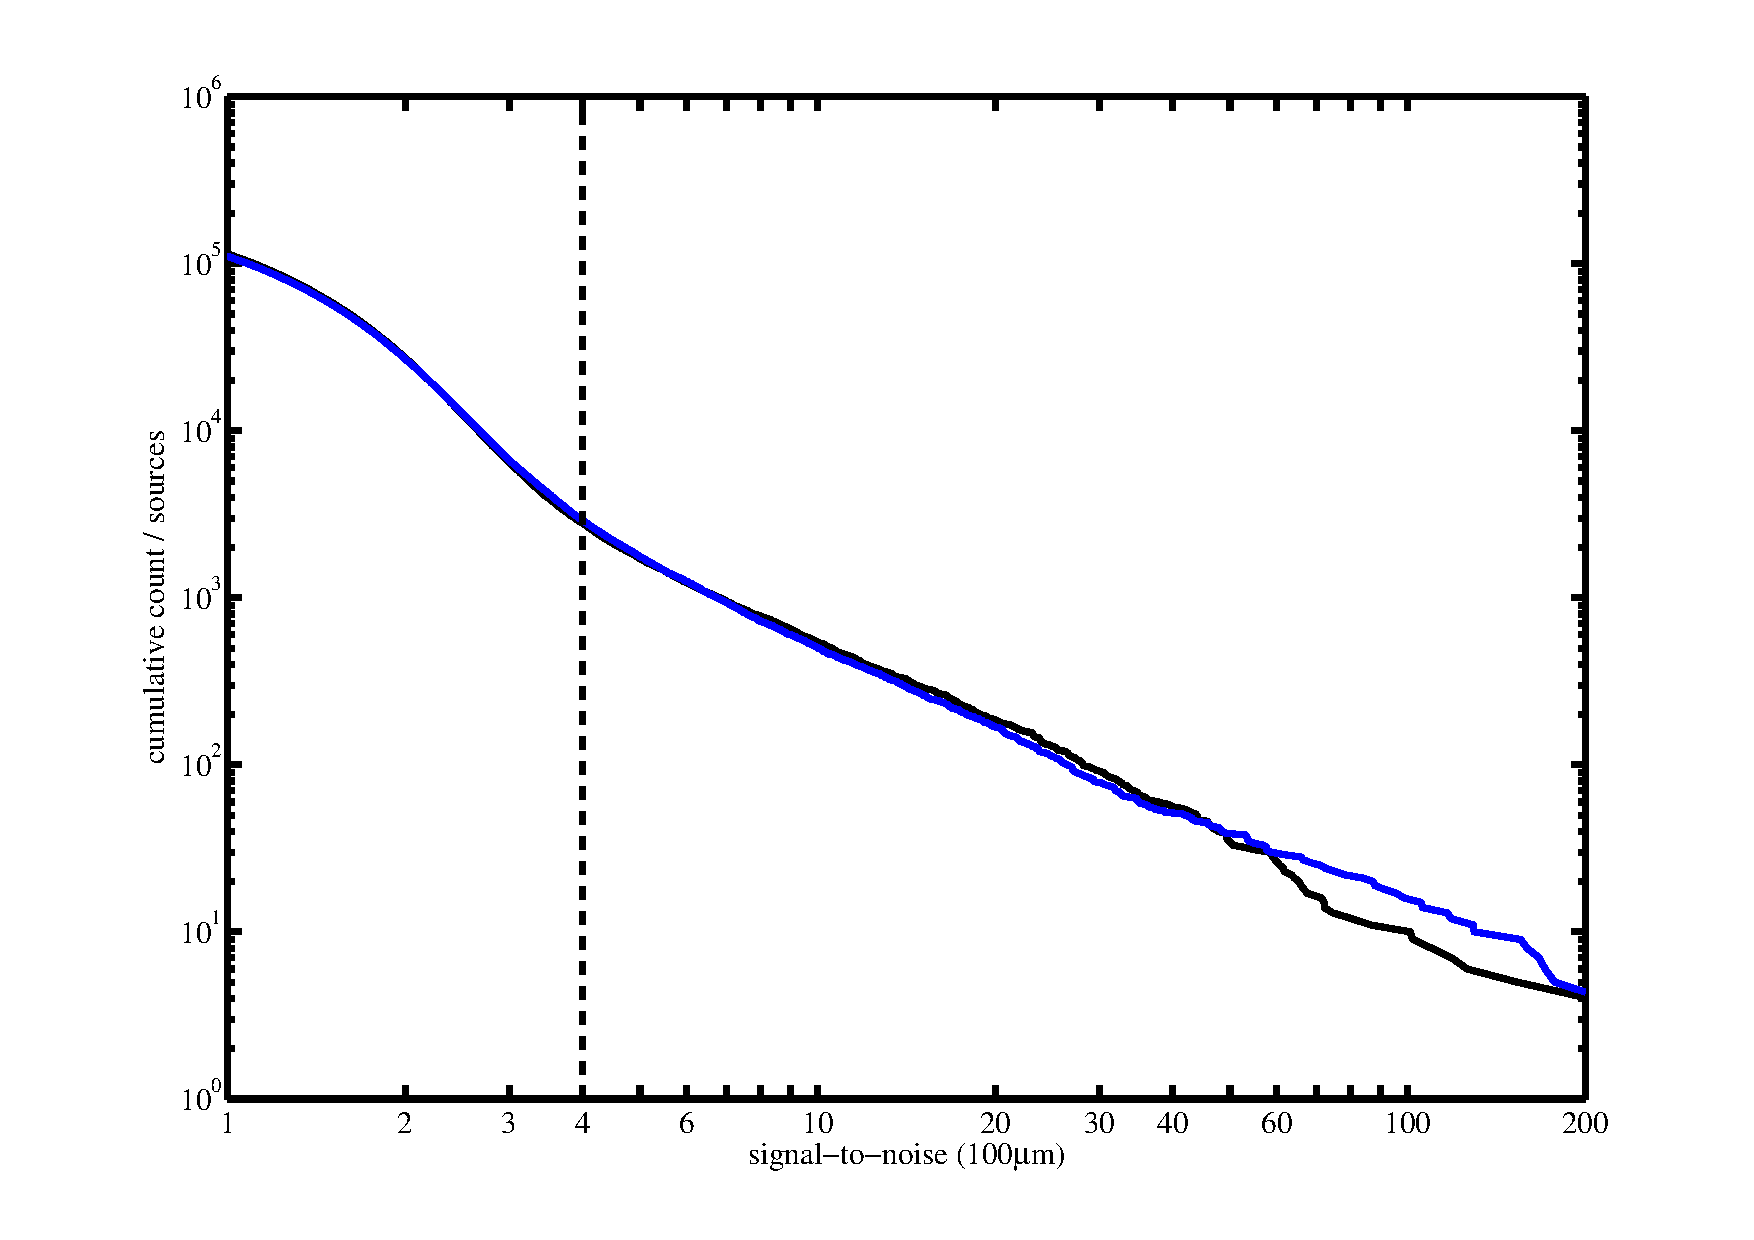
\includegraphics[width=0.42\textwidth,clip,trim={0 9mm 0mm 16mm}]{cum_sn_100.pdf}
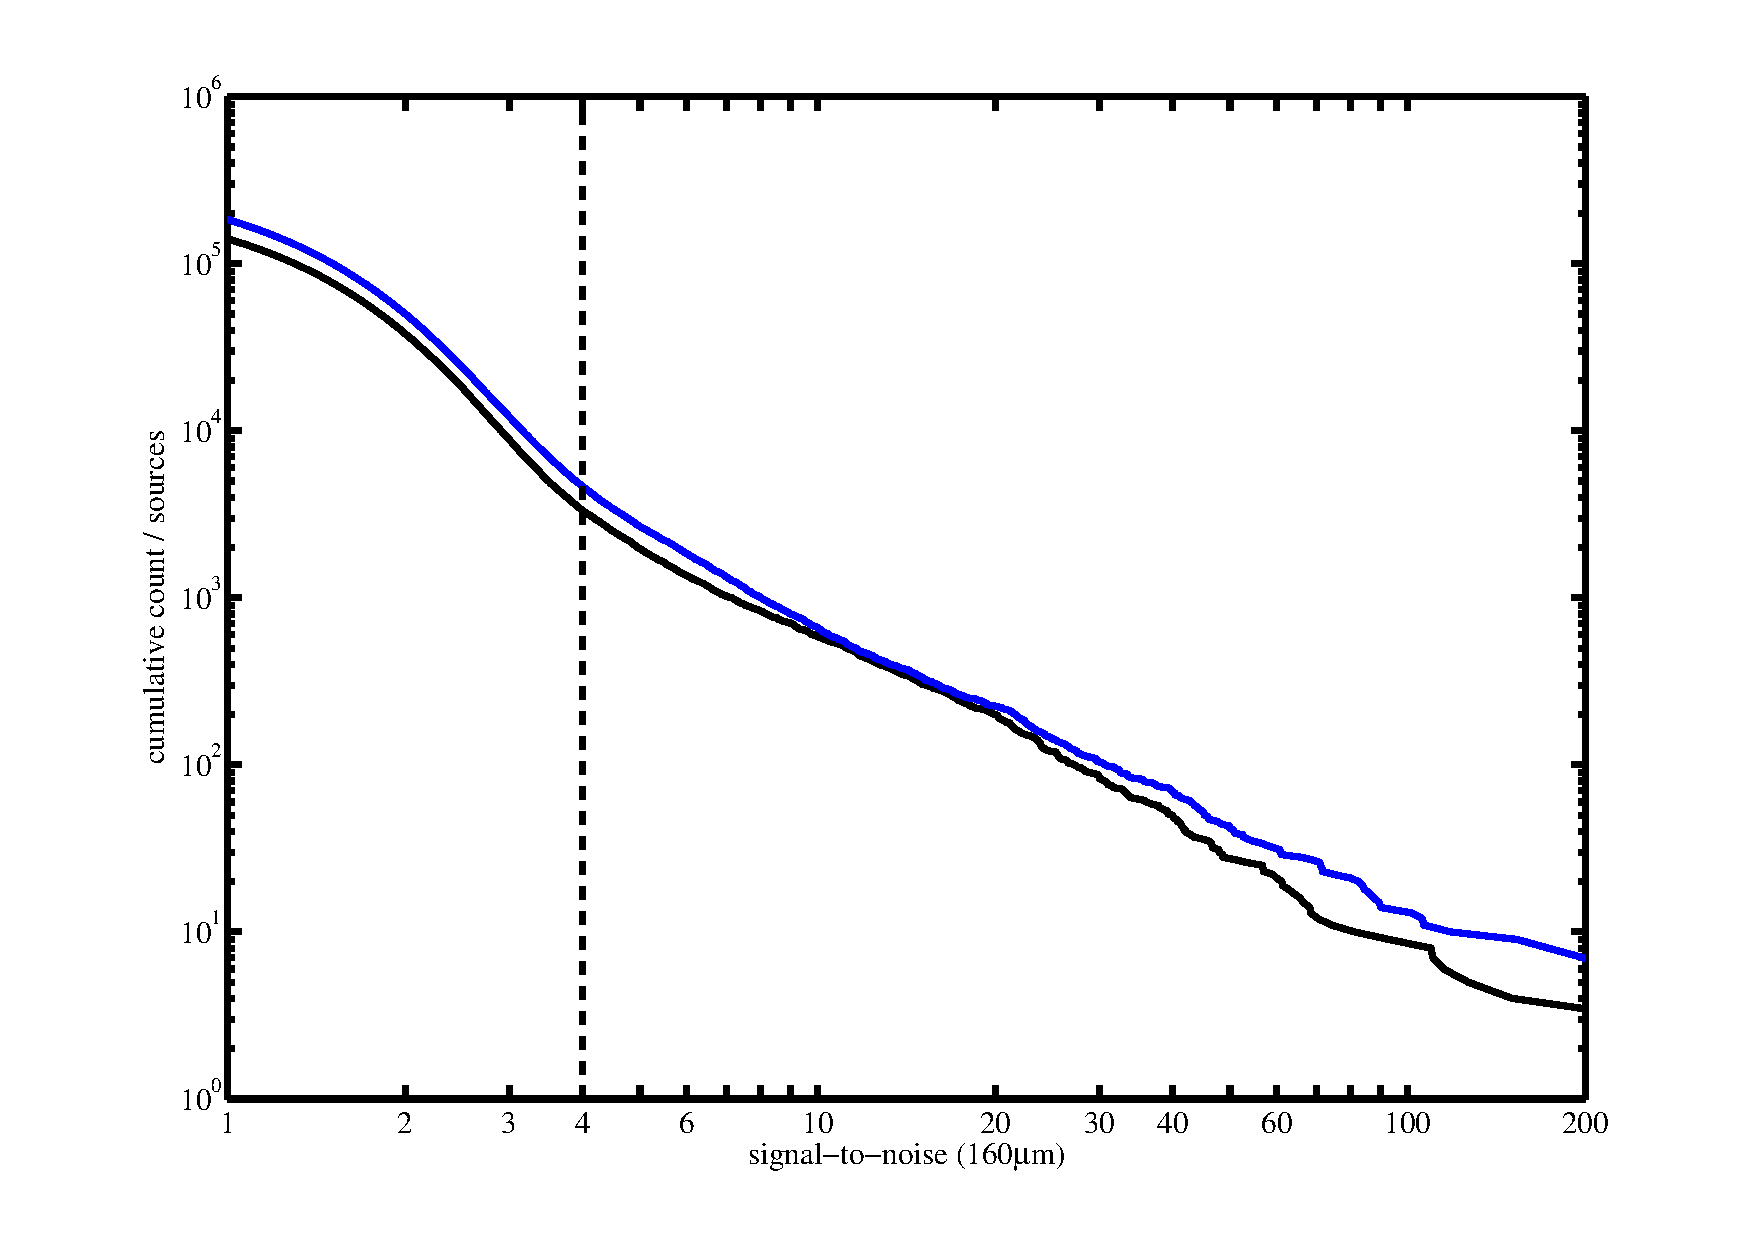
\includegraphics[width=0.42\textwidth,clip,trim={0 9mm 0mm 16mm}]{cum_sn_160.pdf}
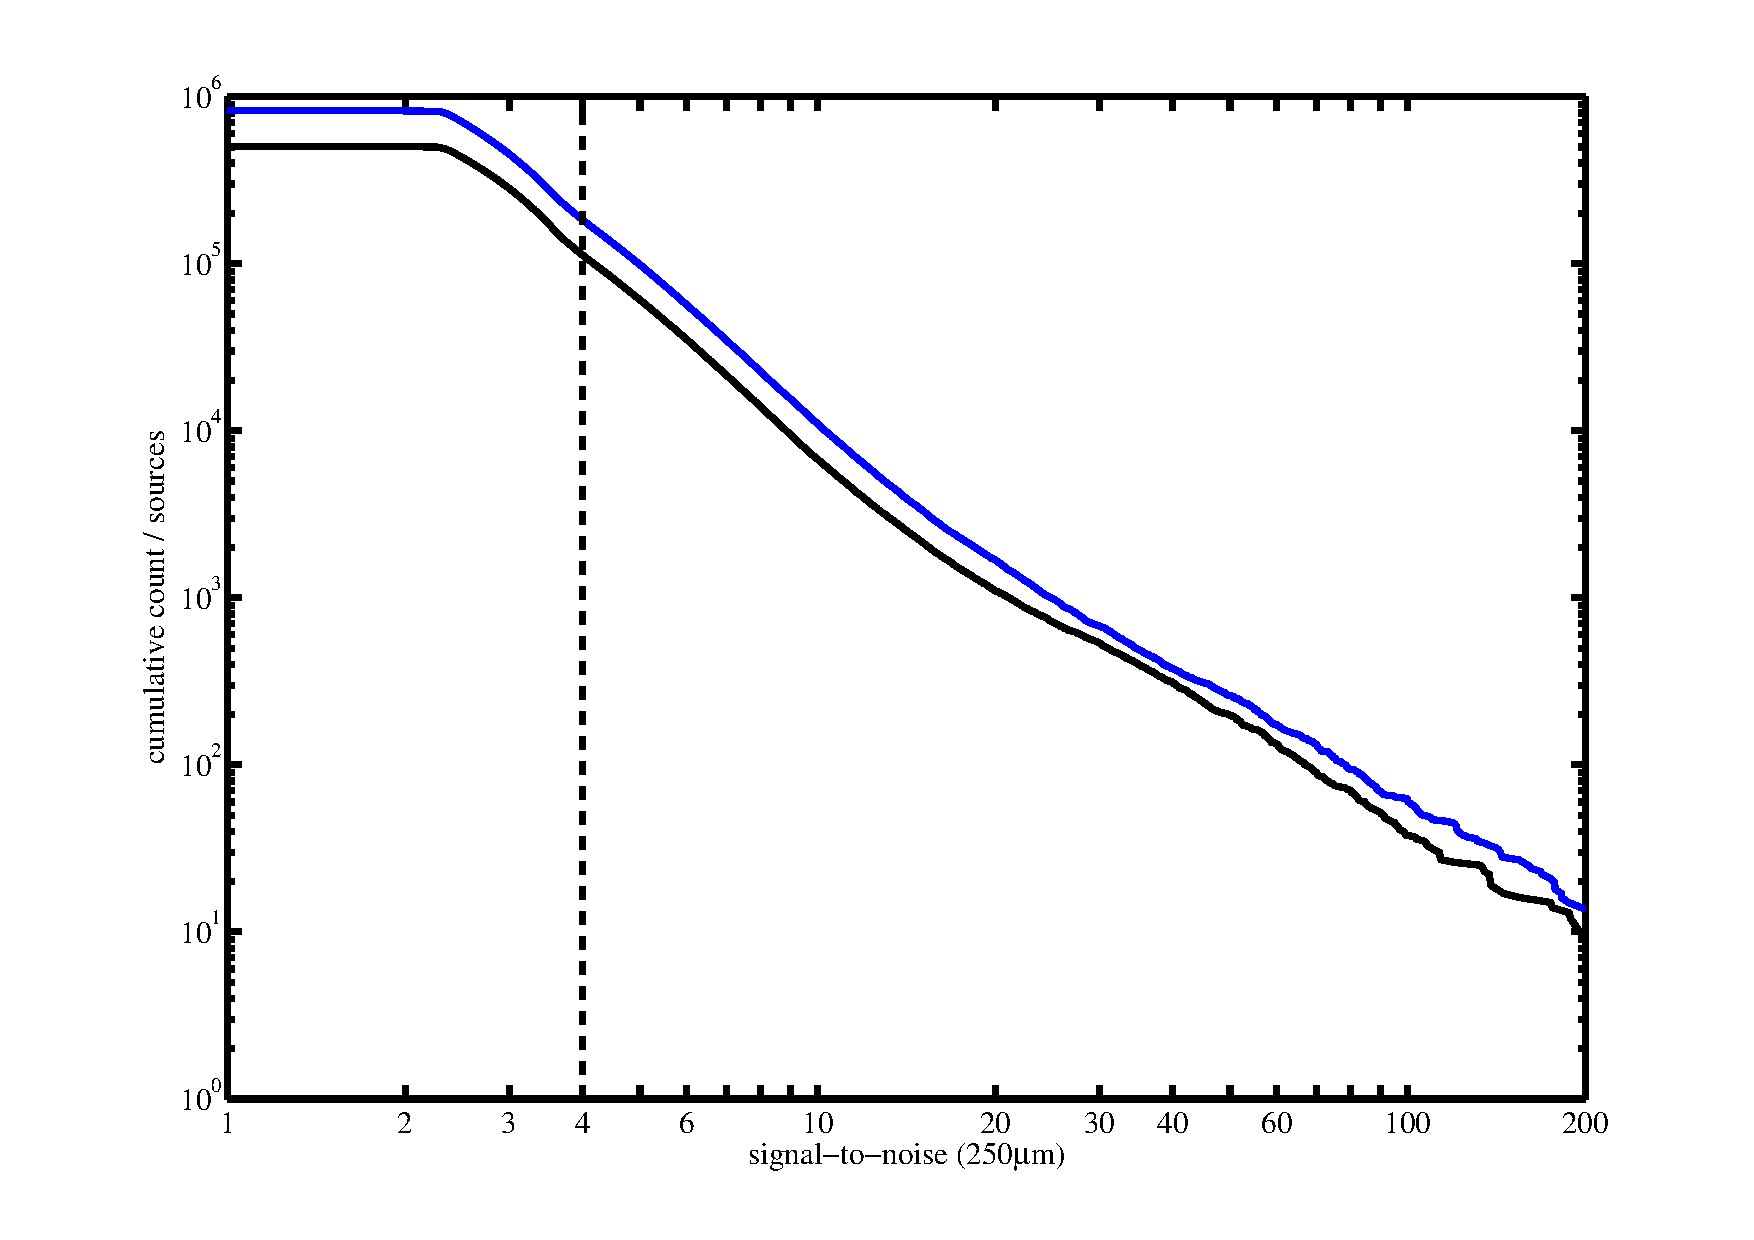
\includegraphics[width=0.42\textwidth,clip,trim={0 9mm 0mm 16mm}]{cum_sn_250.pdf}
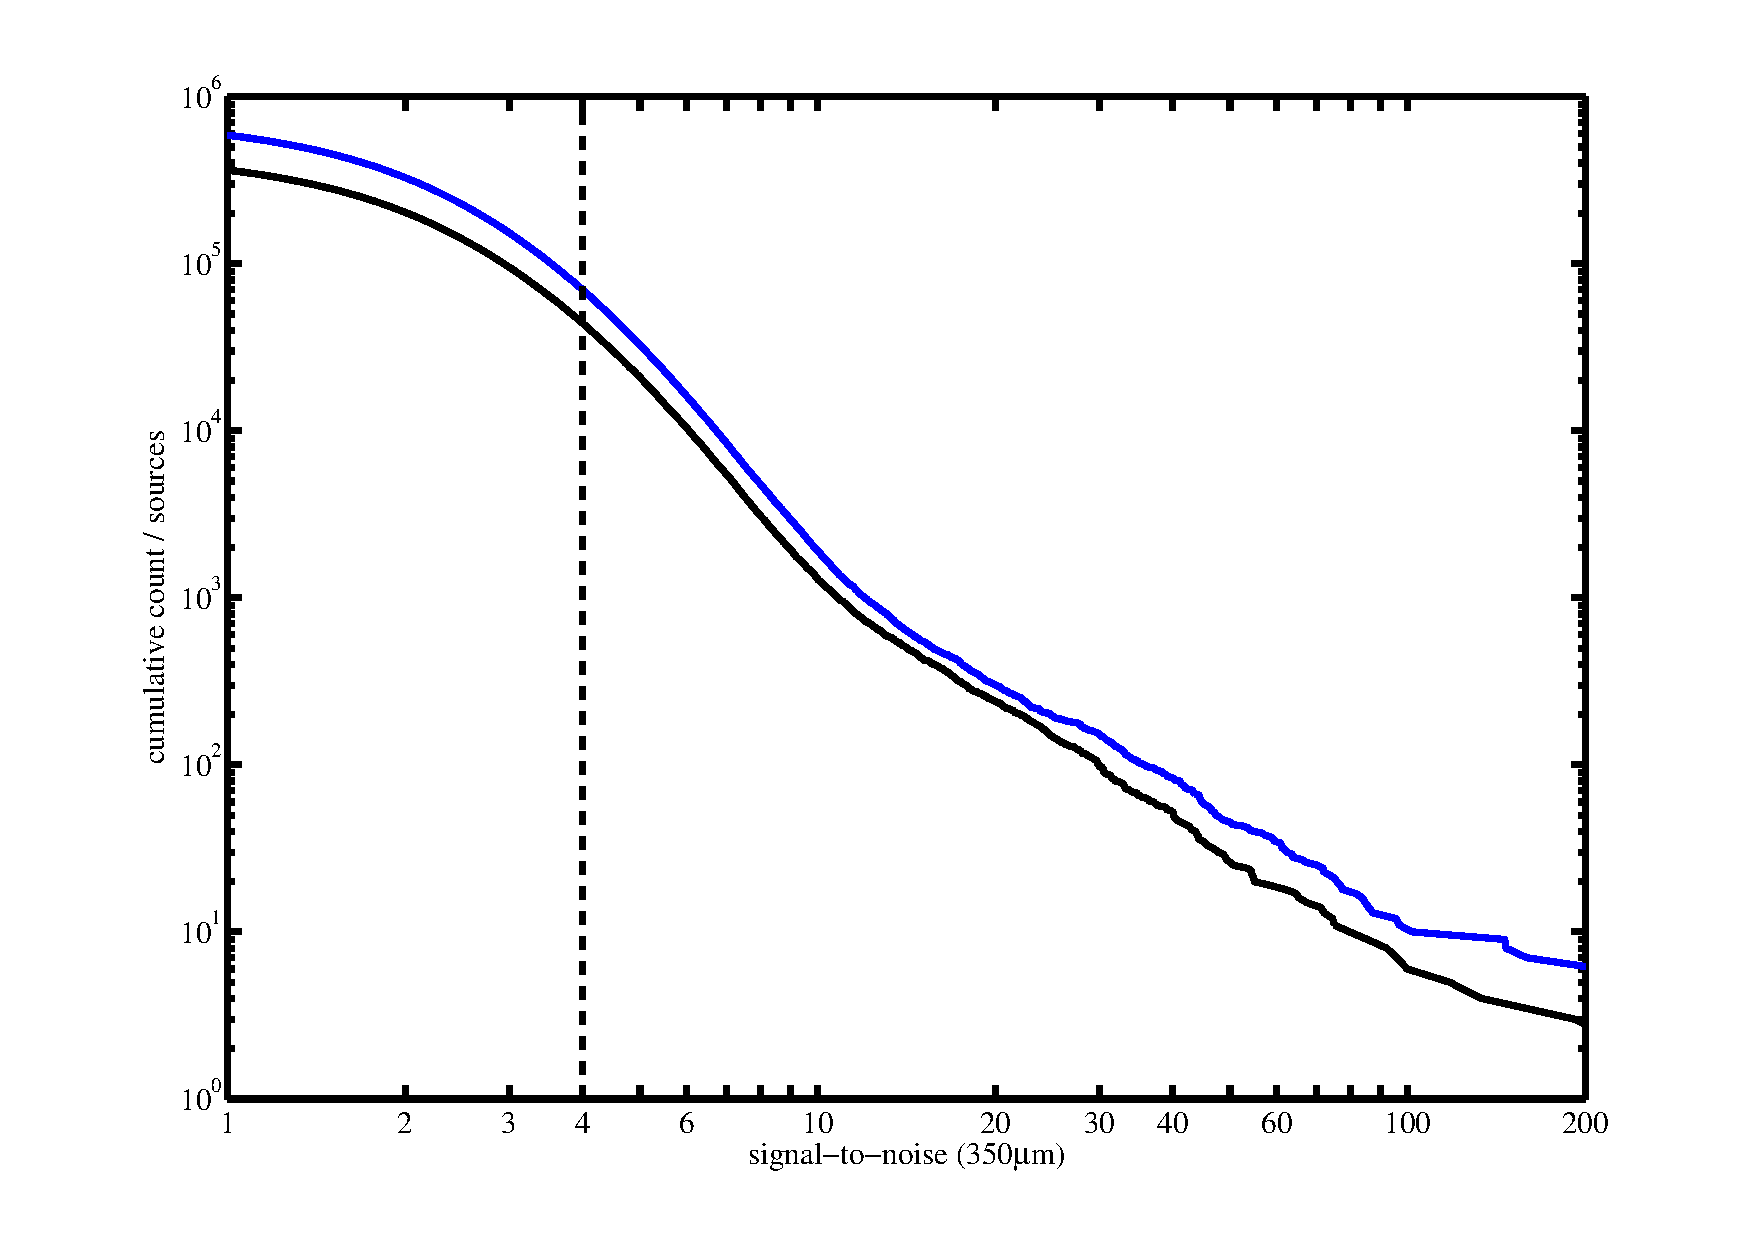
\includegraphics[width=0.42\textwidth,clip,trim={0 9mm 0mm 16mm}]{cum_sn_350.pdf}
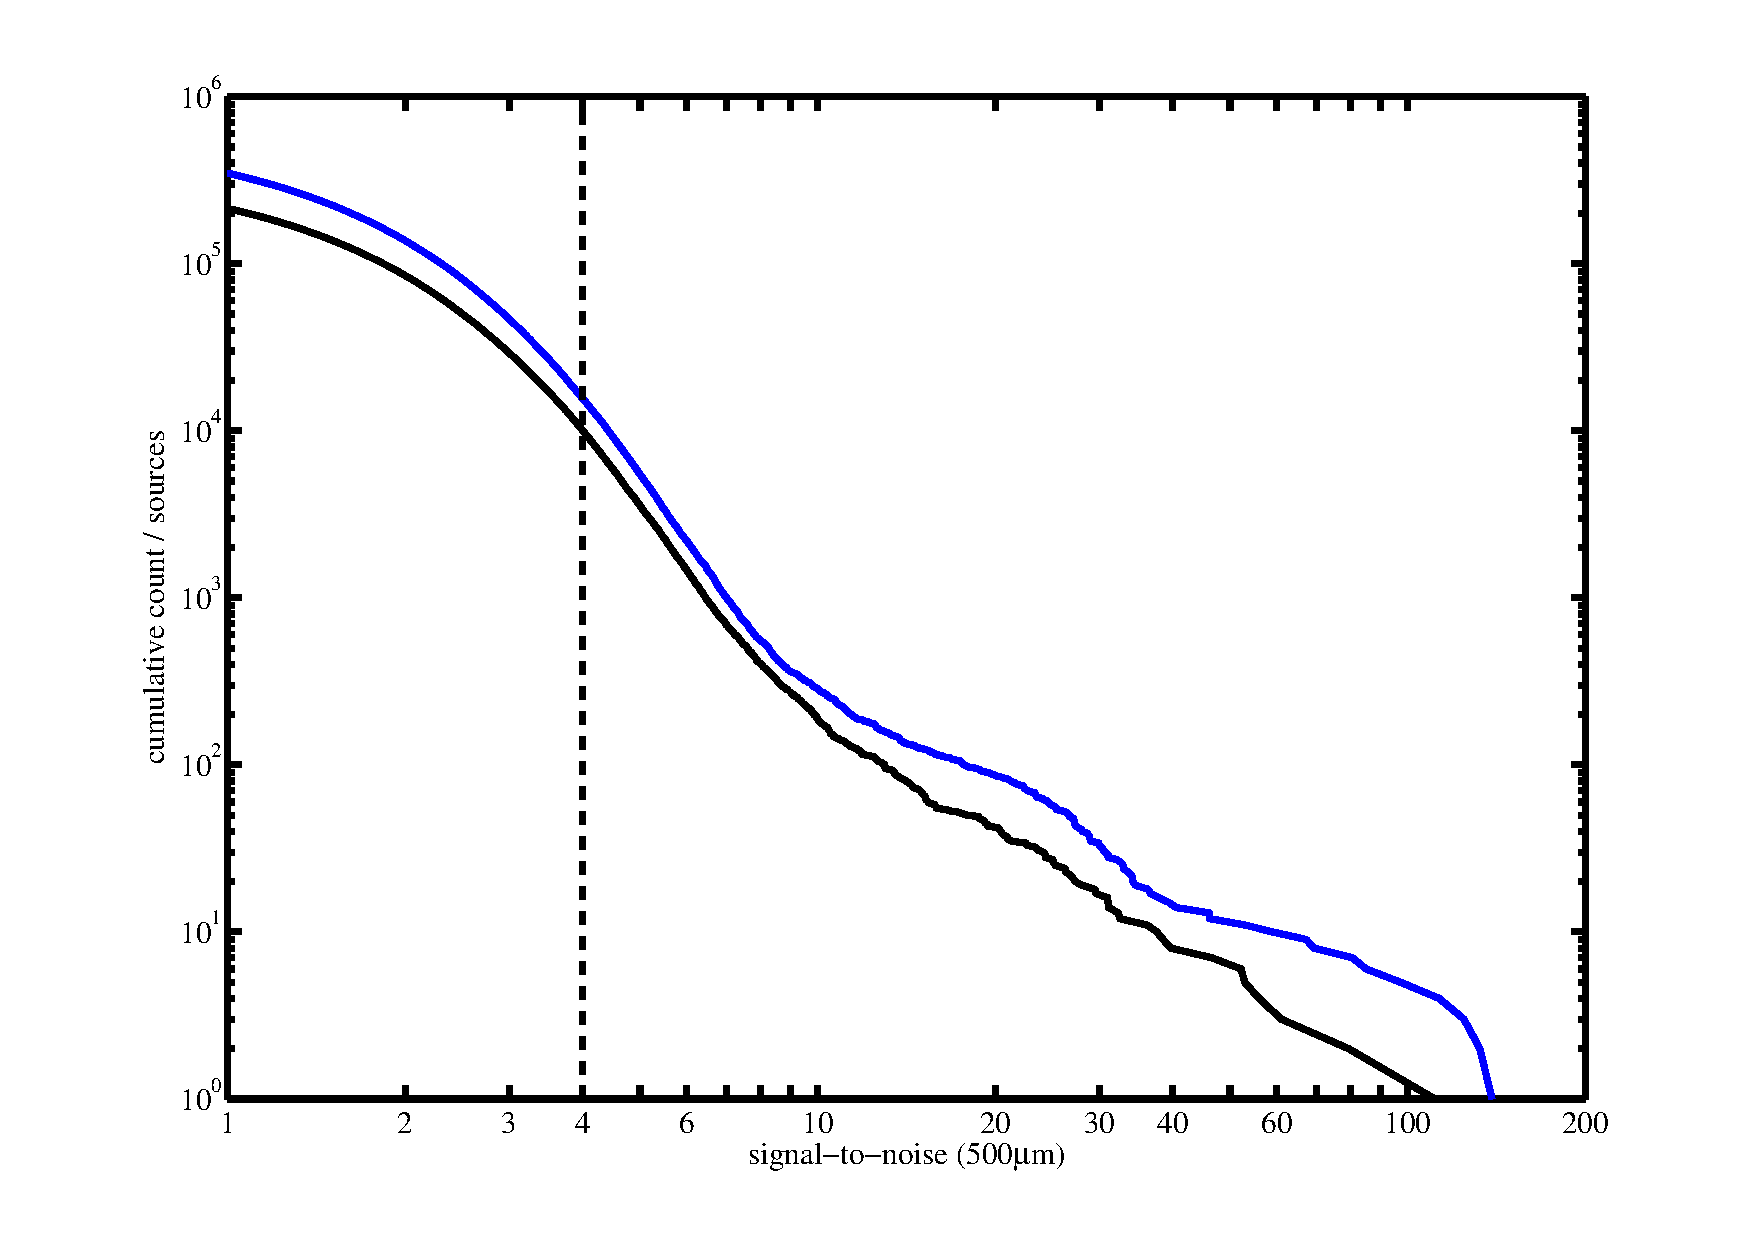
\includegraphics[width=0.42\textwidth,clip,trim={0 9mm 0mm 16mm}]{cum_sn_500.pdf}
 \caption{\protect\label{fig_sn} The cumulative number of sources as a function
   of signal-to-noise at  100\mic, 160\mic, 2250\mic, 350\mic and 500\mic}
\end{figure}

\subsection{Colour corrections and flux calibration}

The width of the SPIRE filters means that both the size of the
PSF and the power detected by SPIRE depend on the
the spectral energy distribution of the source.
The SPIRE data-reduction pipeline and ultimately our flux
densities are based on the assumption that
the flux densitiy of a
source
varies with frequency as $\nu^{-1}$. 
If the user has reason to know the SED of a source, the
flux densities should be corrected using corrections
from either Table 5.7 or 5.8 from the
SPIRE handbook\footnote{\tt{http://herschel.esac.esa.int/Docs/SPIRE/spire\_handbook.pdf}}.
It is important to apply these corrections, since they can be quite
large: for a point sources with a typical dust spectrum
($T=20K$, $\beta=2$) the multiplicative correction
is 0.96, 0.94 and 0.90 at 250, 350 and 500 $\mu$m, respectively.

As with SPIRE, the PACS flux densities are also based on the
assumption that flux density of the source is proportional to $\nu^{-1}$, and
a correction is required for sources which follow a different SED. The
required corrections are described in the PACS Colour-Correction
document\footnote{\tt{http://herschel.esac.esa.int/twiki/pub/Public/
  PacsCalibrationWeb/cc\_report\_v1.pdf}}).

On top of all other errors, there is an additional error due to the
uncertain photometric calibration of {\it Herschel}. As in V16, we assume
conservative calibration errors of 5.5\% for the three SPIRE wavebands
and 7\% for PACS (see V16 for more details).

\section{The Catalogues}

We included all sources in the catalogues if they were detected
at at least 4$\sigma$ in one or more of the three SPIRE bands: 250,
350 and 500 $\mu$m.
We eliminated all sources from the original list of point sources produced
by MADX if they fell within the aperture of an extended source. All of the H-ATLAS
fields were observed at least twice, making it possible to search for moving sources
such as asteroids. We found 9 asteroids in the GAMA fields (V16), eliminating these
from the final catalogue. We carried out the same search for the NGP and SGP but found
no moving objects.

\begin{figure*} %4
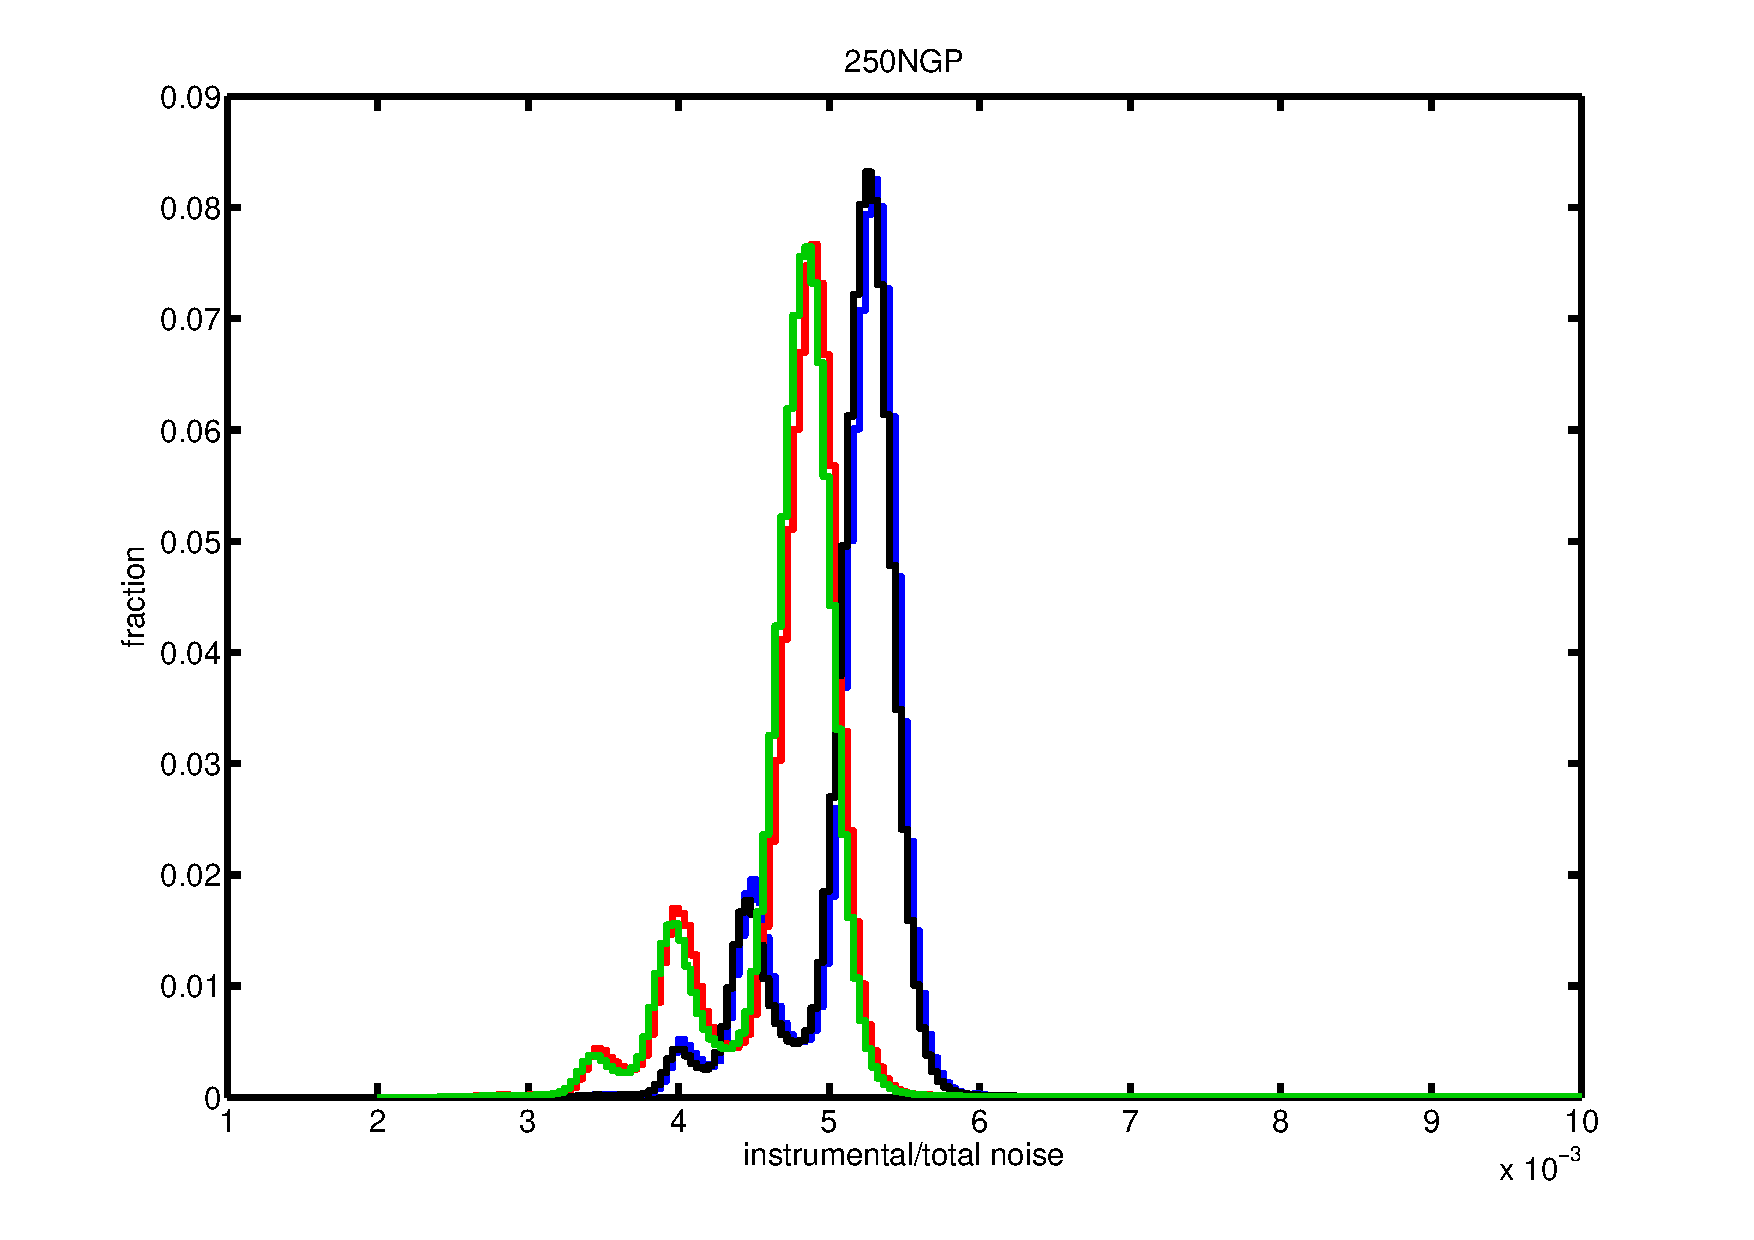
\includegraphics[width=0.3\textwidth]{flux_noise_250NGP.pdf}
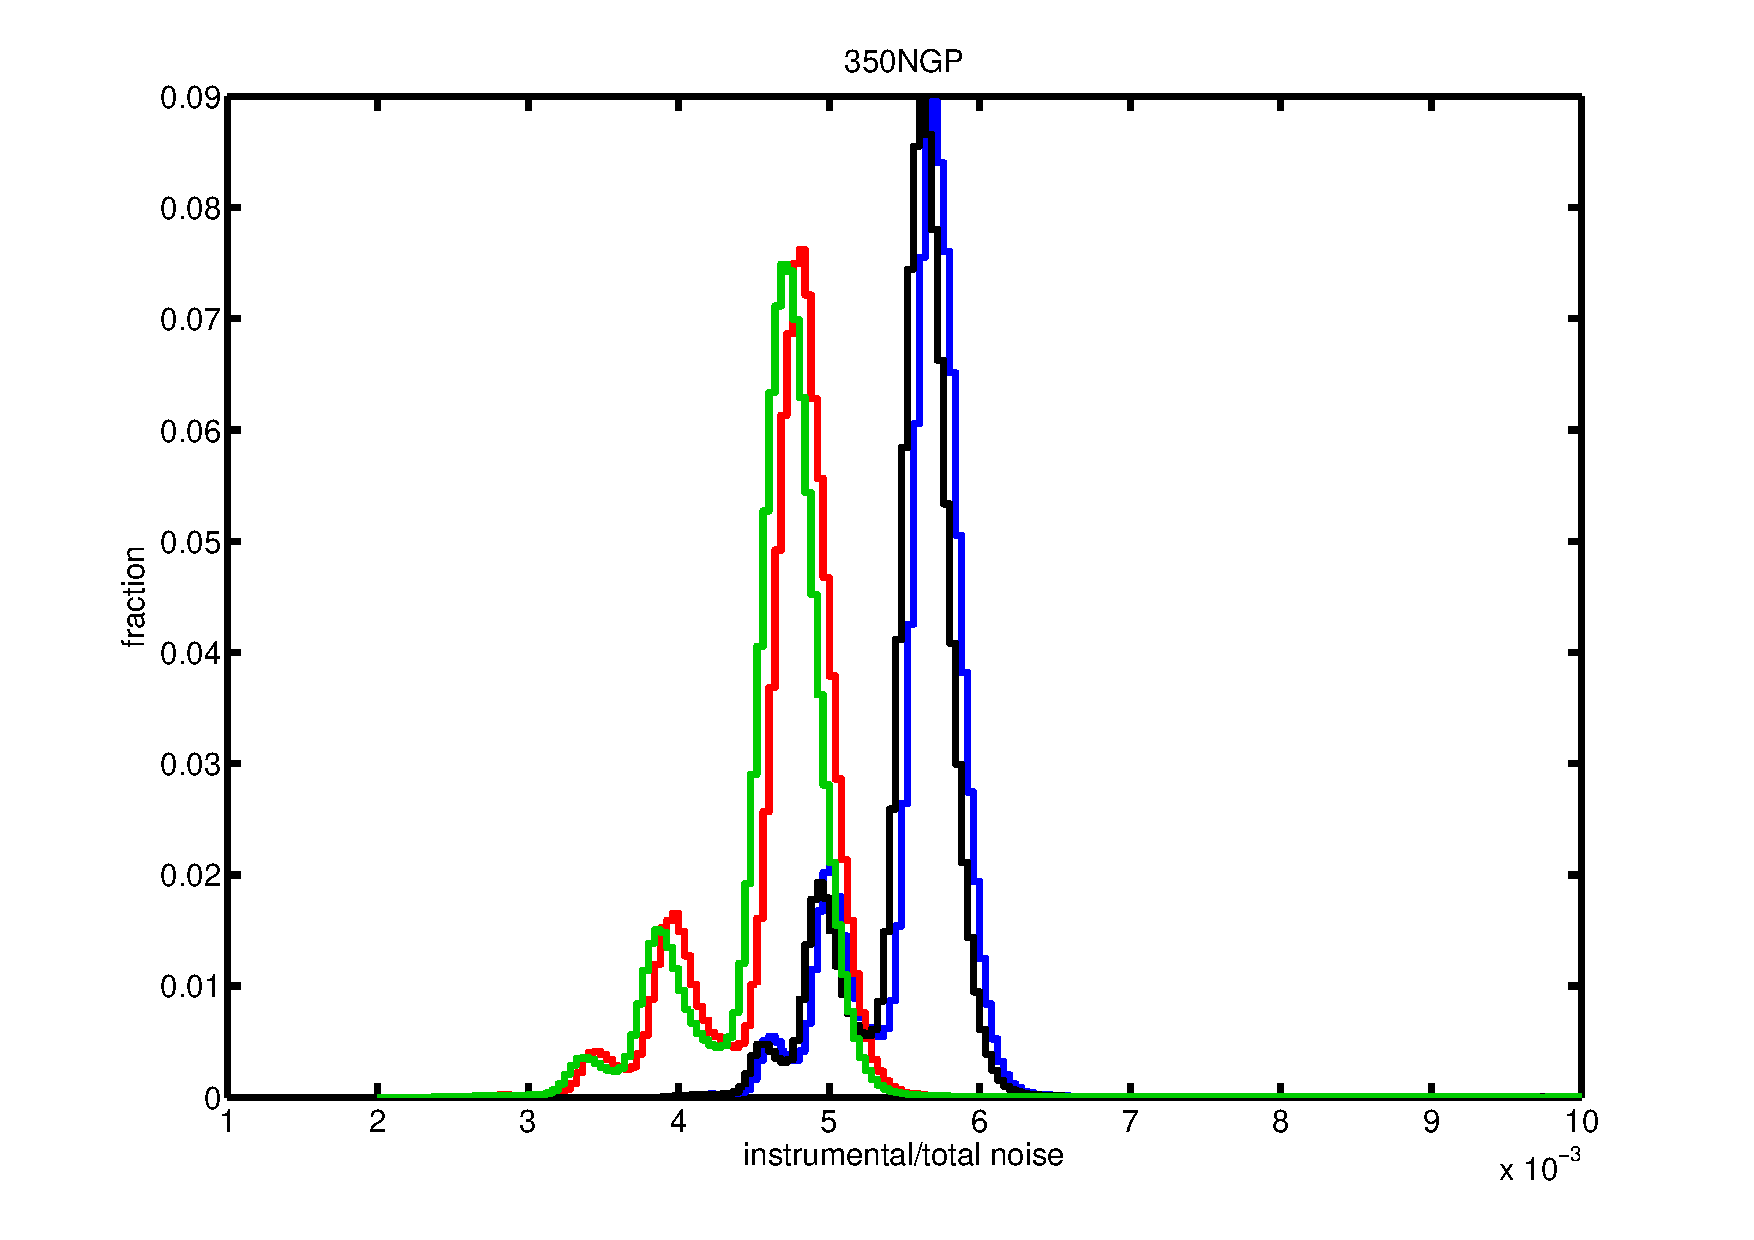
\includegraphics[width=0.3\textwidth]{flux_noise_350NGP.pdf}
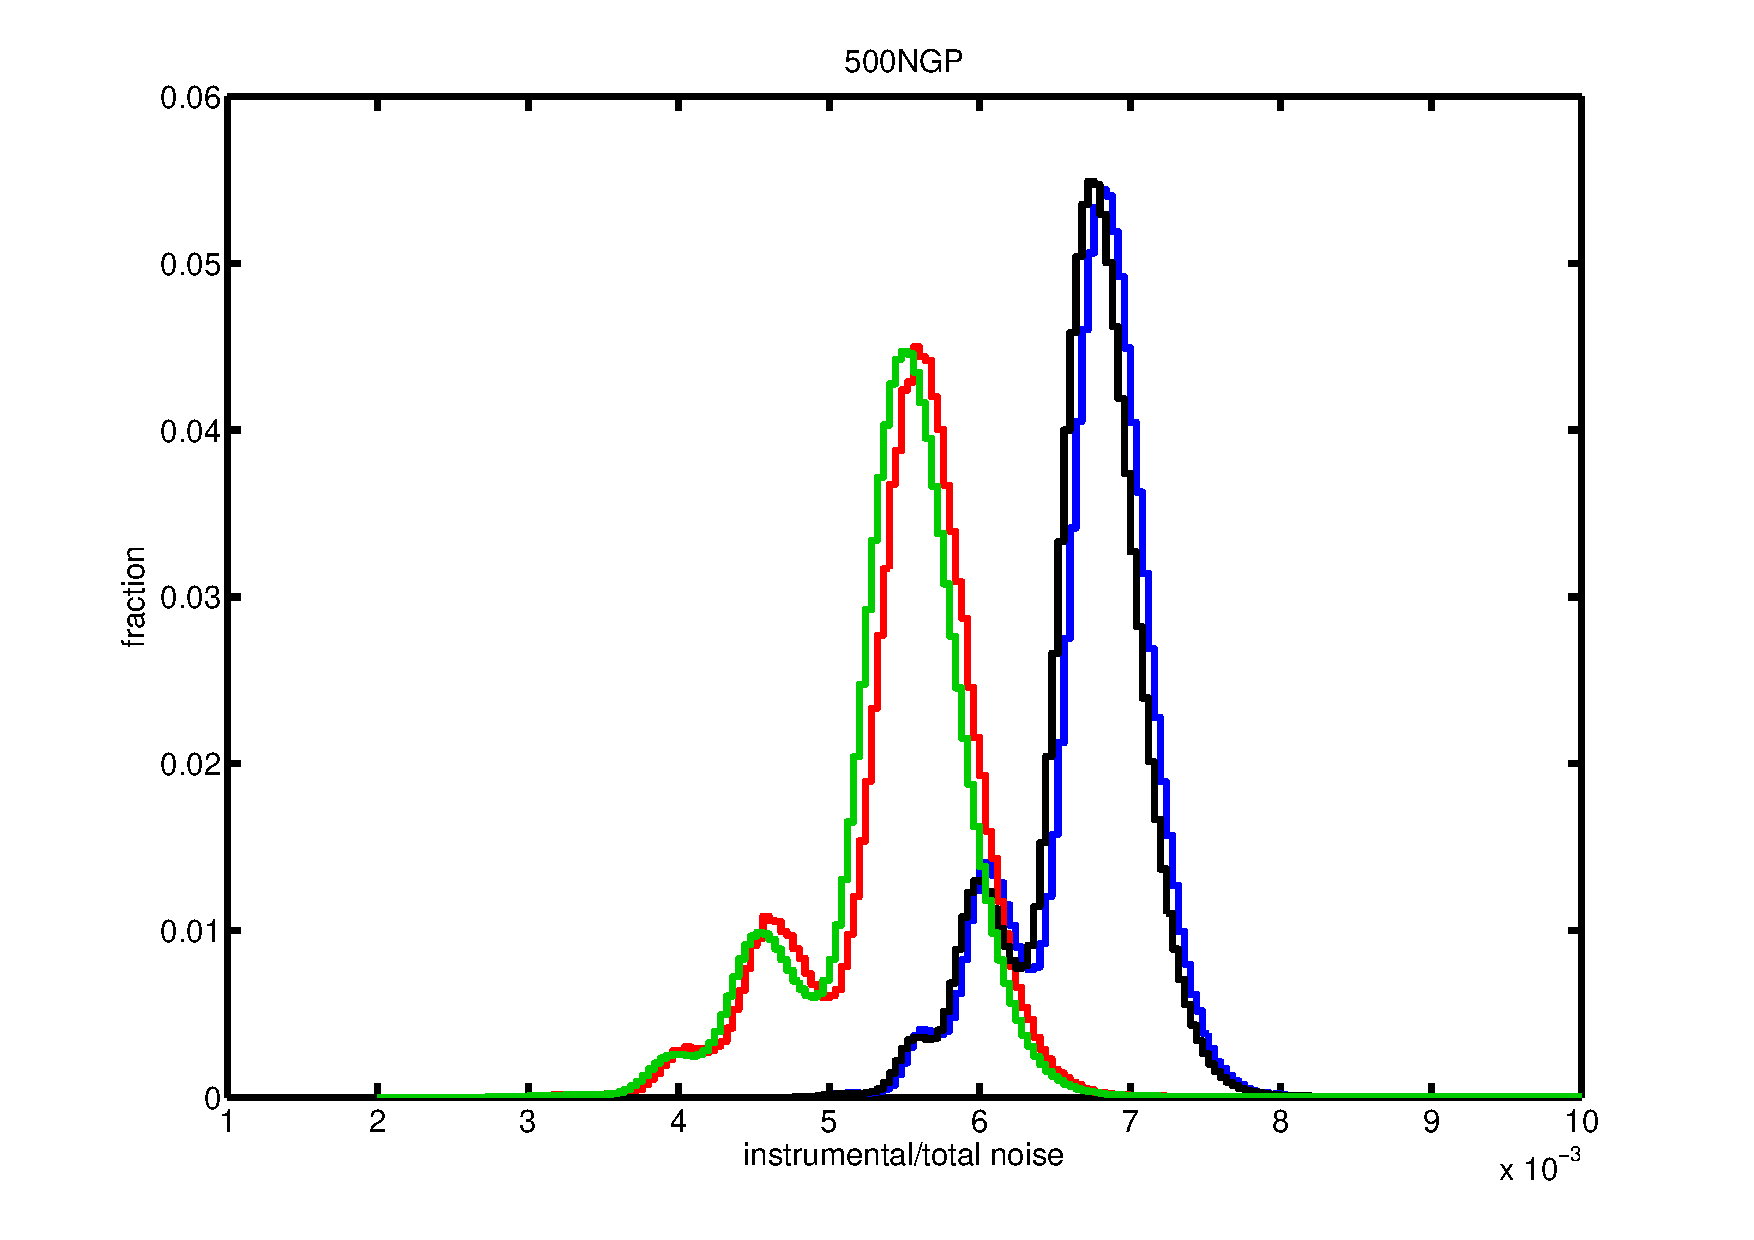
\includegraphics[width=0.3\textwidth]{flux_noise_500NGP.pdf}
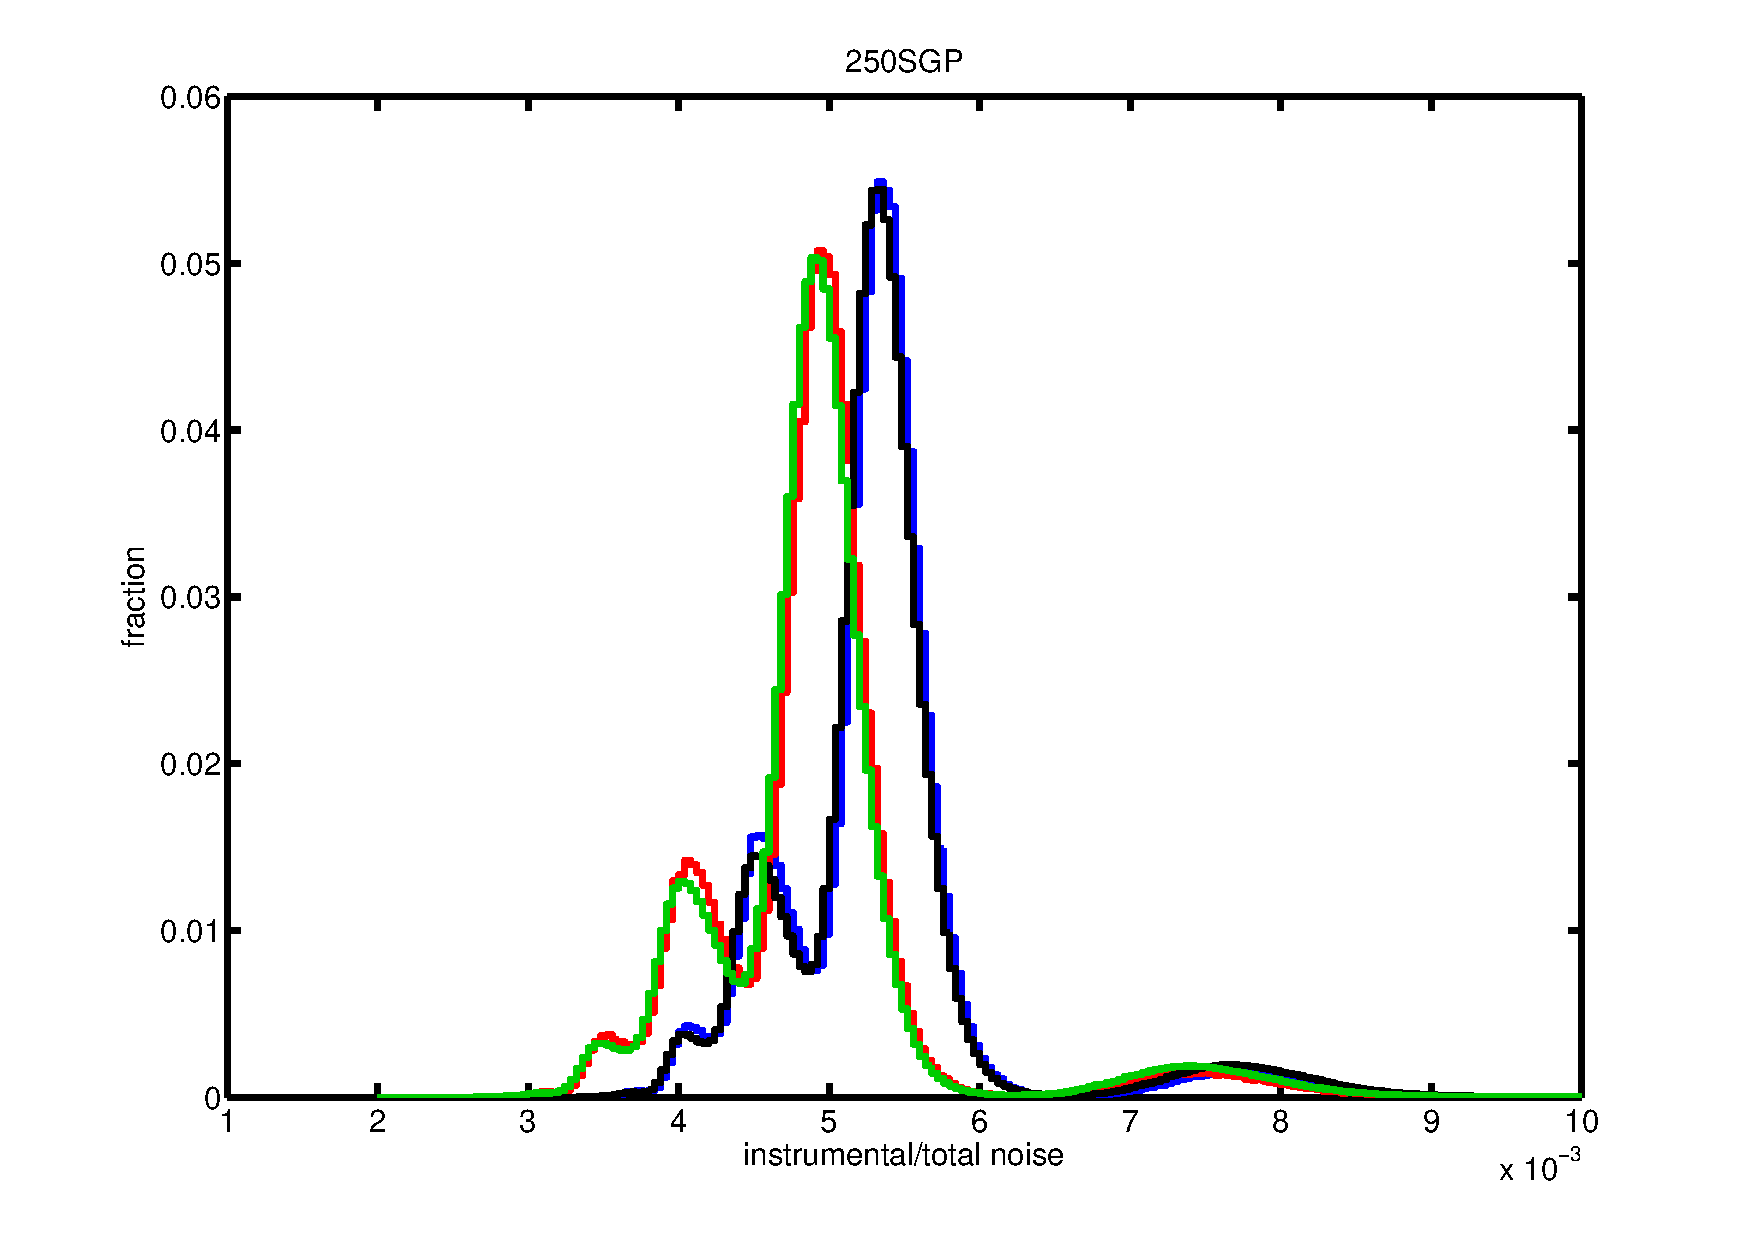
\includegraphics[width=0.3\textwidth]{flux_noise_250SGP.pdf}
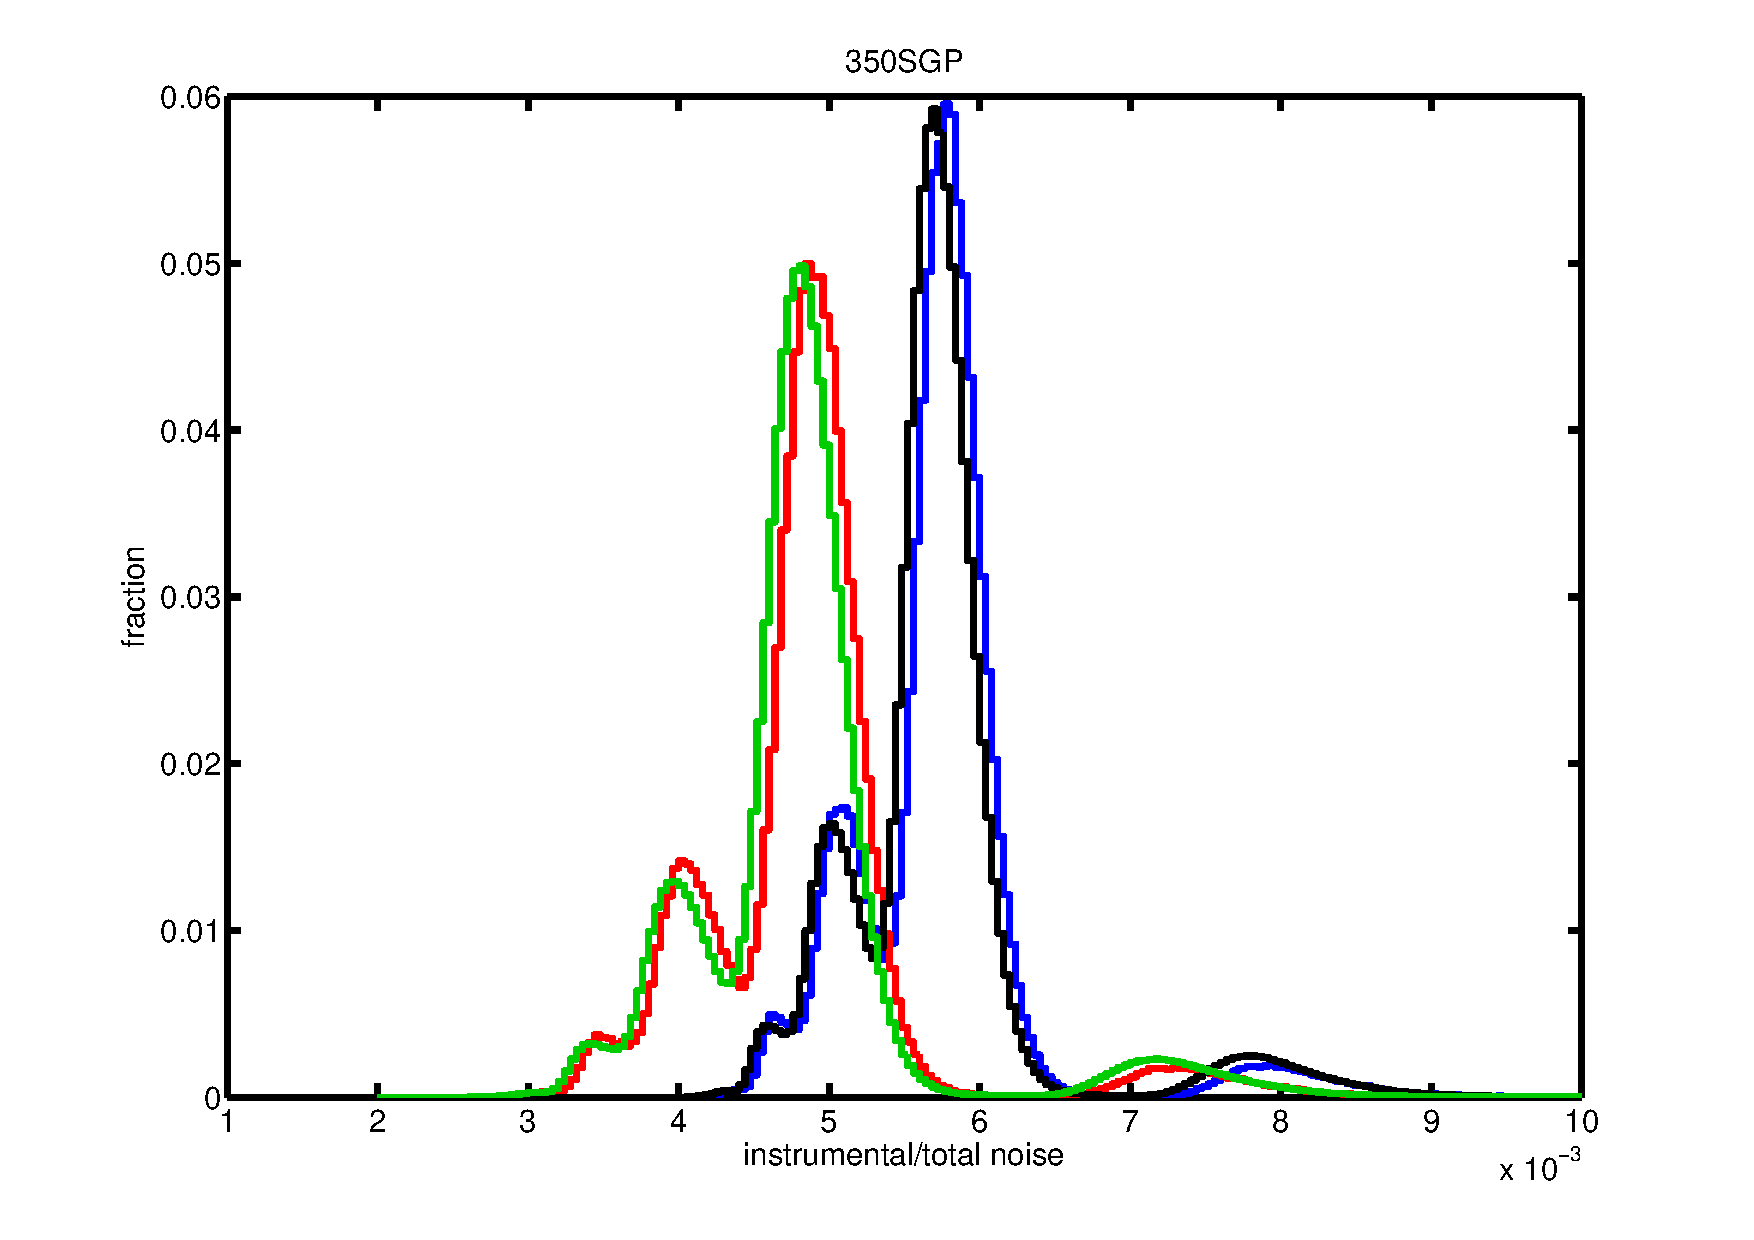
\includegraphics[width=0.3\textwidth]{flux_noise_350SGP.pdf}
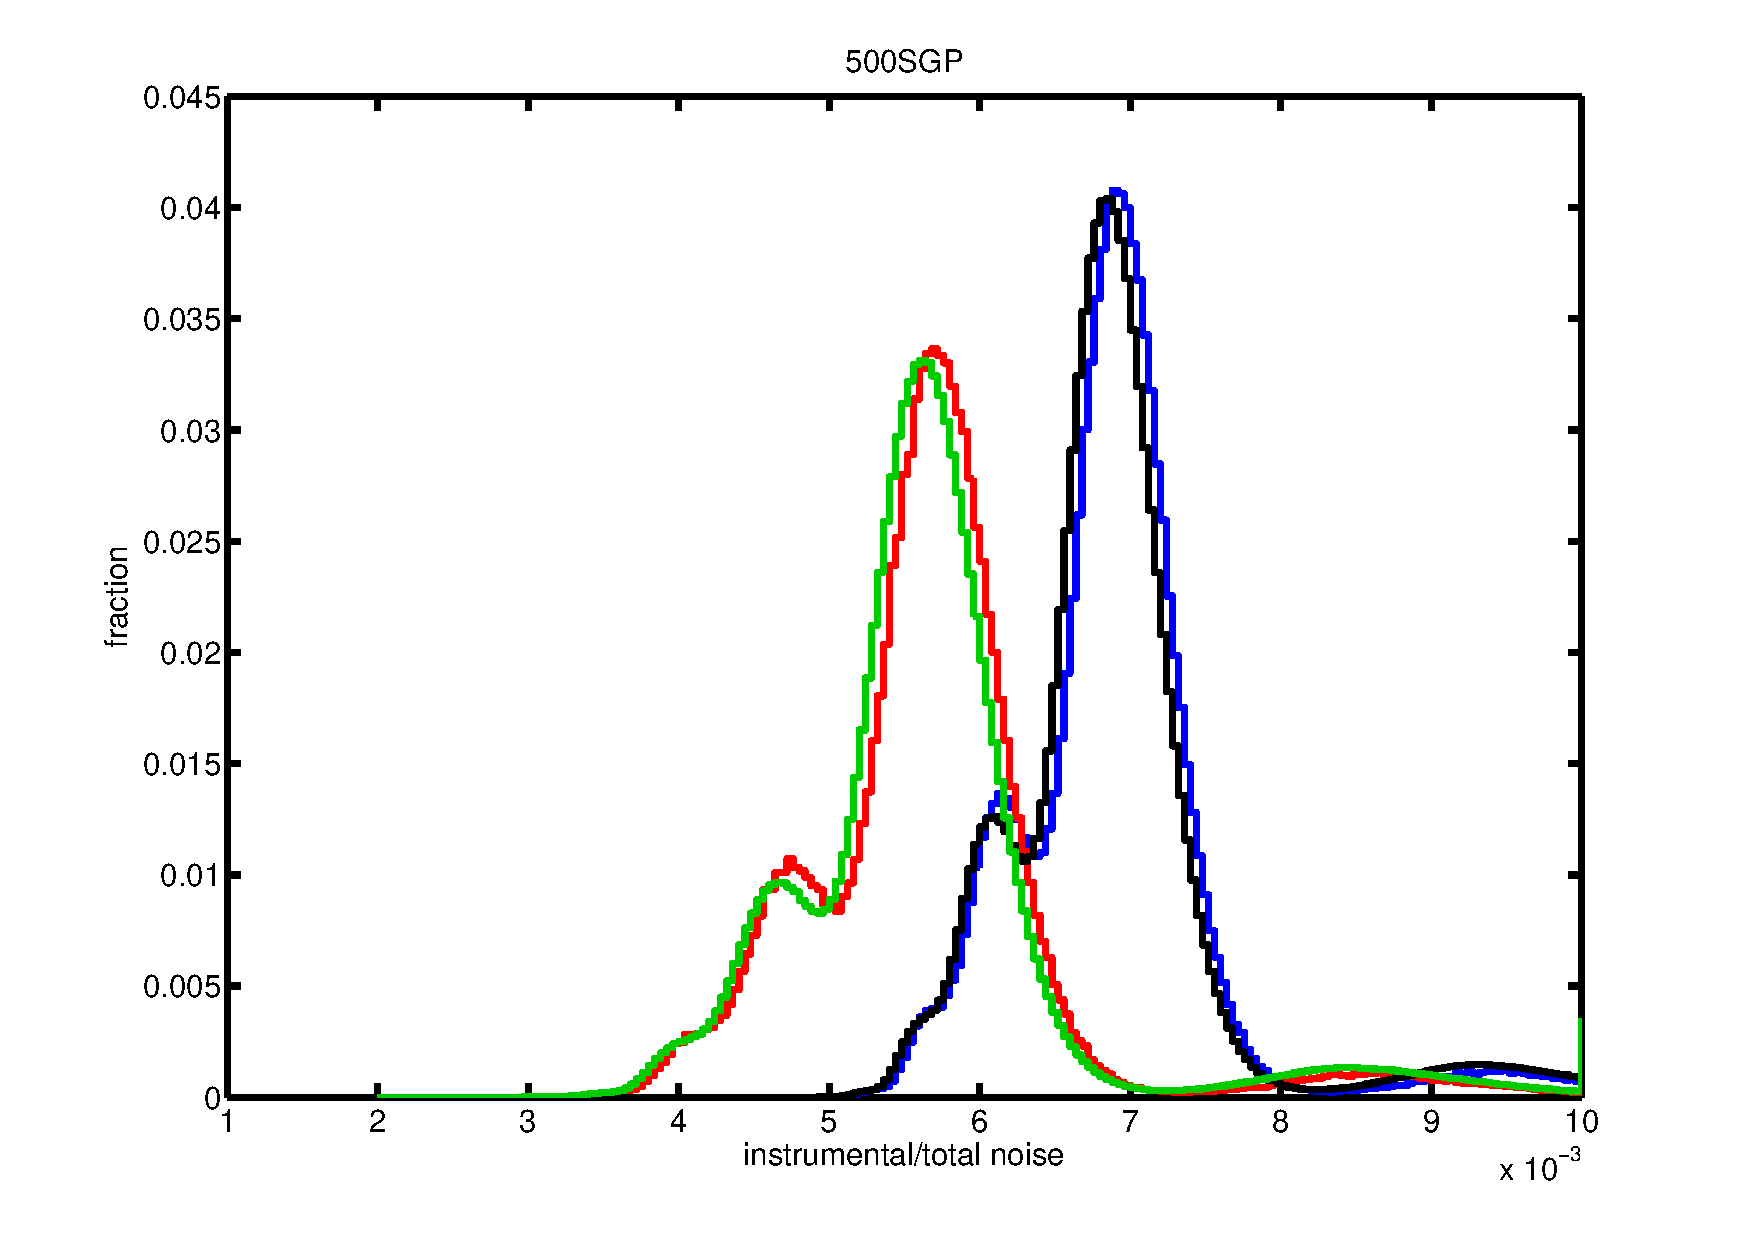
\includegraphics[width=0.3\textwidth]{flux_noise_500SGP.pdf}
\caption{The distribution of instrumental and total noise
for
  the 250\mic, 350\mic and 500\mic fluxes bands
for the NGP and SGP fields.
  Green shows the instrumental noise and
black the total noise for all pixels; red shows the
instrumental noise and blue the total noise at the positions of all sources.
The multiple peaks are the results of our tiling strategy. The
main peak corresponds to the large fraction of the survey
area that was covered by two individual {\it Herschel}
observations (S17). The smaller peaks correspond to
the smaller fraction of the survey area that was either
covered by more than two observations or, in the case of one
end of the SGP (S17), a
single observation (the small peak at the right in the bottom
panels.}
\label{fig_noises}
\end{figure*}

The sources in the final catalogues are almost all extragalactic sources. We carried out
a search for clusters of sources in all the H-ATLAS fields (Eales et al. in preparation).
In the GAMA9 field, we found several clusters of sources that are likely to
be clusters of prestellar cores, implying 
that the catalogue for this field
is likely to contain a few tens of Galactic sources.
However, we found no similar clusters in the other fields and the
GAMA9 field is at a much lower Galactic latitude than the other
fields. Prestellar cores are therefore likely to be a very minor contaminant to the
catalogues for these fields. There are a few debris disks and AGB stars
in the catalogues, 
and an incomplete list is given in Table 1.
However, well over 99\% of the sources are extragalactic. The extragalactic
sources range from nearby galaxies, such as the spectacular galaxy, XXXX,
in the centre of the SGP to galaxies up to a redshift of $\simeq$6 (Fudamoto
et al. 2017).

\subsection{The statistics of the catalogues}

The catalogue for the NGP contains 118,986 sources, of which 112,074 were detected
at $>4\sigma$ at 250 $\mu$m, 46,872 at $>4\sigma$ at 350 $\mu$m and 10,369 at
$>4\sigma$ at 500 $\mu$m. The effective sensitivity of the PACS images was
much less, but the catalogues contain flux-density measurements at 100 $\mu$m and
160 $\mu$m for all the sources in the catalogue. 4,207  sources were detected
at $>3\sigma$ at 100 $\mu$m and 6,342 sources were detected at 
$>3\sigma$ at 160 $\mu$m.

The catalogue for the SGP contains XXXX sources, of which XXXX  were detected
at $>4\sigma$ at 250 $\mu$m, XXXX at $>4\sigma$ at 350 $\mu$m and XXXX  at
$>4\sigma$ at 500 $\mu$m. 
XXX sources were detected
at $>3\sigma$ at 100 $\mu$m and XXXX sources were detected at 
$>3\sigma$ at 160 $\mu$m.

\begin{figure} %5
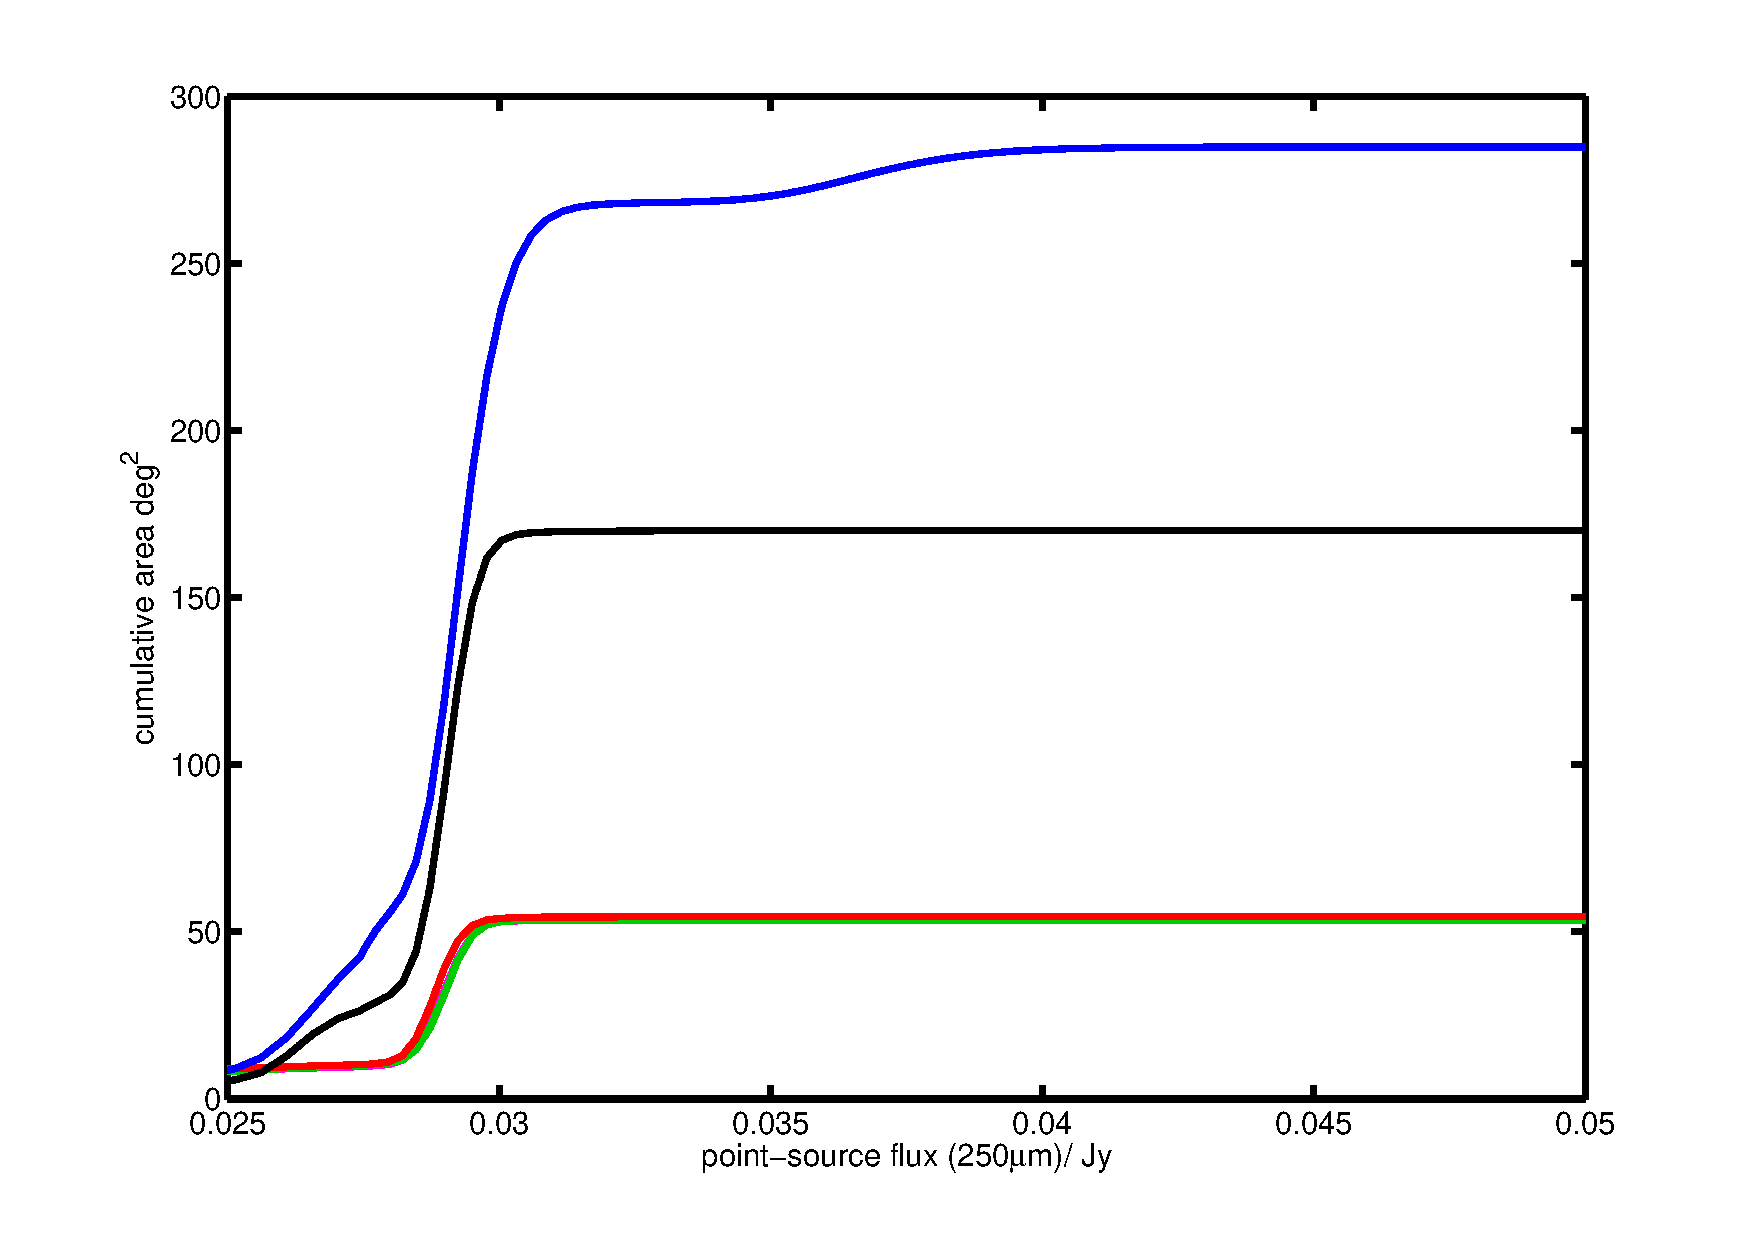
\includegraphics[width=0.5\textwidth]{flux_area_250.pdf}
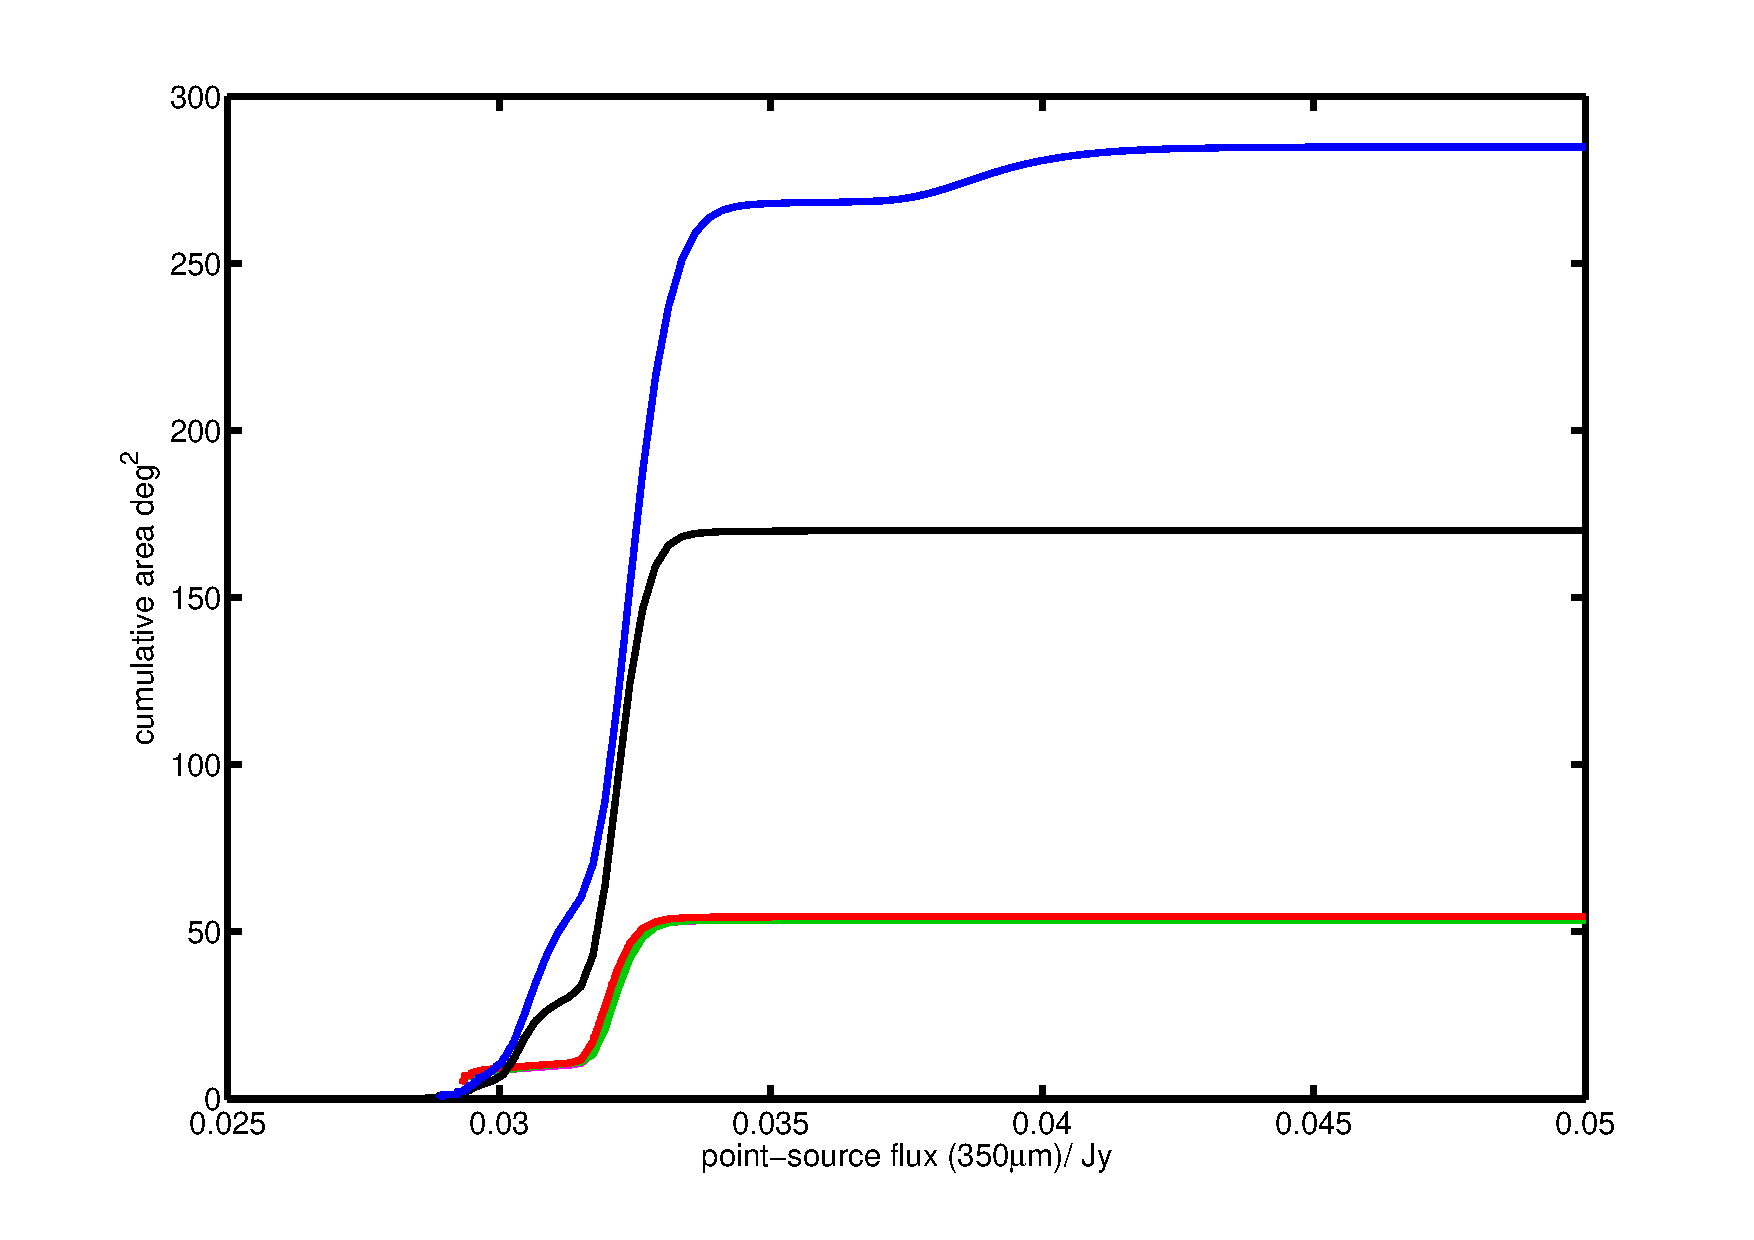
\includegraphics[width=0.5\textwidth]{flux_area_350.pdf}
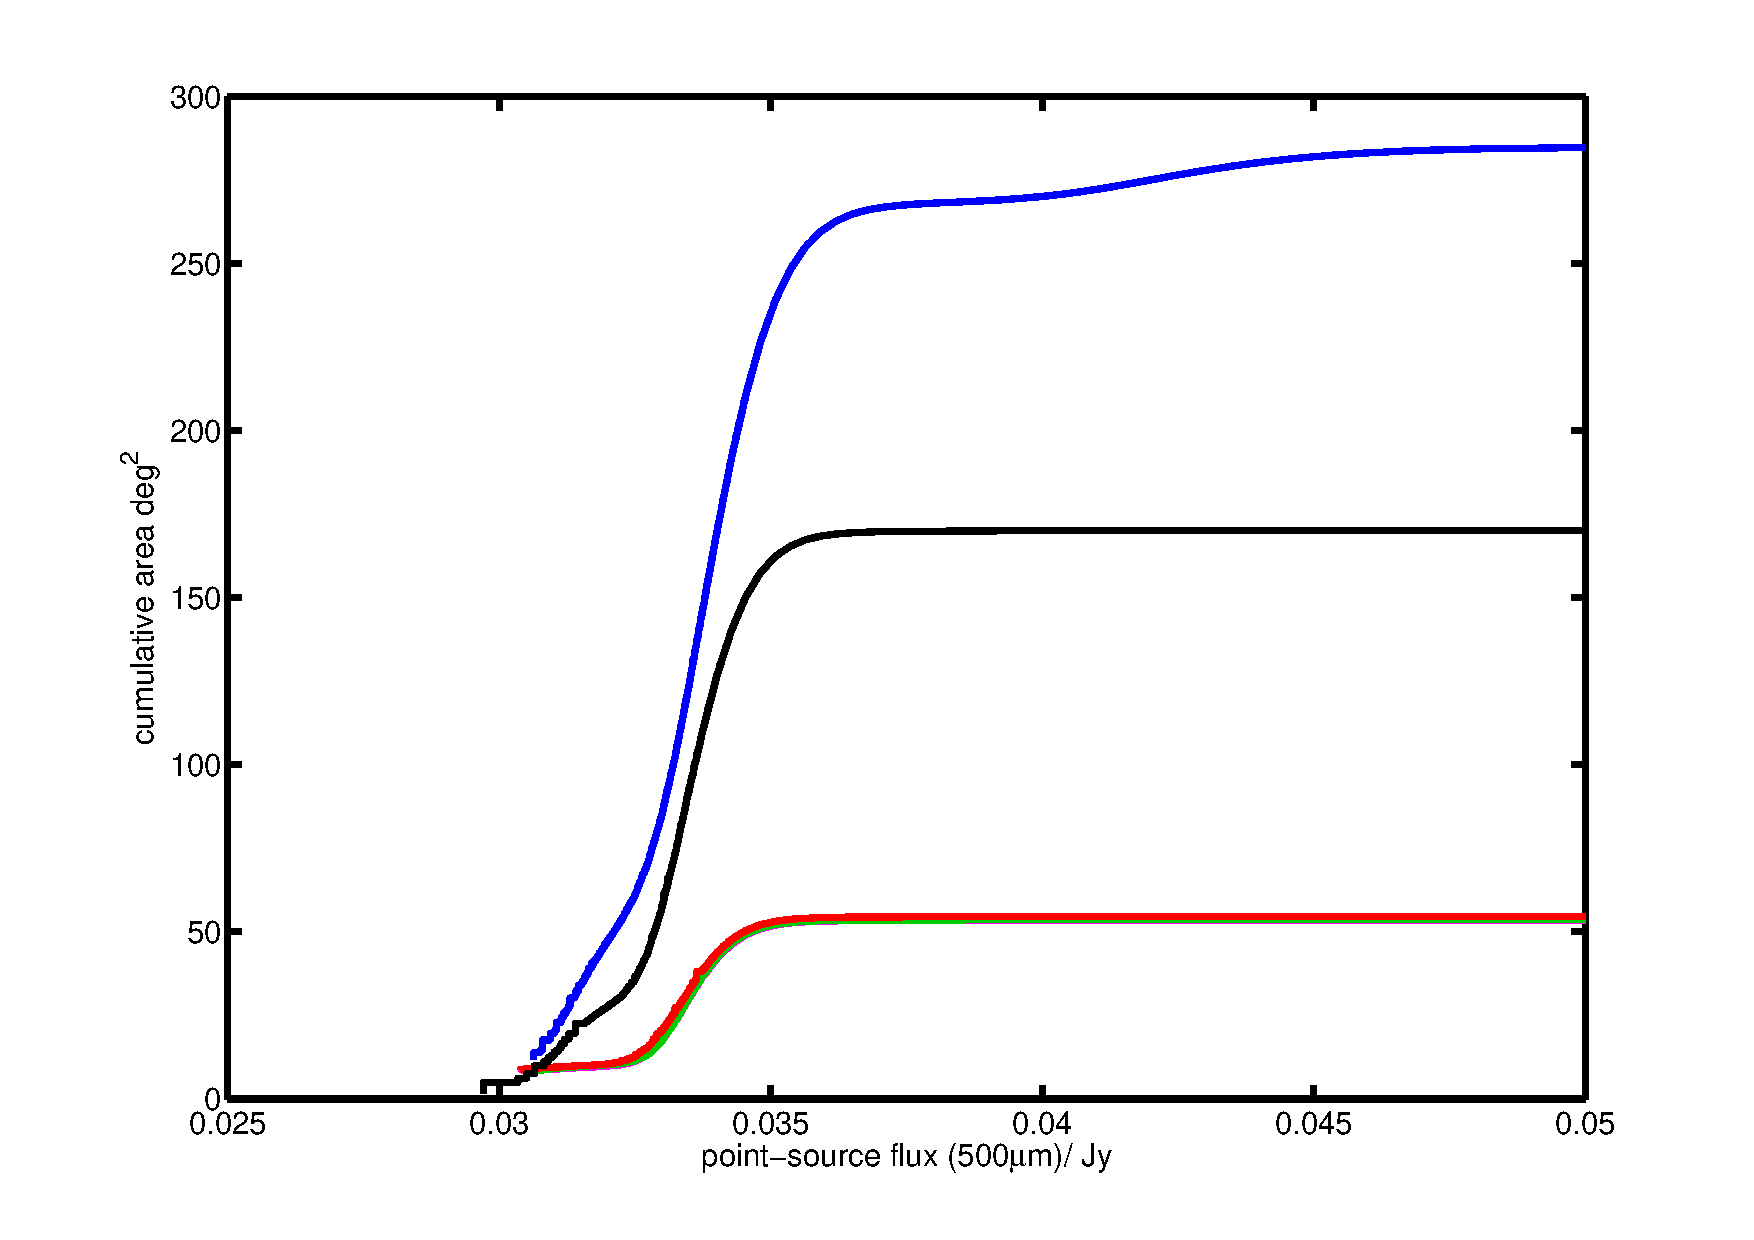
\includegraphics[width=0.5\textwidth]{flux_area_500.pdf}
\caption{The
relationship between area and 4$\sigma$ flux-density limit
for the
  H-ATLAS fields: NGP - black; SGP - blue; GAMA9 - magenta; GAMA12 - green;
  GAMA15 - cyan.  The more sensitive areas correspond to the
tile overlaps in each field.
The westerly end of SGP has only a single SPIRE observation,
which explains the kink at high flux densities
in the blue line in the panels.}

\label{fig_areas}
\end{figure}

The observed number of sources as  function of flux in the PACS and
SPIRES bands is shown in Figure~\ref{fig_cum_flux}. 
Note that this is the observed flux in the catalogue, before any
corrections are made for source SED (Section 3.3) or `flux boosting'
(Section 4.3), which are necessary
before the flux densities are compared with model predictions.
The cumulative number of sources as a function of signal-to-noise in
the 250\mic detection band is shown in Figure 4.

Because of our strategy of creating the H-ATLAS survey
from overlapping tiles (S17),
the instrumental noise varies over the maps.
Figure 5 shows histograms of instrumental noise and total noise
(instrumental noise plus confusion noise) for all pixels
and at the positions of all sources.
The large peak corresponds to the large fraction of the
survey area that was covered by two observations, with the
other peaks corresponding to the smaller area covered by
either more observations or, for one area of the SGP, a single
observation (S17).

The variation of noise across the maps means that 
4$\sigma$ flux-density limit varies over the fields.
Figure 6 shows the relationship between 
area and flux-density limit
for each of the H-ATLAS fields, including the GAMA fields.

\subsection{Positional Accuracy}

V16 carried out extensive simulations to ivestigate the
accuracy of the H-ATLAS catalogues by injecting
artificial sources on to the GAMA images, and then using MADX to detect the
sources and measure their flux densities and positions. The results
of these `in-out' simulations apply to the NGP and SGP catalogues, which were
produced using almost exactly the same methods.

We investigated the accuracy of the source positions
in two ways: (1) by looking at the positional offsets
between the {\it Herschel} sources and galaxies found
on optical images; (2) from the in-out simulations.
Bourne et al. (2016) and F17 describe the details of the first method,
which takes account of the clustering of the galaxies in the optical
catalogue and the PSF of the {\it Herschel} observations.
We also use the positions of the galaxies to correct the
astrometry of the individual {\it Herschel} observations, which
ties the positions of the {\it Herschel} sources
to the astrometric frame of the optical catalogue (S17).

In the case of the NGP, we applied this method using
the galaxies found on the SDSS r-band images (F17), which
thus ultimately ties the {\it Herschel} positions to
the SDSS astrometric frame.
In the case of the SGP, we used the galaxies
found in the VLT Survey Telescope ATLAS (Shanks et al.
2015), which thus ultimately ties the astronometry in the
SGP to the astrometric frame of this survey.
We find that the positional error,
$\sigma_\mathrm{pos}$, varies from 1.2'' to 2.4'' as the
signal-to-noise in flux varies from 10 to 5, 
with a relationship between positional accuracy and flux density
given by
$\sigma_\mathrm{pos} =
2.4 (\mathrm{SNR}/5)^{-0.84}$.
This agrees well with the errors in the measured
positions of the
artificial sources in the in-out simulations (V16).

%\begin{figure}
%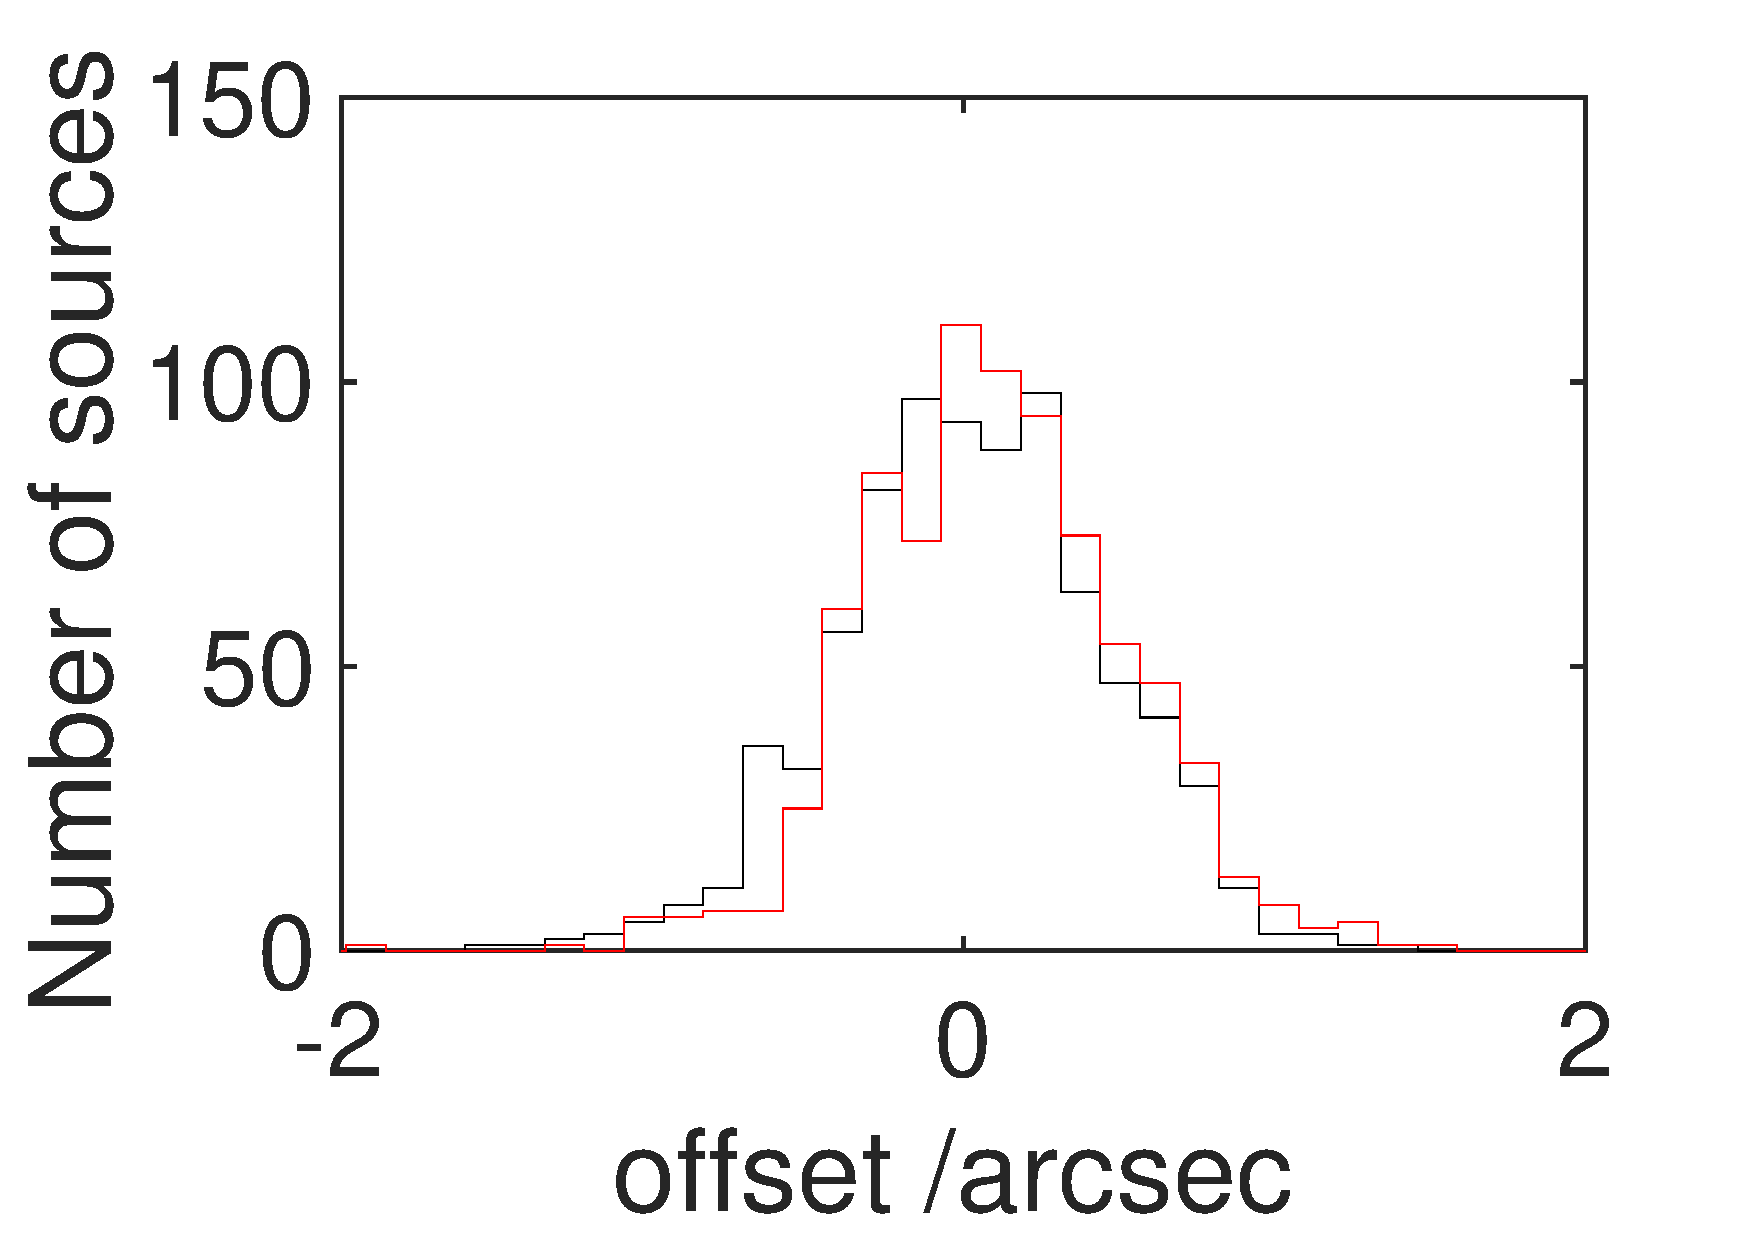
\includegraphics[scale=0.3]{ngp_pos_err_hist.pdf}
%\caption{\protect\label{fig_pos_err_hist} The distribution of
%  positional offsets between SPIRE and SDSS sources in the NGP. 
%The black histogram shows the offsets in RA, and the red line the
%offsets in DEC. 
%!!!IS this the map alignment histogram or the XID one? Which sources are included?
%}
%\end{figure}

The mean positional errors as a function of position within the NGP
and SGP fields are shown in Fig.~\ref{fig_pos_errs}. Though there are
hints of systematic variations in different part of the fields, 
these are only $\simeq$1 arcsec, less than the
quoted pointing accuracy of {\it Herschel} of
$\simeq$2 arcsec (Pilbratt et al. 2010).

\begin{figure*}
%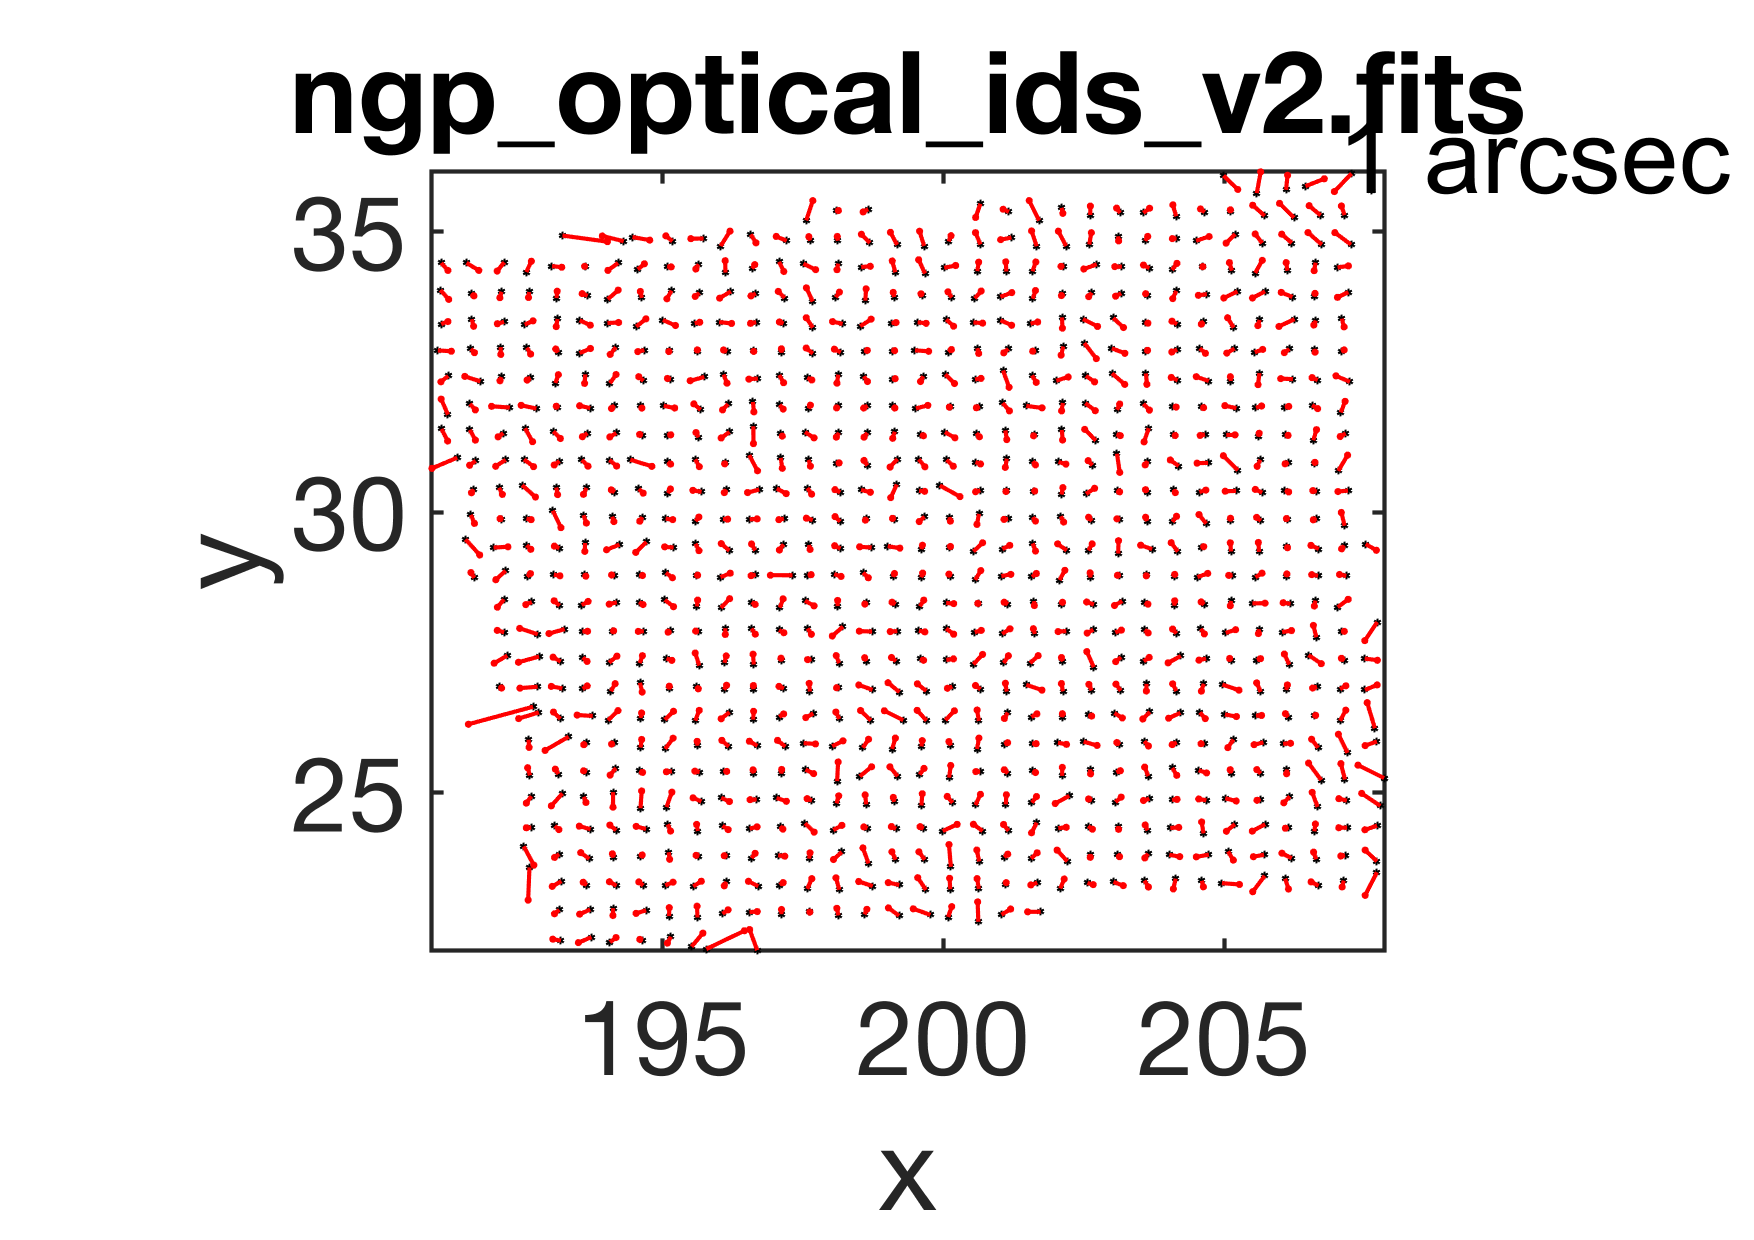
\includegraphics[scale=0.3]{ngp_posn_errors_new.pdf}
%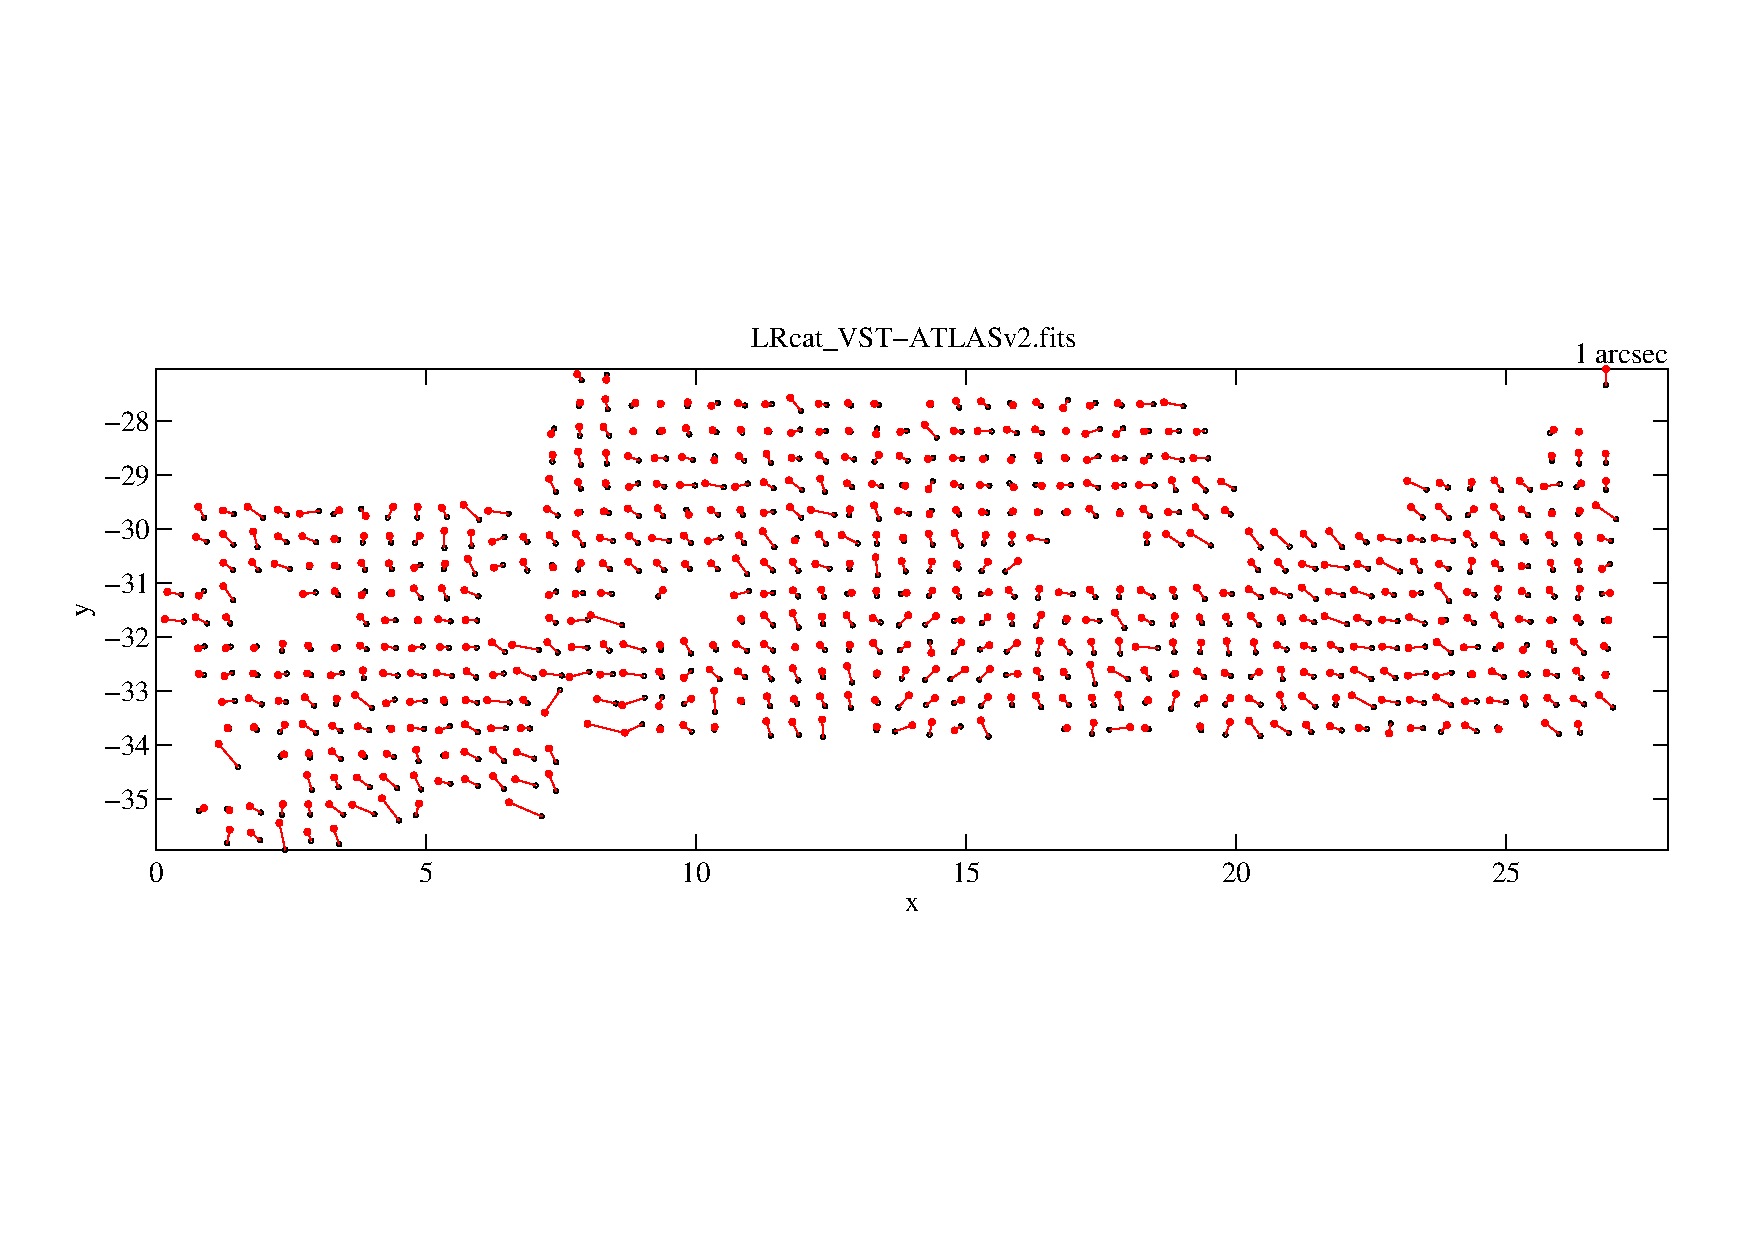
\includegraphics[scale=0.3,trim=0 45mm 0mm 45mm]{sgp_astrometry2.pdf}
%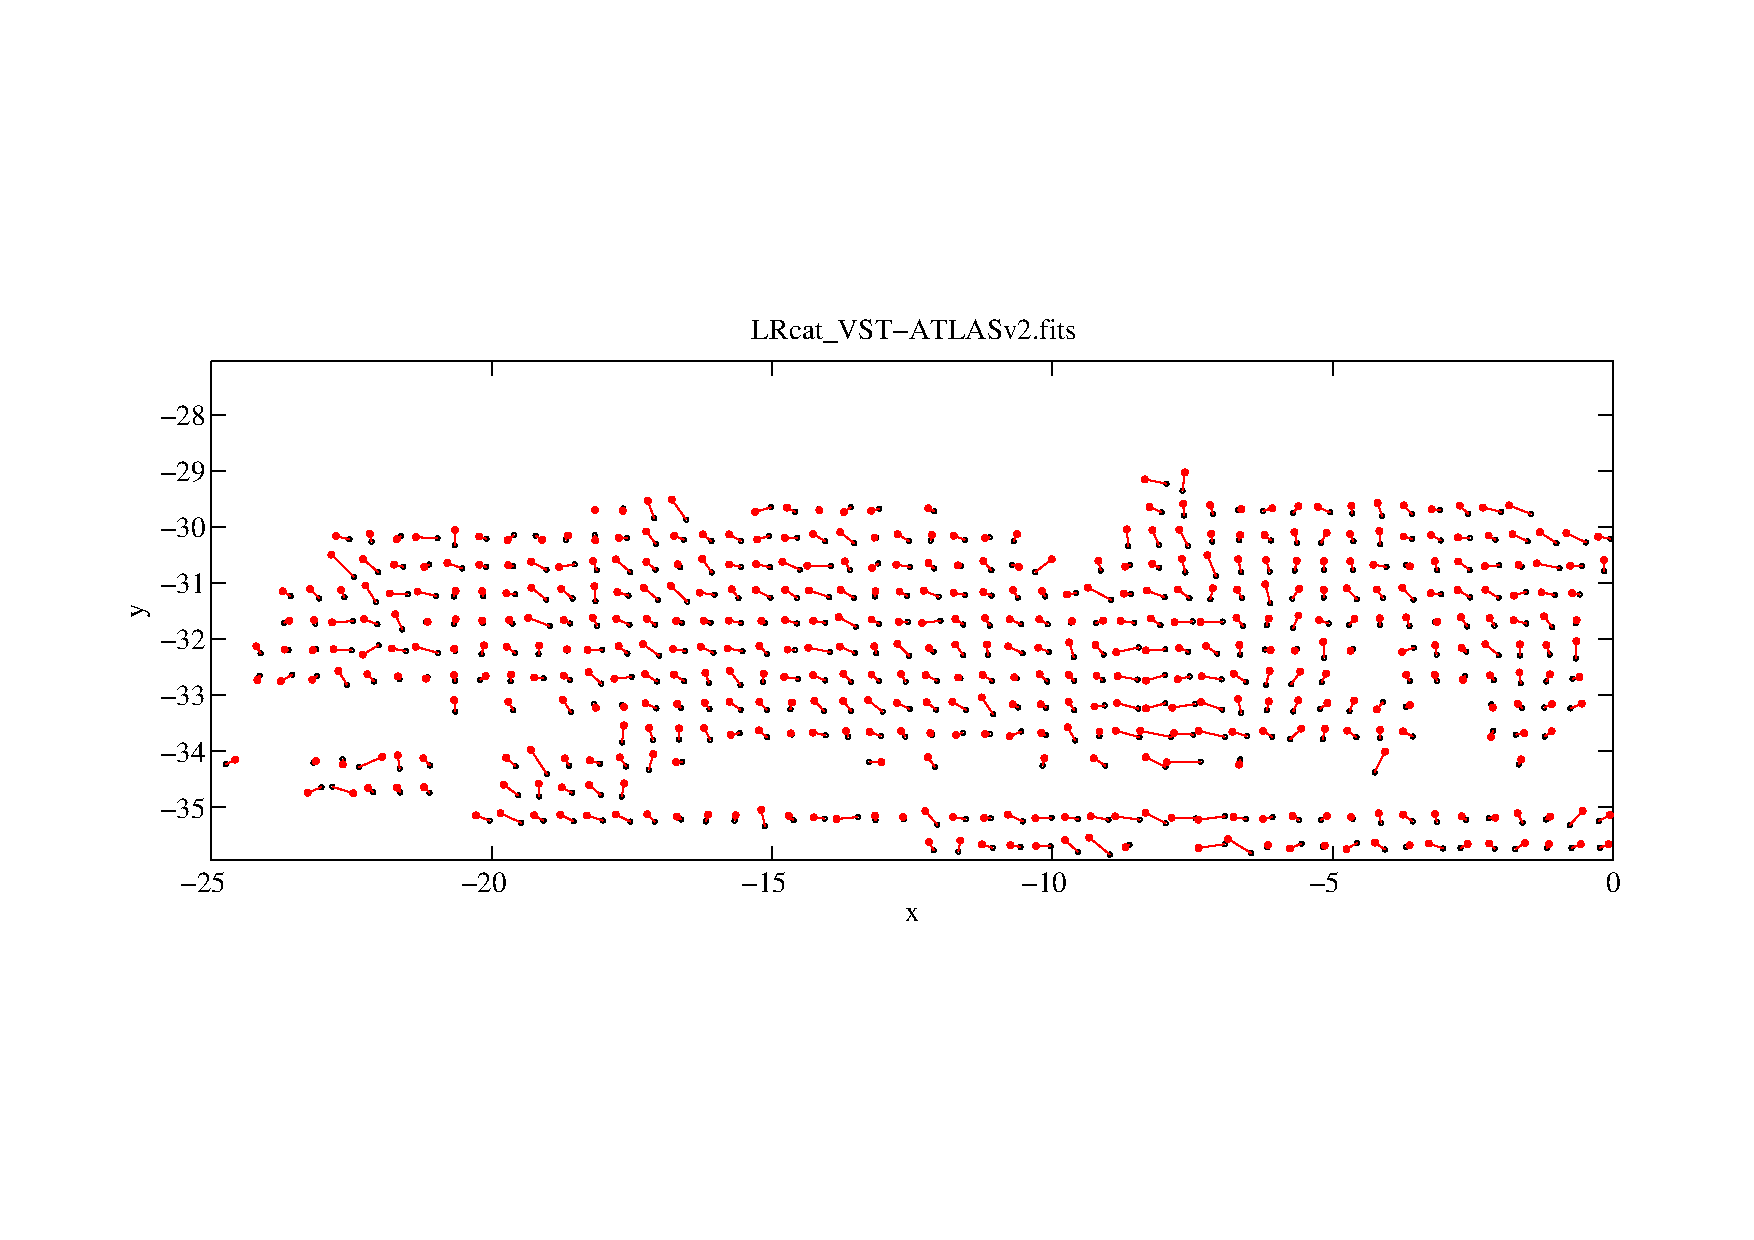
\includegraphics[scale=0.3,trim=0 45mm 0mm 45mm]{sgp_astrometry1.pdf}
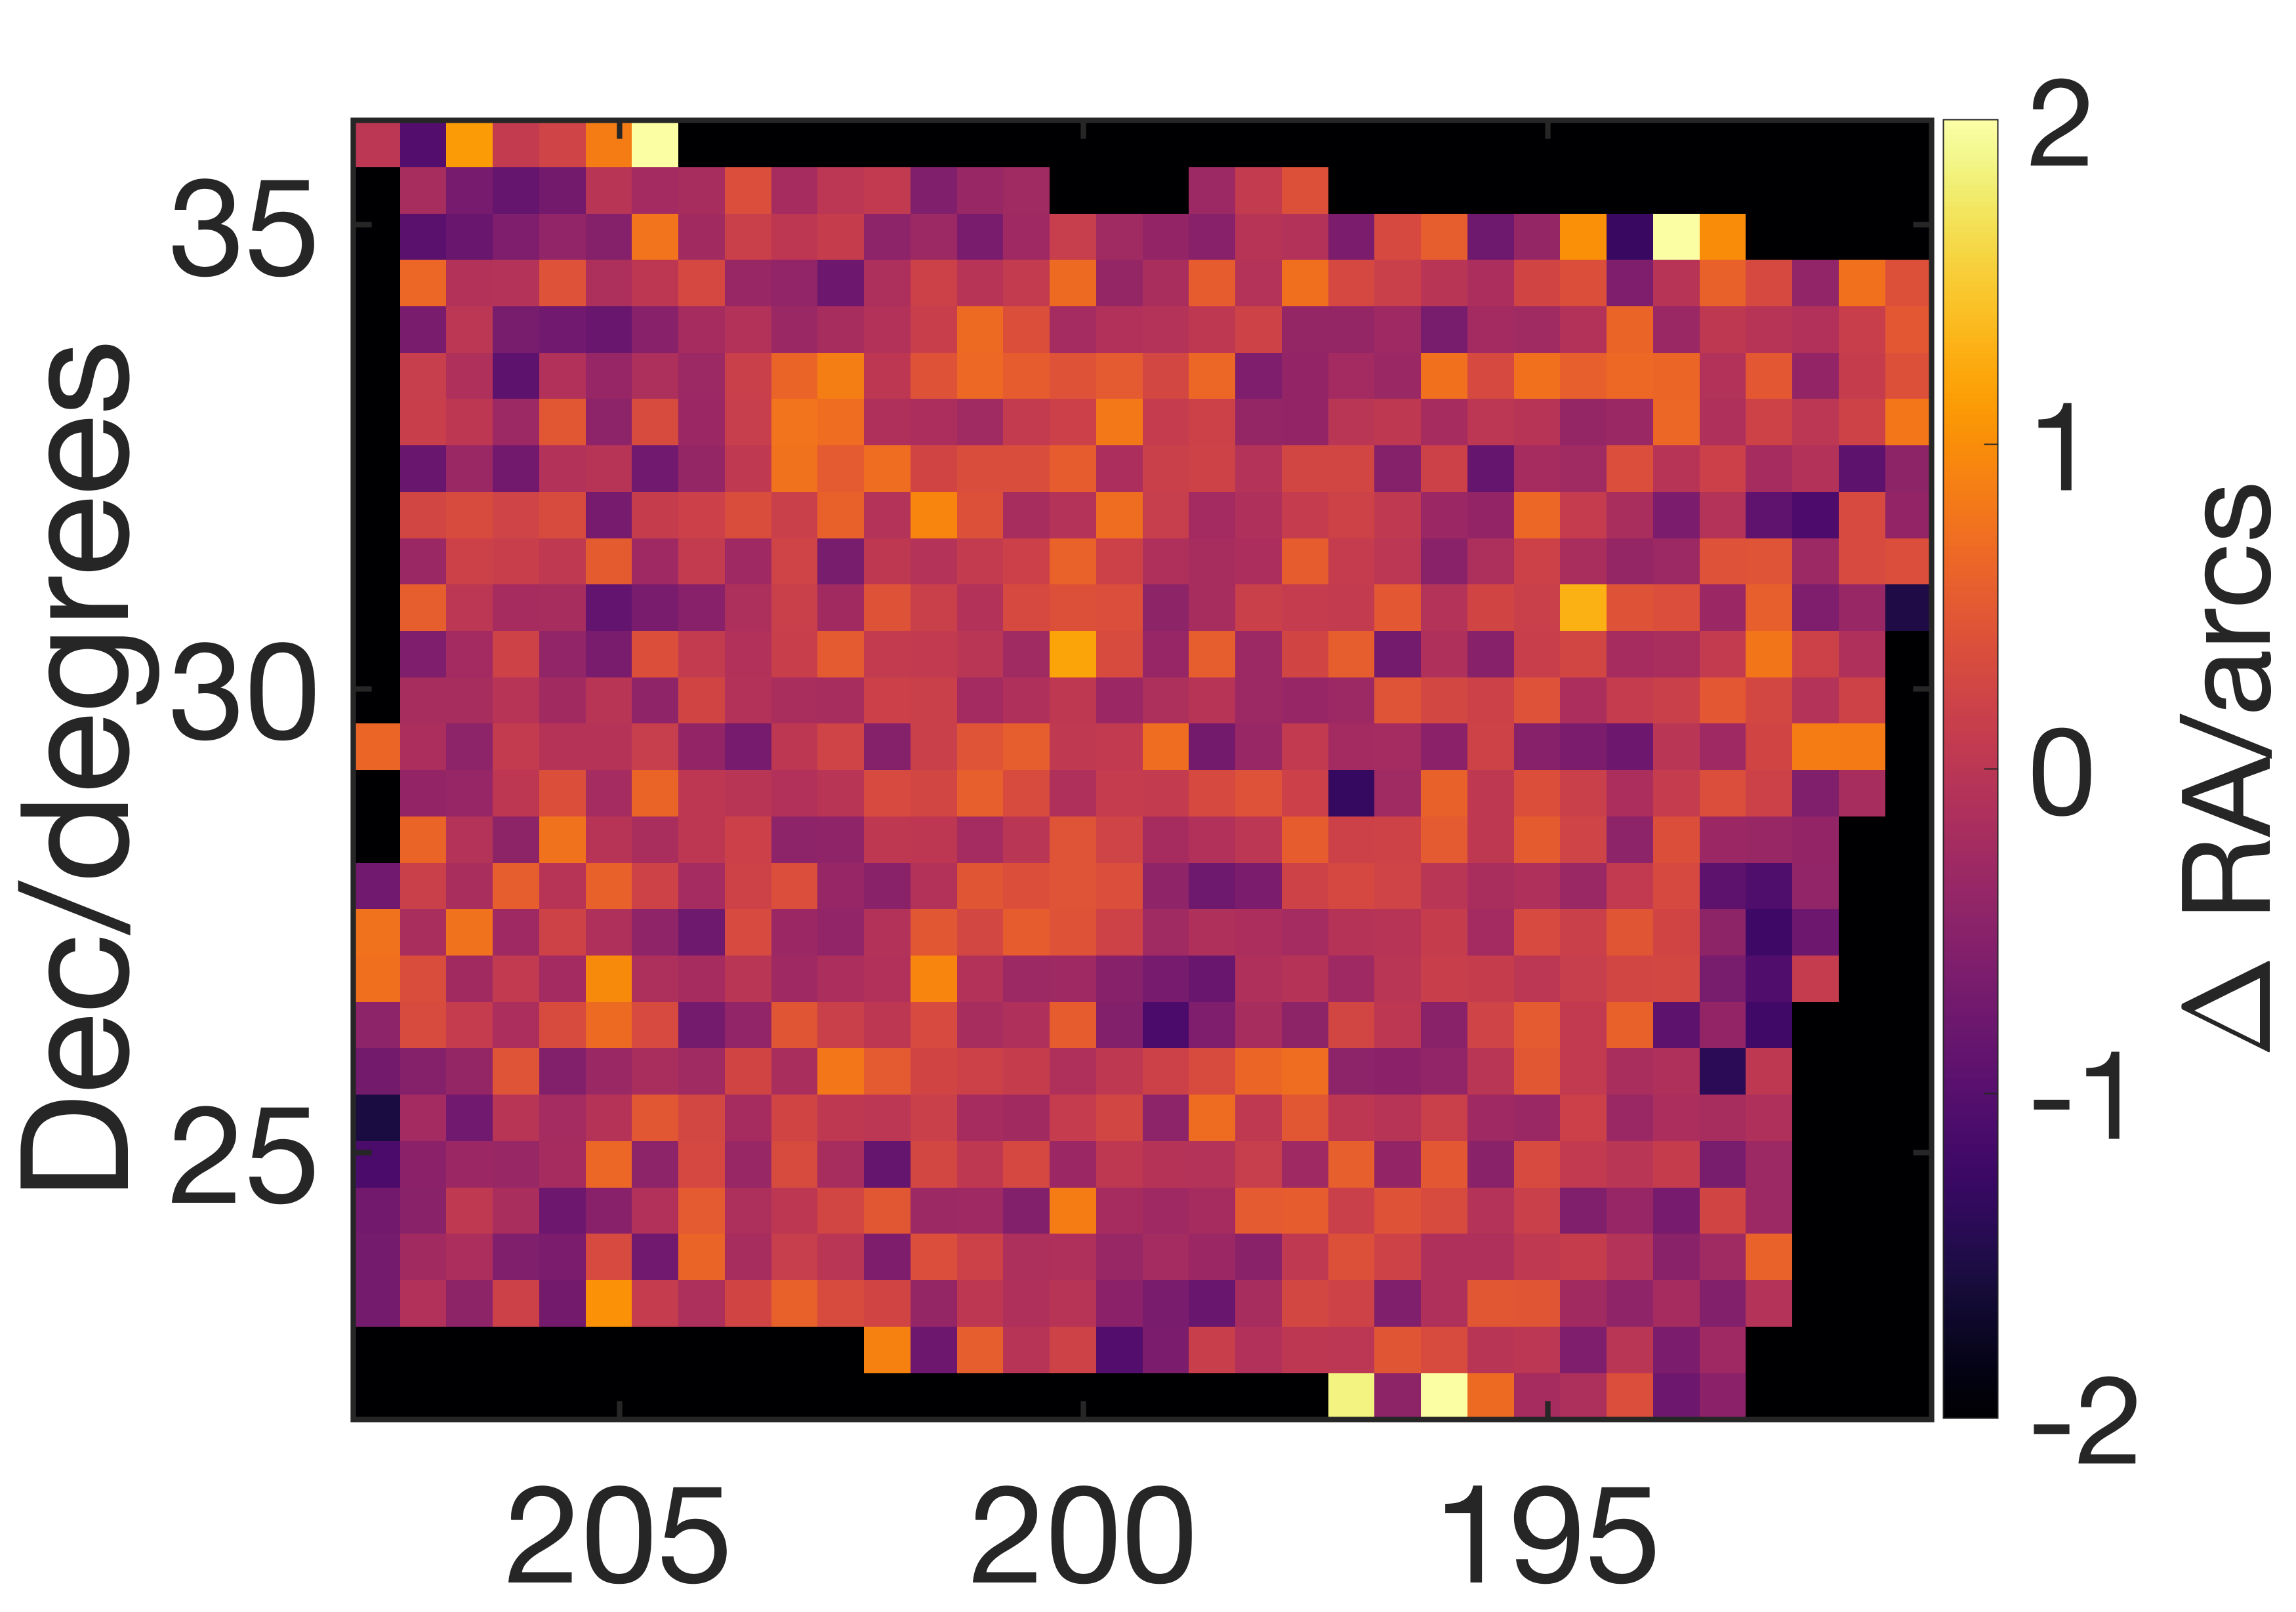
\includegraphics[scale=0.23]{ngp_dra.png} \hspace{5mm}
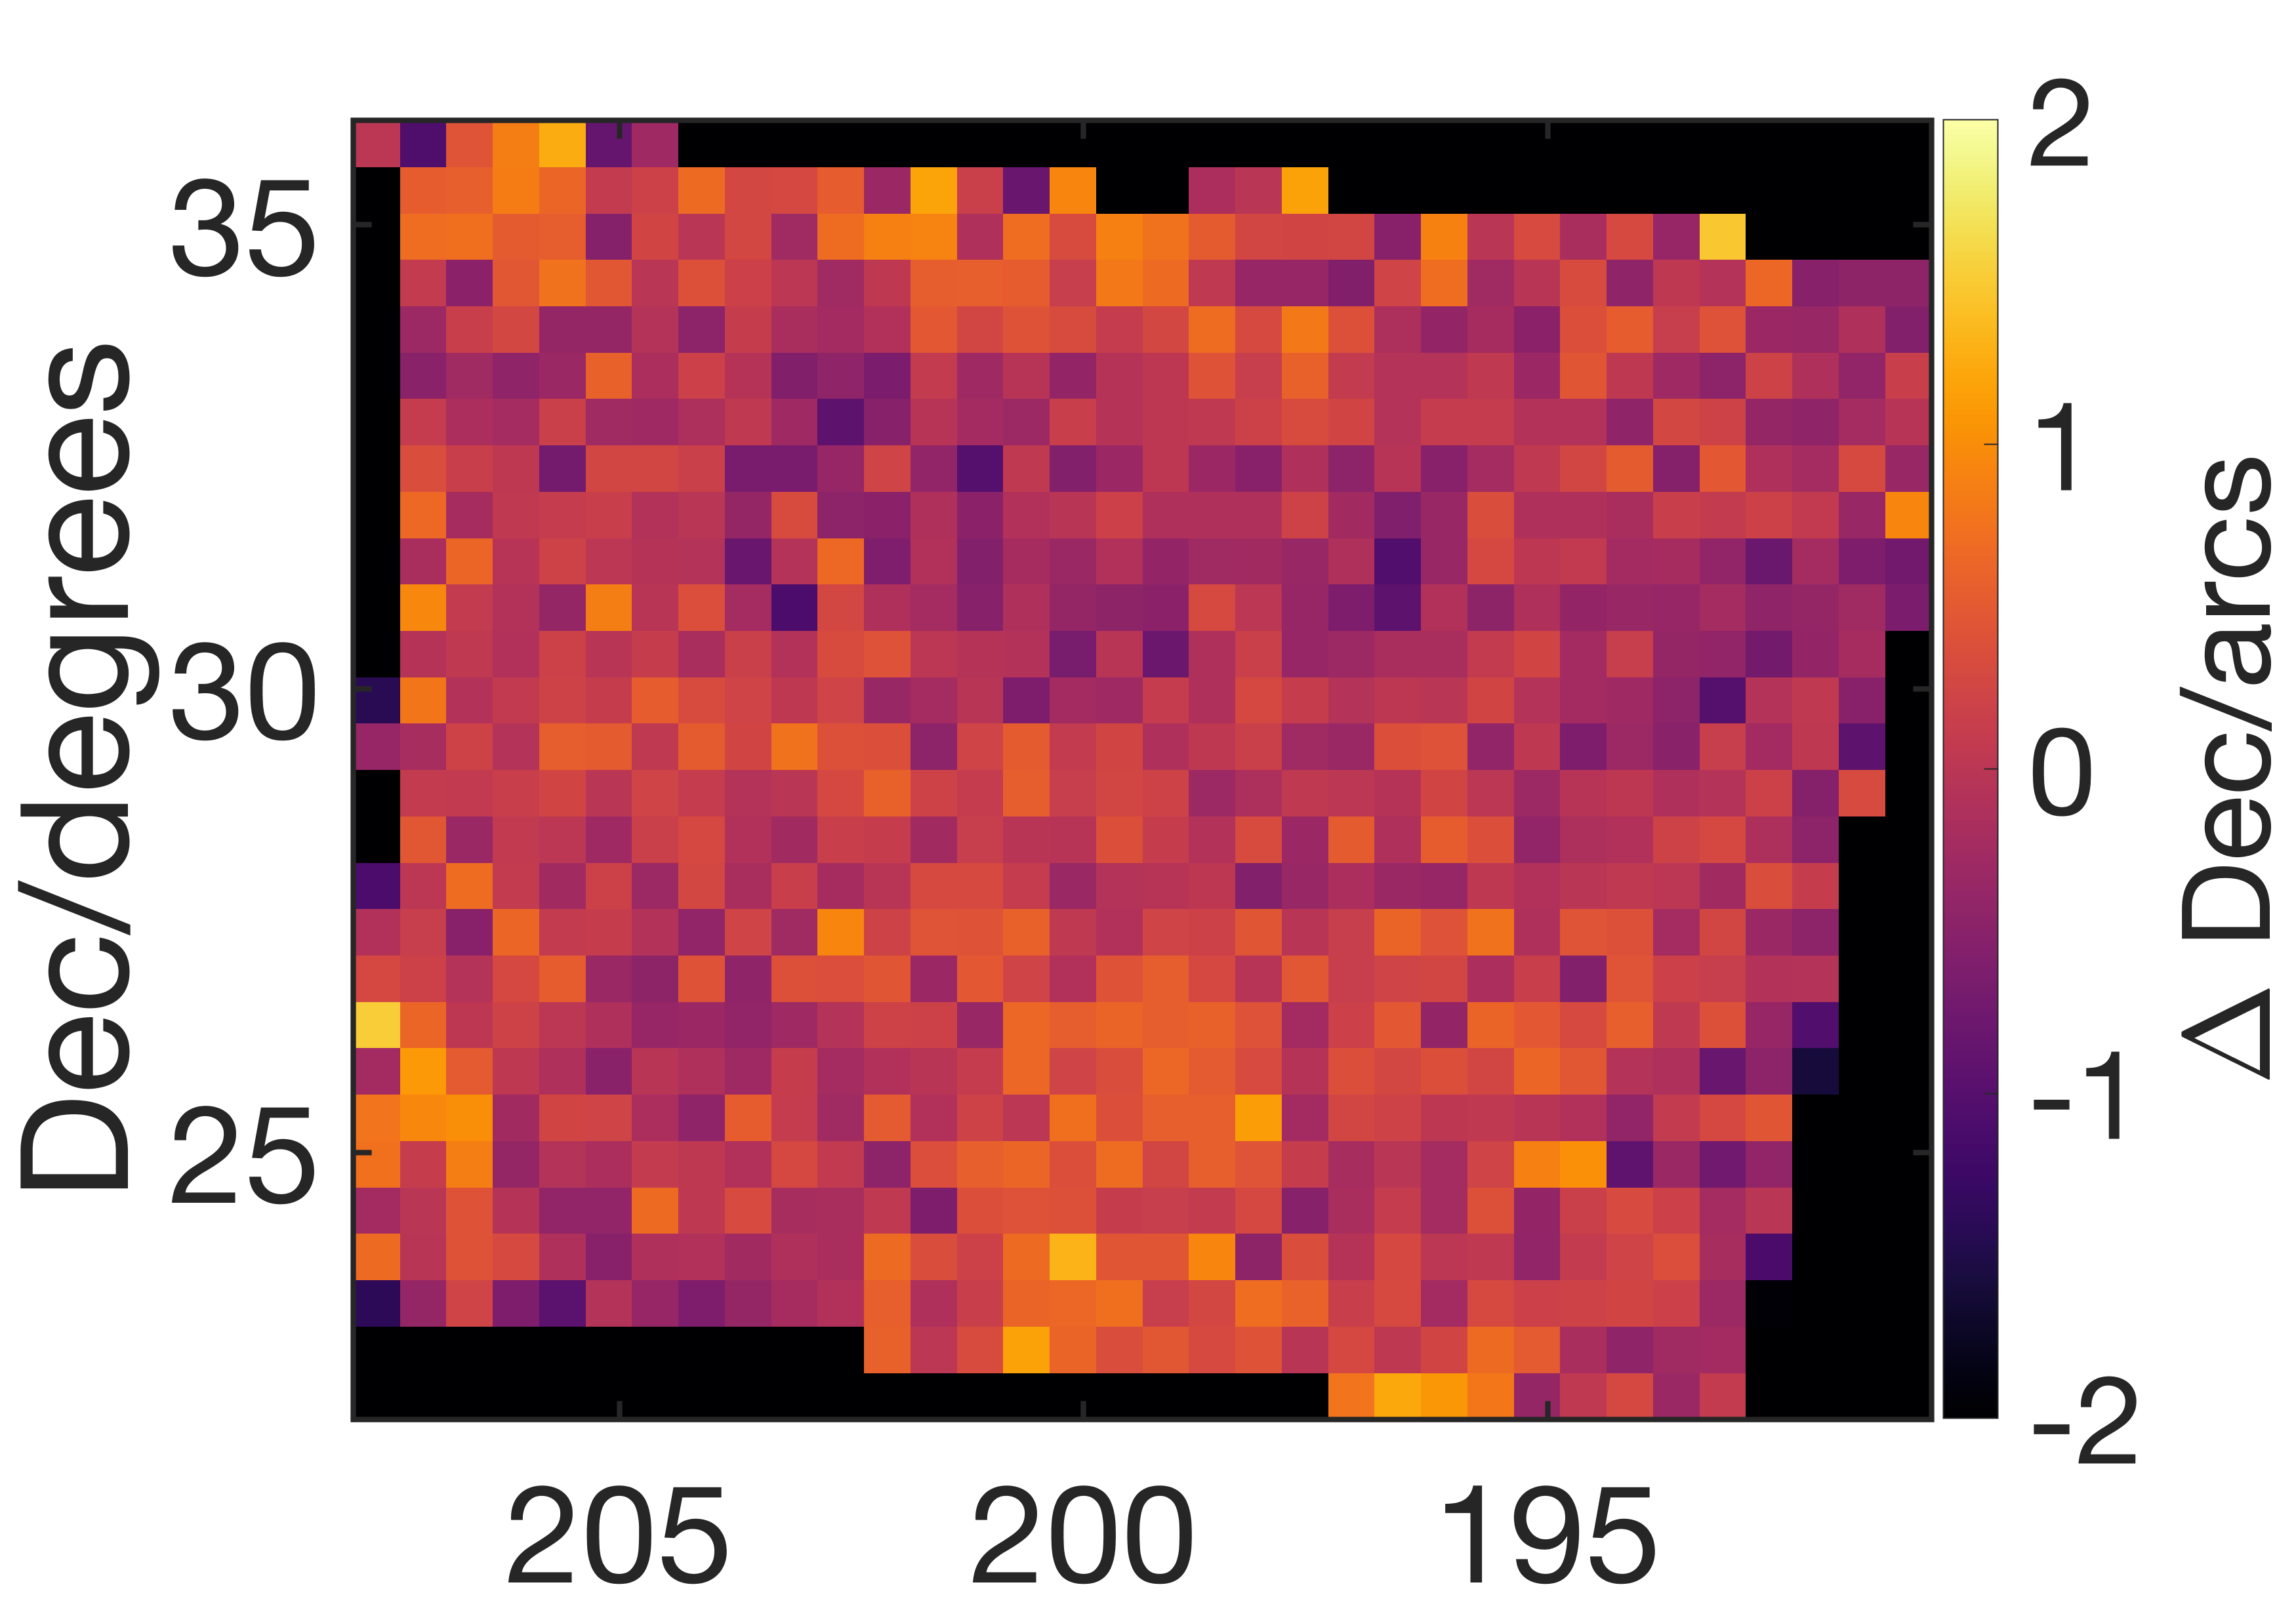
\includegraphics[scale=0.23]{ngp_ddec.png}
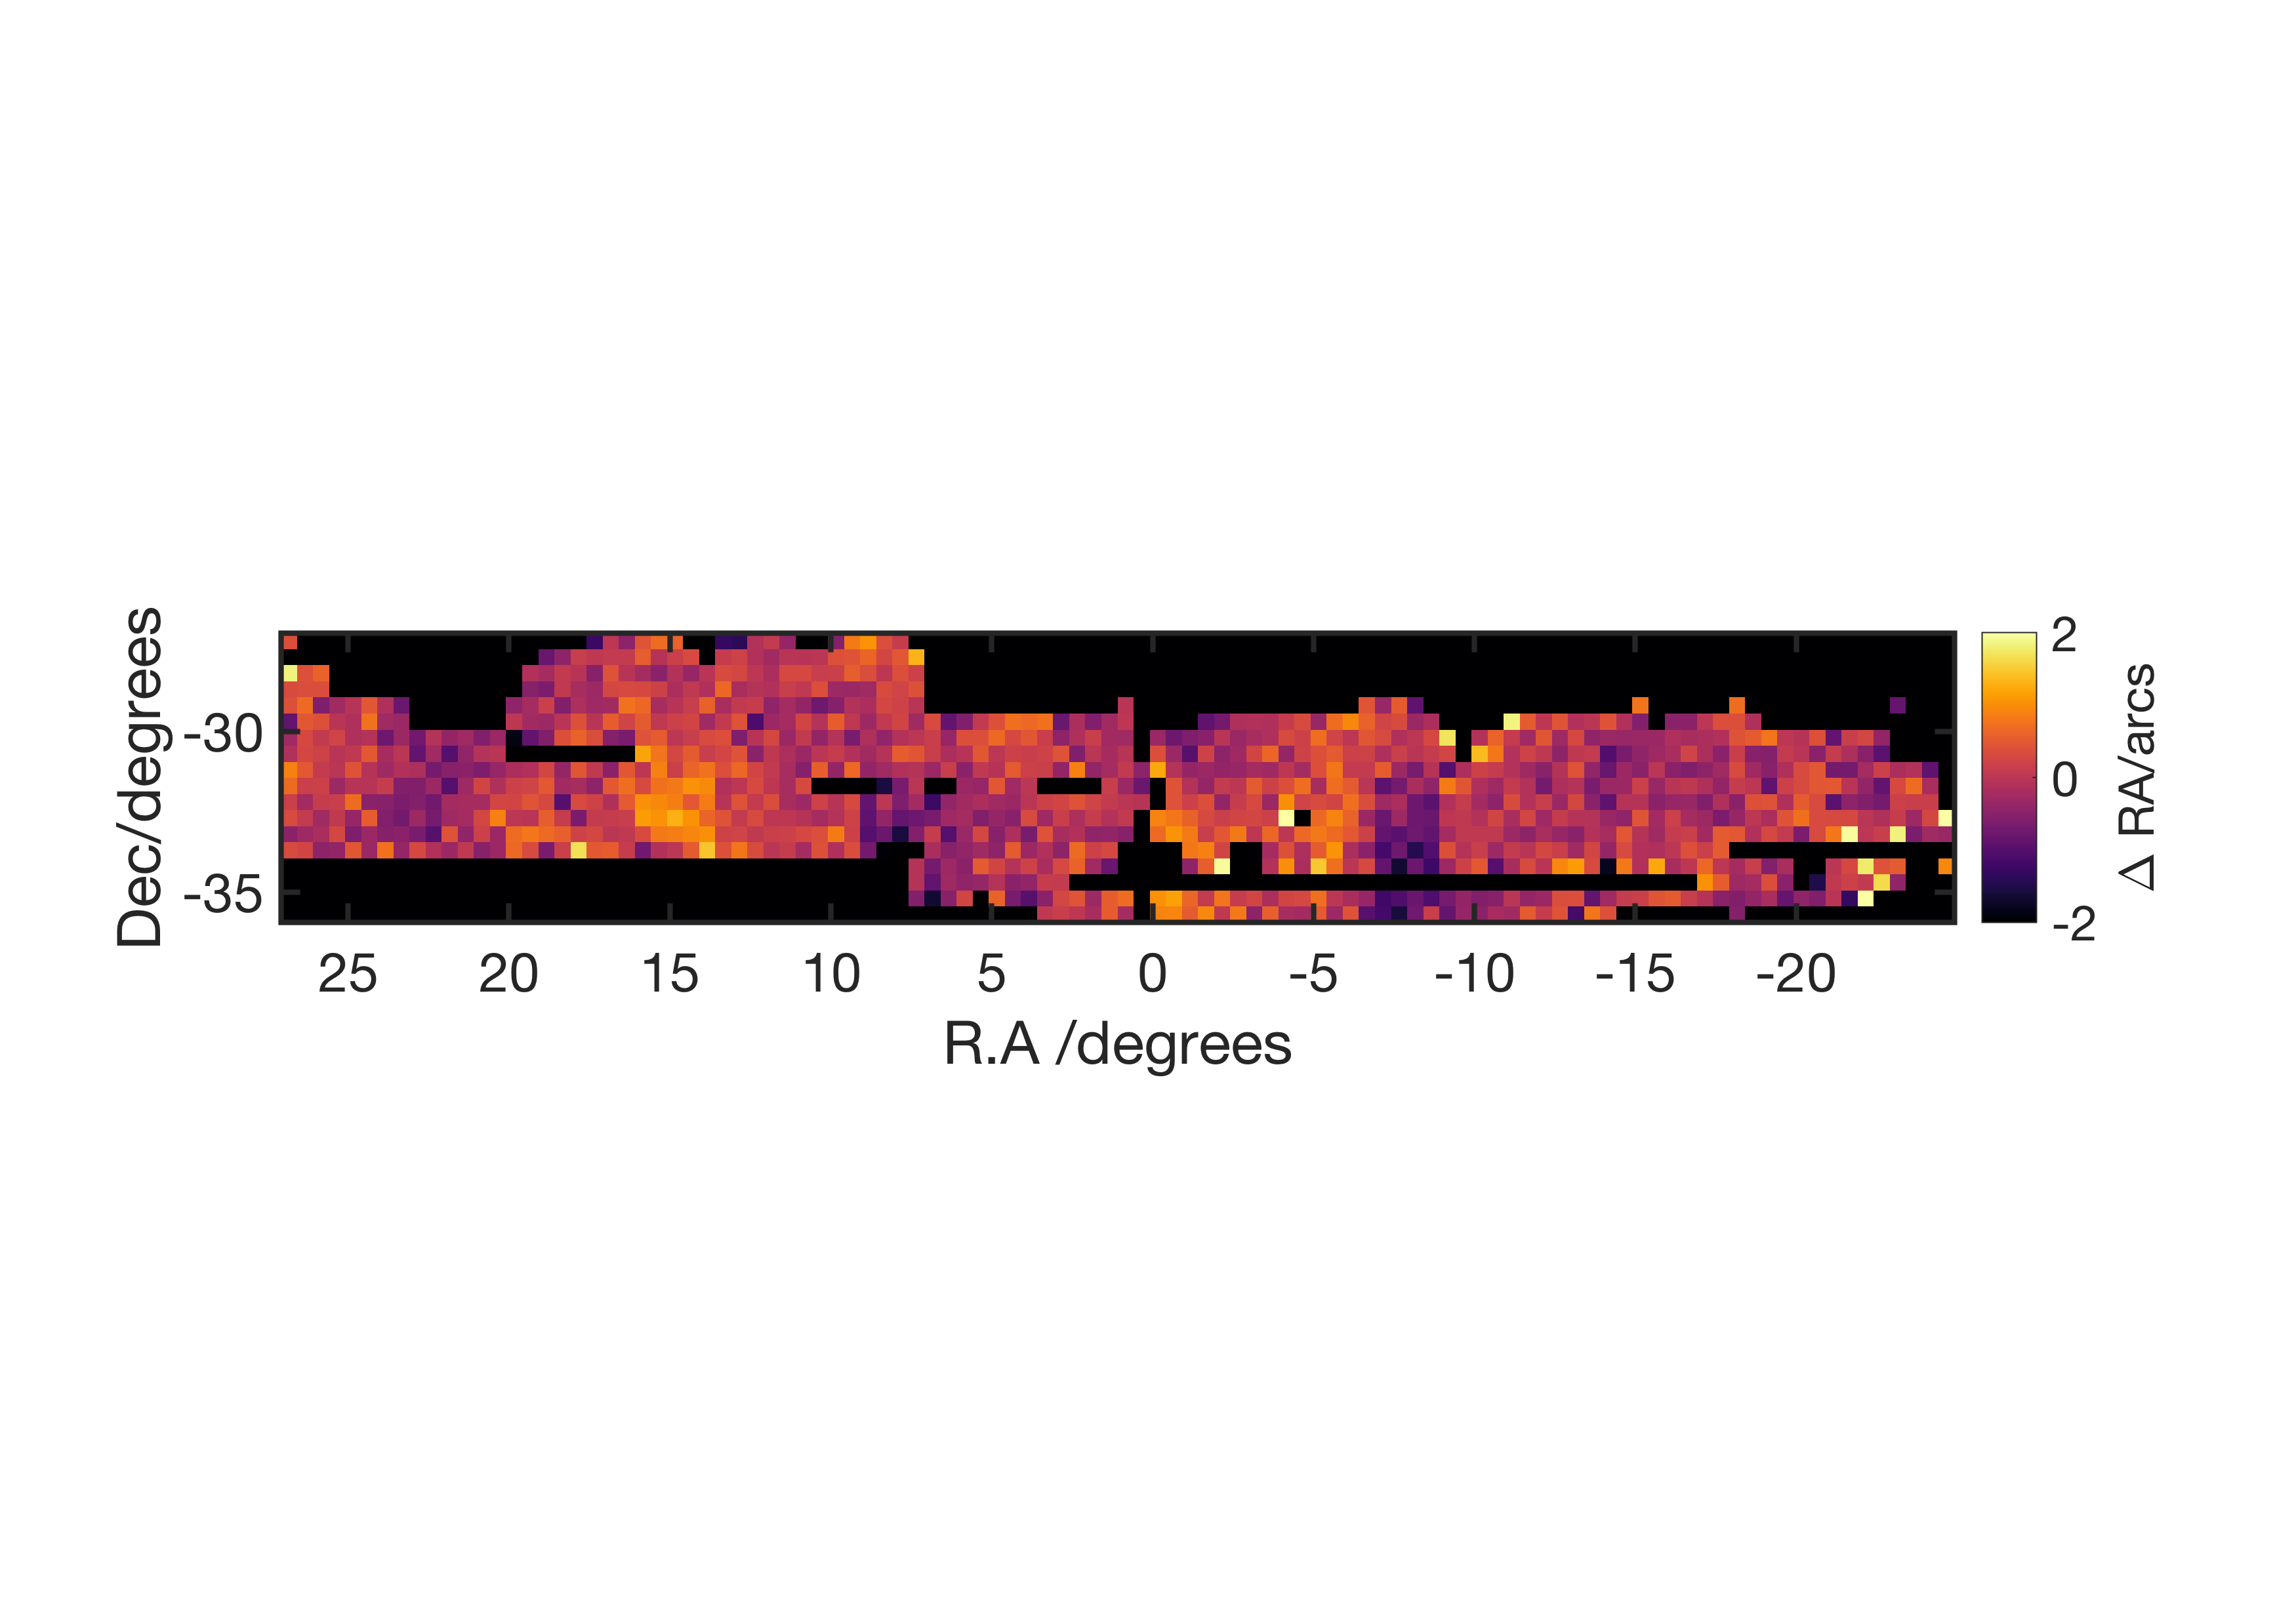
\includegraphics[scale=0.6,trim={0 87mm 0mm 75mm}, clip]{sgp_dra.png}
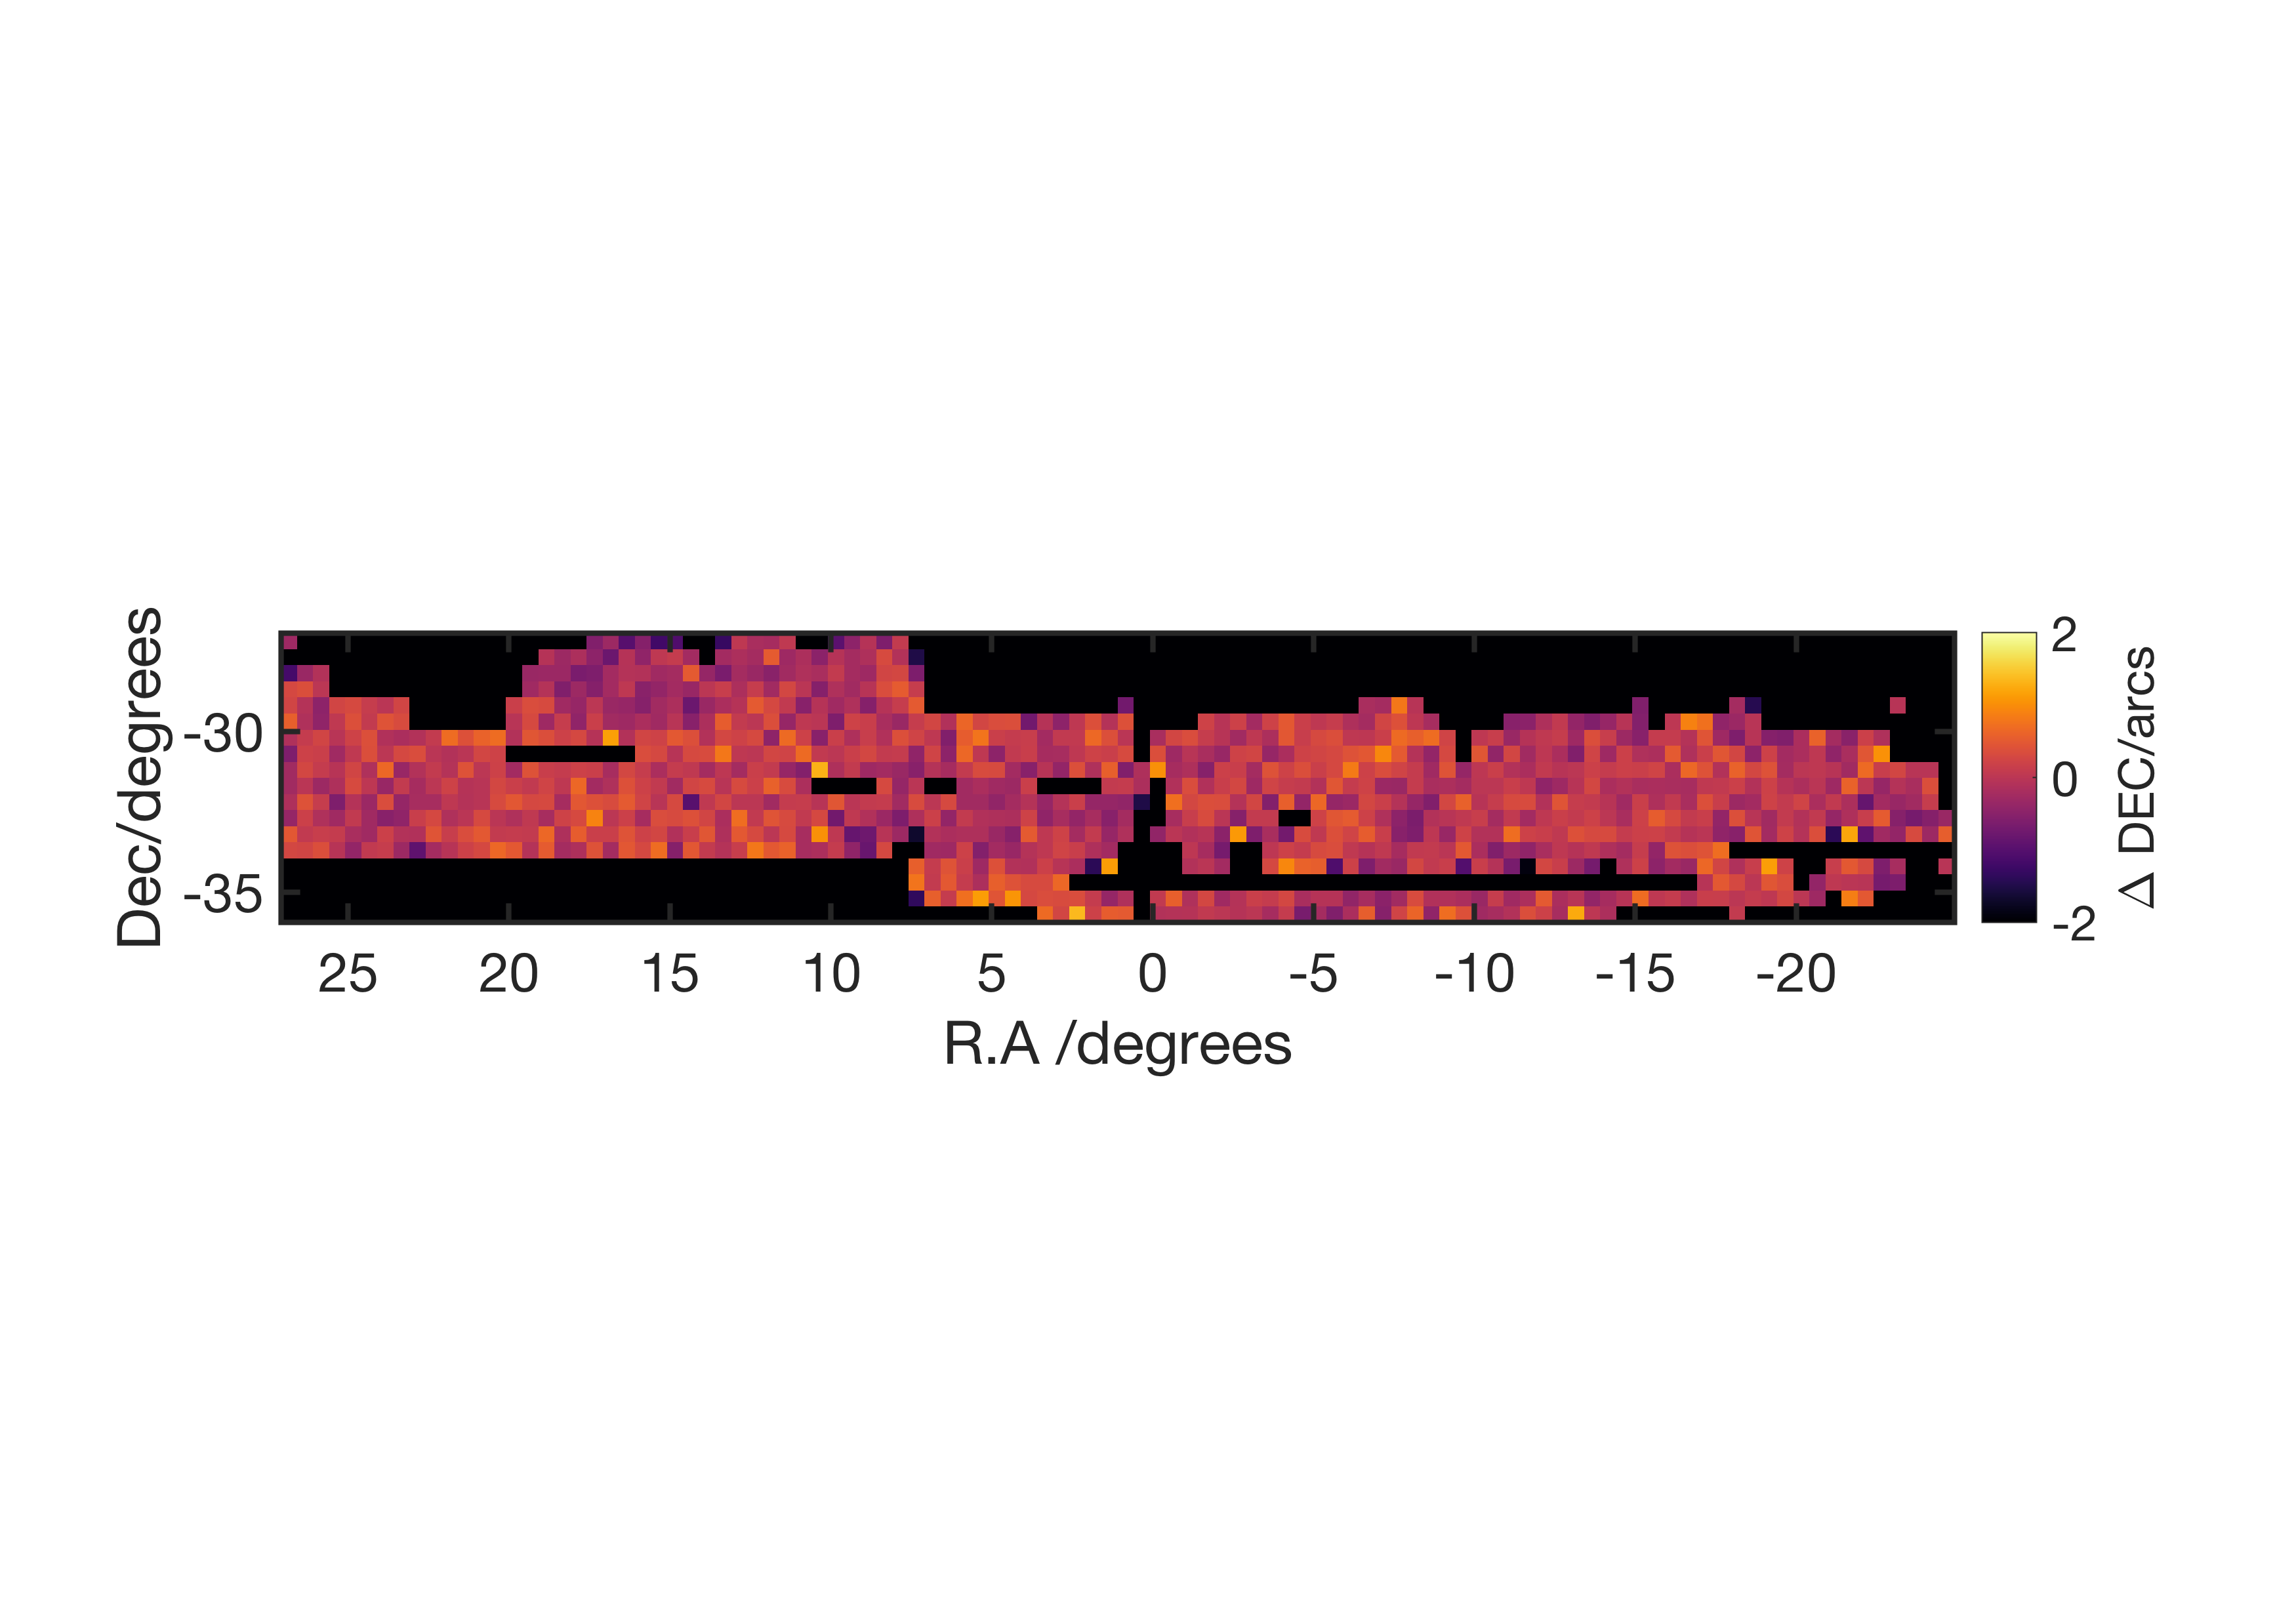
\includegraphics[scale=0.6,trim={0 60mm 0mm 80mm}, clip]{sgp_ddec.png}
\caption{\protect\label{fig_pos_errs} The mean positional errors in
  R.A and Dec. averaged in areas $0.5\times0.5$ deg$^2$ as a
  function of position on the sky for the NGP field and the SGP
  fields. 
}
\end{figure*} 

\subsection{Purity, flux boosting and completeness}

Based on Gaussian statistics, we expect $\simeq$0.2\% of the sources
in the catalogue to be spurious. However, V16 argue that this is
likely to be a significant overestimate because our errors, while being
good estimates of the errors on the flux measurements, are likely to
underestimate 
the signal-to-noise of a detection.

A major problem in submillimetre surveys, where source confusion is usually
an issue, is flux bias or `flux boosting', in which the measured flux densities
are systematically too high. V16 used the in-out simulations to quantify this
effect in the H-ATLAS. Table 6 in V16 gives estimates of the flux bias as
a function of flux density for all three SPIRE bands. The table shows that
at the 4$\sigma$ detection flux density, the measured flux densities are
on average higher than the true flux densities by $\simeq$20\%, 5\% and
4\% at 250 $\mu$m, 350 $\mu$m and 500 $\mu$m, respectively. Astronomers interested
in comparing the flux densities in the catalogue with the predictions of models should be
aware of this effect. Table 6 in V16 can be used to correct the flux densities
for this effect.

V16 also used the in-out simulations to estimate the completeness of the survey as a function
of measured flux density in all three SPIRE bands. This is shown in Figure 21 of V16 and listed in
Table 7 of V16. The completeness at 250 $\mu$m is $\simeq$87\% at the
4$\sigma$ detection limit of the survey.



\section{Summary}

We have described the construction of the source catalogues from
the {\it Herschel} survey of fields 
around the north and south Galactic poles. This survey which was
carried out in five photometric bands - 100, 160, 250, 350 and 500 $\mu$m -
was part of the 
{\it Herschel} Astrophysical Terahertz Large Area Survey
(H-ATLAS), a survey of 660 deg$^2$ 
of the extragalactic sky. Our source catalogues
cover 
285 deg$^2$ around the SGP and 170 deg$^2$
around the NGP.

The catalogues contain
118,986 sources for the NGP field and 183,784 sources for the
SGP field detected at
more than 4$\sigma$ significance in any of the 250\mic, 350\mic or
500\mic bands band. We present photometry in all five bands for
each source, including aperture photometry for sources known to
be extended. We discuss all the practical issues - completeness, reliability,
flux boosting, accuracy of positions, accuracy of flux measurements - necessary to
use the catalogues for astronomical projects.

\section*{Acknowledgments}

PC, LD and SM acknowledge support from the European Research Council (ERC)
in the form of Consolidator Grant {\sc CosmicDust} (ERC-2014-CoG-647939, PI H\,L\,Gomez).
SJM LD and RJI acknowledge
support from the ERC in the form of the Advanced Investi-
gator Program,
COSMICISM
(ERC-2012-ADG
20120216,
PI  R.J.Ivison).
EV and SAE acknowledge funding
from the UK Science and Technology Facilities Council consolidated grant ST/K000926/1.
MS and SAE have received
funding from the European Union Seventh Framework Programme  ([FP7/2007-2013]
[FP7/2007-2011])  under  grant
agreement No. 607254.

\begin{thebibliography}{}

\bibitem[Blain et al.(1993)]{blain93} Blain, A.W. and Longair, M.S. 1993,
MNRAS, 264, 509

\bibitem[Bourne et al.(2016)]{bourne16} Bourne, N. et al. 2016, MNRAS, 462, 1714

\bibitem[Chapin et al.(2011)]{chap2011} Chapin, E.L. et al. 2011, MNRAS, 411, 505

\bibitem[Dunne et al.(2011)]{dunne2011} Dunne, L. et al. 2011, MNRAS, 417, 1510

\bibitem[Eales et al.(2010)]{eales2010} Eales, S., et al.\ 2010,  \pasp, 122, 499 

\bibitem[Eales et al.(2017)]{eales2017} Eales, S., et al.\ 2017, MNRAS, in press
(arXiv: 1710.01314)

\bibitem[Fudamoto  et al.(2017)]{fud2017} Fudamoto, Y. et al. 2017,
MNRAS, 472, 2028

\bibitem[Furlanetto et al.(2017)]{furl2017} Furlanetto, C. et al. 2017,
MNRAS, submitted (F17; Paper III)

\bibitem[Griffin et al. (2010)]{spire} Griffin, M.J. et al. 2010 A\&A, 518, L3

\bibitem[Griffin et al. (2013)]{griffin2013} Griffin, M.J. et al. 2013,
MNRAS, 434, 992

\bibitem[Ibar et al. (2010)]{pacsmaps} Ibar, E., 2010, MNRAS, 409, 38

\bibitem[Neugebauer et al. (1984)]{neugebauer84} Neugebauer, G. et al. 1984,
ApJ, 278, L1

\bibitem[Pascale et al. (2011)]{spiremaps} Pascale, E., et al. 2011, MNRAS, 415, 911 

\bibitem[Pearson et al. (2013)]{pearson2003} Pearson, E.A. et al. 2013, MNRAS, 435,
2753

\bibitem[\protect\citeauthoryear{{Pilbratt}}{{Pilbratt et al.}}{2010}]{herschel} Pilbratt, G.~L., et al. A\&A, 518, L1

\bibitem[Poglitsch et al. (2010)]{pacs} Poglitsch, A., et al. 2010 A\&A, 518, L2

\bibitem[Rigby et al. (2011)]{rigby2011} Rigby, E.E, et al. 2011, MNRAS, 415, 2336 

\bibitem[Shanks et al. (2015)]{shanks15} Shanks, T. et al. 2015, MNRAS, 451, 4238

\bibitem[Smith et al. (2011)]{Smith11} Smith, D.J.B. et al. 2011, MNRAS, 
416, 857

\bibitem[Smith et al. (2017)]{Smith17} Smith, M.W.L. et al. 2017, ApJ suppl., in press
(S17; Paper I)

\bibitem[Valiante et al. (2016)]{val2016} Valiante, E. et al. 2016, MNRAS, 462, 3146
(V16)

\bibitem[Zavala et al. (2017)]{zav2017} Zavala, J.A. et al. 2017, Nature Astronomy,
in press (arXiv: 1707.09022)

\end{thebibliography}
\label{lastpage}

\end{document}

